% =================================================
% 性学系列 · 亲密实践与技巧
% 共享基座见 common.tex
% =================================================
\documentclass[12pt,UTF8,openany]{ctexbook}
% =================================================
% common.tex —— 性学系列 共享基座
% 导言区 / 配色 / TikZ 库 / ctexset / C 列型 / 字体 / 书眉页码
% 各册 % =================================================
% common.tex —— 性学系列 共享基座
% 导言区 / 配色 / TikZ 库 / ctexset / C 列型 / 字体 / 书眉页码
% 各册 % =================================================
% common.tex —— 性学系列 共享基座
% 导言区 / 配色 / TikZ 库 / ctexset / C 列型 / 字体 / 书眉页码
% 各册 \input{common.tex} 引用
% =================================================
\usepackage[top=2.5cm,bottom=2.5cm,left=2.6cm,right=2.6cm,headheight=2.0cm]{geometry}
\usepackage{amsmath}
\usepackage{amssymb}
\usepackage{array}
\usepackage{tabularx}
\usepackage{multirow}
\usepackage{booktabs}
\usepackage{enumitem}
\usepackage{xcolor}
\usepackage{graphicx}
\usepackage{tikz}
\usetikzlibrary{positioning,calc,arrows.meta,shapes.geometric,matrix}
\definecolor{myblue}{HTML}{185FA5}
\definecolor{myblueL}{HTML}{E6F1FB}
\definecolor{mygreen}{HTML}{3B6D11}
\definecolor{mygreenL}{HTML}{C0DD97}
\definecolor{myteal}{HTML}{1D9E75}
\definecolor{myamber}{HTML}{854F0B}
\definecolor{myamberL}{HTML}{FAEEDA}
\definecolor{myred}{HTML}{A32D2D}
\definecolor{myredL}{HTML}{FCEBEB}
\definecolor{mypurple}{HTML}{534AB7}
\definecolor{mypurpleL}{HTML}{EEEDFE}
\definecolor{mycoral}{HTML}{D85A30}
\definecolor{mycoralL}{HTML}{FAECE7}
\definecolor{mypink}{HTML}{D4537E}
\definecolor{mypinkL}{HTML}{F4C0D1}
\definecolor{mypinkM}{HTML}{ED93B1}
\definecolor{mygray}{HTML}{888780}

% 字体
\setCJKfamilyfont{hei}{SimHei}
\newcommand{\myhei}{\CJKfamily{hei}}

% 书眉与页码（印刷友好：中文页眉 + 居中页码）
\usepackage{fancyhdr}
\pagestyle{fancy}
\fancyhf{}
\fancyhead[L]{\small\myhei 性学系列}
\fancyhead[R]{\small\leftmark}
\fancyfoot[C]{\small\thepage}
\renewcommand{\headrulewidth}{0.4pt}
\fancypagestyle{plain}{\fancyhf{}\fancyfoot[C]{\small\thepage}\renewcommand{\headrulewidth}{0pt}}
\fancypagestyle{empty}{\fancyhf{}\renewcommand{\headrulewidth}{0pt}}

% 行距（零基础易读，略松）
\linespread{1.3}

% 超链接：印刷友好（黑色，电子版仍可点击）
\usepackage[colorlinks,linkcolor=black,citecolor=black,urlcolor=black]{hyperref}

\ctexset{
  chapter/name={第,章},
  chapter/number={\arabic{chapter}},
  section/format=\Large\bfseries,
}

\newcolumntype{C}{>{\centering\arraybackslash}X}
 引用
% =================================================
\usepackage[top=2.5cm,bottom=2.5cm,left=2.6cm,right=2.6cm,headheight=2.0cm]{geometry}
\usepackage{amsmath}
\usepackage{amssymb}
\usepackage{array}
\usepackage{tabularx}
\usepackage{multirow}
\usepackage{booktabs}
\usepackage{enumitem}
\usepackage{xcolor}
\usepackage{graphicx}
\usepackage{tikz}
\usetikzlibrary{positioning,calc,arrows.meta,shapes.geometric,matrix}
\definecolor{myblue}{HTML}{185FA5}
\definecolor{myblueL}{HTML}{E6F1FB}
\definecolor{mygreen}{HTML}{3B6D11}
\definecolor{mygreenL}{HTML}{C0DD97}
\definecolor{myteal}{HTML}{1D9E75}
\definecolor{myamber}{HTML}{854F0B}
\definecolor{myamberL}{HTML}{FAEEDA}
\definecolor{myred}{HTML}{A32D2D}
\definecolor{myredL}{HTML}{FCEBEB}
\definecolor{mypurple}{HTML}{534AB7}
\definecolor{mypurpleL}{HTML}{EEEDFE}
\definecolor{mycoral}{HTML}{D85A30}
\definecolor{mycoralL}{HTML}{FAECE7}
\definecolor{mypink}{HTML}{D4537E}
\definecolor{mypinkL}{HTML}{F4C0D1}
\definecolor{mypinkM}{HTML}{ED93B1}
\definecolor{mygray}{HTML}{888780}

% 字体
\setCJKfamilyfont{hei}{SimHei}
\newcommand{\myhei}{\CJKfamily{hei}}

% 书眉与页码（印刷友好：中文页眉 + 居中页码）
\usepackage{fancyhdr}
\pagestyle{fancy}
\fancyhf{}
\fancyhead[L]{\small\myhei 性学系列}
\fancyhead[R]{\small\leftmark}
\fancyfoot[C]{\small\thepage}
\renewcommand{\headrulewidth}{0.4pt}
\fancypagestyle{plain}{\fancyhf{}\fancyfoot[C]{\small\thepage}\renewcommand{\headrulewidth}{0pt}}
\fancypagestyle{empty}{\fancyhf{}\renewcommand{\headrulewidth}{0pt}}

% 行距（零基础易读，略松）
\linespread{1.3}

% 超链接：印刷友好（黑色，电子版仍可点击）
\usepackage[colorlinks,linkcolor=black,citecolor=black,urlcolor=black]{hyperref}

\ctexset{
  chapter/name={第,章},
  chapter/number={\arabic{chapter}},
  section/format=\Large\bfseries,
}

\newcolumntype{C}{>{\centering\arraybackslash}X}
 引用
% =================================================
\usepackage[top=2.5cm,bottom=2.5cm,left=2.6cm,right=2.6cm,headheight=2.0cm]{geometry}
\usepackage{amsmath}
\usepackage{amssymb}
\usepackage{array}
\usepackage{tabularx}
\usepackage{multirow}
\usepackage{booktabs}
\usepackage{enumitem}
\usepackage{xcolor}
\usepackage{graphicx}
\usepackage{tikz}
\usetikzlibrary{positioning,calc,arrows.meta,shapes.geometric,matrix}
\definecolor{myblue}{HTML}{185FA5}
\definecolor{myblueL}{HTML}{E6F1FB}
\definecolor{mygreen}{HTML}{3B6D11}
\definecolor{mygreenL}{HTML}{C0DD97}
\definecolor{myteal}{HTML}{1D9E75}
\definecolor{myamber}{HTML}{854F0B}
\definecolor{myamberL}{HTML}{FAEEDA}
\definecolor{myred}{HTML}{A32D2D}
\definecolor{myredL}{HTML}{FCEBEB}
\definecolor{mypurple}{HTML}{534AB7}
\definecolor{mypurpleL}{HTML}{EEEDFE}
\definecolor{mycoral}{HTML}{D85A30}
\definecolor{mycoralL}{HTML}{FAECE7}
\definecolor{mypink}{HTML}{D4537E}
\definecolor{mypinkL}{HTML}{F4C0D1}
\definecolor{mypinkM}{HTML}{ED93B1}
\definecolor{mygray}{HTML}{888780}

% 字体
\setCJKfamilyfont{hei}{SimHei}
\newcommand{\myhei}{\CJKfamily{hei}}

% 书眉与页码（印刷友好：中文页眉 + 居中页码）
\usepackage{fancyhdr}
\pagestyle{fancy}
\fancyhf{}
\fancyhead[L]{\small\myhei 性学系列}
\fancyhead[R]{\small\leftmark}
\fancyfoot[C]{\small\thepage}
\renewcommand{\headrulewidth}{0.4pt}
\fancypagestyle{plain}{\fancyhf{}\fancyfoot[C]{\small\thepage}\renewcommand{\headrulewidth}{0pt}}
\fancypagestyle{empty}{\fancyhf{}\renewcommand{\headrulewidth}{0pt}}

% 行距（零基础易读，略松）
\linespread{1.3}

% 超链接：印刷友好（黑色，电子版仍可点击）
\usepackage[colorlinks,linkcolor=black,citecolor=black,urlcolor=black]{hyperref}

\ctexset{
  chapter/name={第,章},
  chapter/number={\arabic{chapter}},
  section/format=\Large\bfseries,
}

\newcolumntype{C}{>{\centering\arraybackslash}X}


\begin{document}

% ===== 封面 =====
\begin{titlepage}
\centering
\vspace*{1.5cm}
\begin{tikzpicture}
\draw[myblue,line width=2pt] (0,0) circle (1.2);
\node[text=white] at (0,0) {\myhei\zihao{3}性};
\end{tikzpicture}
\vspace{0.6cm}
\noindent\rule{\textwidth}{0.4pt}
\vspace{0.5cm}
\myhei\zihao{5} 性学系列\,·\,家庭健康科普\,·\,全五册
\vspace{2.5cm}
\myhei\zihao{0} 亲密实践与技巧\par
\vspace{1.2cm}
\itshape\zihao{3} 从「会做」到「做得更好」\par
\vspace{5.2cm}
\noindent\rule{\textwidth}{0.4pt}
\vspace{0.5cm}
\zihao{5} 性学系列\,·\,\today
\end{titlepage}

% ===== 免责声明 =====
\begin{center}\zihao{5}\itshape
本书为家庭健康科普读物，内容力求科学严谨，但\textbf{不替代专业医生的诊断与治疗}。\\
涉及个人健康问题，请以正规医疗机构的检查与建议为准。\\
全书以安全、自愿、相互尊重为底色，尊重多元与个体差异。\par\end{center}
\clearpage

% ===== 如何使用本书 =====
\chapter*{如何使用本书}
\addcontentsline{toc}{chapter}{如何使用本书}
\noindent\textbf{性学系列共五册：}
\begin{itemize}[leftmargin=2em]
\item \textbf{A 性健康基础} —— 认知、同意、防护、STI、避孕总论（建议先读）
\item \textbf{B 亲密实践与技巧} —— 前戏、体位、高潮引导、呼吸与盆底
\item \textbf{C 男性性健康} —— 男性解剖、ED/自慰、绝育、不育
\item \textbf{D 女性性健康} —— 女性解剖、妇科、不孕、人流、避孕、孕期/更年期
\item \textbf{E BDSM 与 Kink} —— 安全框架下的亲密表达
\end{itemize}
\vspace{0.6em}
\noindent\textbf{建议阅读路径（零基础）：} 先通读 A 建立认知与安全底线 → 按需读 C 或 D 了解自己的身体 → 再读 B 学技巧 → 兴趣到了再读 E。每章末有“一页要点”可快读。
\clearpage

% ===== 目录 =====
\tableofcontents
\clearpage
\chapter{见面了怎么办：从邀约到在场的清单}
\label{chap:meeting}

"见面"这件事，焦虑往往来自不确定。把流程拆开，每一步都知道该做什么，就不慌了。
本章按时间顺序分为三个阶段，并给出各自的红线。

\section{见面前：先把安全底线定好}

\begin{itemize}[leftmargin=2em]
  \item \textbf{选对场合}：第一次见面选\textbf{公共场所}（咖啡馆、商场、公园），
        时间尽量在白天或傍晚，不去对方指定的私密场所或陌生地点。
  \item \textbf{自己来、自己走}：自己安排交通，不搭对方的车去偏僻处；
        告知朋友或家人去哪、和谁、大概几点回。
  \item \textbf{管好饮品}：饮料或杯子不离视线；离开过又回来的不再喝；不接受陌生人递来的酒。
  \item \textbf{提前想清楚边界}：去之前就问自己——能接受到哪一步？什么情况一定喊停？
        把答案在心里定好，现场就不容易被带着走。
  \item \textbf{信任直觉}：如果对方催你换地方、要求保密、或不尊重你说"不"，这些都是信号。
\end{itemize}

\section{见面中：感受与沟通}

\begin{itemize}[leftmargin=2em]
  \item \textbf{先感受自己}：放松吗？还是隐隐不安？身体紧绷、想离开的念头，
        都是重要信号，别忽略。
  \item \textbf{边界说在前面}：在气氛还好时自然地说"我今天想先聊聊天""我不去太晚的地方"。
        提前说比临场拒绝容易得多。
  \item \textbf{随时可以停}：任何时刻不舒服，直接说"我想回去了"即可，不必解释到对方满意。
  \item \textbf{观察对方对你说"不"的反应}：提一个小要求或小拒绝，看他是尊重还是施压、冷脸、纠缠——
        这能看出这个人值不值得继续。
  \item \textbf{别被酒精带节奏}：微醺会降低判断力，保持清醒才能真正地同意或拒绝。
\end{itemize}

\section{想继续亲密：现场的四个确认}

\begin{enumerate}[leftmargin=2em,itemsep=0.3em]
  \item \textbf{确认同意}：双方都清醒、自愿、能随时喊停。"不抗拒"不等于"同意"，
        需要明确的肯定。
  \item \textbf{安全套（避孕套）准备好}：自己备好、在有效期内、知道怎么用，别指望对方一定有。
  \item \textbf{谈避孕与检测}：可以自然地说"我们用安全套好吗""你最近做过检测吗"——
        这不是扫兴，是负责。
  \item \textbf{慢一点、多沟通}：节奏由双方舒服的程度决定；疼、不适、犹豫就停。
        第一次不理想很正常，不必有压力。
\end{enumerate}

\noindent\textbf{三条红线（碰到就走）}：无保护也无所谓、对方不情愿还硬来、
用感情或压力逼你改变决定。任何一条出现，立刻停止、离开、联系朋友。

\section{见面之后}

\begin{itemize}[leftmargin=2em]
  \item \textbf{沟通感受}：事后可简单聊聊彼此的感受，好的和不好的都可以说。
  \item \textbf{留意身体}：如有无保护行为，记住时间窗——紧急避孕越早越好，
        HIV 暴露后预防（PEP）72 小时内；需要时按第~\ref{chap:sti}~章安排检测。
  \item \textbf{保护隐私}：若对方拍摄私密影像，未经你同意不得传播；
        遇到胁迫，第一时间求助（110 / 12320 / 可信任的人）。
  \item \textbf{允许自己复盘}：不管结果如何，想想"哪些我做对了、哪些下次可以不同"，这就是成长。
\end{itemize}

\noindent\textbf{一句话总结}：见面的核心不是"表现好"，而是\textbf{安全 + 自愿 + 能随时喊停}。
守住这三点，其余的慢慢来就好。

\chapter{到了私密场所后：以酒店为例的具体清单}
\label{chap:private}

进了房间\textbf{不等于同意任何事}。环境变了，权利一点没变——同意依然必须清醒、
自愿、可随时撤回。而且这种场景封闭、隐蔽、退路少，反而更要主动把安全底线再确认一遍。
下面按时间顺序拆成四步：进房间 $\to$ 定边界 $\to$ 过程中 $\to$ 之后。

\section{第一步：进房间，先花两分钟看环境}

\begin{itemize}[leftmargin=2em]
  \item 选正规、口碑好的酒店，\textbf{自己登记、自己开门}；进门先试门锁能否正常反锁、
        防盗扣是否完好。
  \item 给朋友或家人发个房号/定位；\textbf{手机充满电}，放在伸手可及的地方。
  \item 别急着放松，先做一次快速隐私排查（见下）。
\end{itemize}

\subsection*{关于偷拍：先纠正一个流传很广的误区}

网上说"关灯用手机摄像头扫，有红点就是针孔摄像头"——\textbf{这个方法基本不靠谱}。
科技日报、中国新闻网均指出：绝大多数针孔摄像头因体积限制没有夜视红外功能，不会发红光；
而现在的手机镜头大多带滤光片，即便有红外光也显示不出来。

更实用的笨办法：

\begin{enumerate}[leftmargin=2em,itemsep=0.3em]
  \item \textbf{手电筒贴近看小孔}：关灯，用手电近距离照——插座面板、台灯底座、
        空调出风口、烟雾报警器、电视底座、镜子边缘与背面、床头布艺缝隙、门锁钥匙孔。
        镜头是玻璃制品，光照下会有\textbf{反光点}。
  \item \textbf{查 WiFi 列表}：连上房间 WiFi，留意 \texttt{IPC}、\texttt{Camera}、
        \texttt{DV} 之类陌生设备名。
  \item \textbf{物理遮挡最稳妥}：用浴巾/衣物盖住正对床的可疑物件，拉窗帘、关灯，
        让它"看不见、拍不清"。
  \item \textbf{发现疑似装置}：先拍照录像留存证据，再找酒店交涉，必要时报警。
        法律上，宾馆房间属于私密空间（《民法典》第 1033 条），偷窥、偷拍、散布他人隐私
        可按《治安管理处罚法》罚款拘留；非法生产、销售窃照专用器材则触及《刑法》第 283 条。
\end{enumerate}

\begin{quote}
这类事件毕竟是个案，简单自查是为多一份安心，不必过度紧张。
\end{quote}

\section{第二步：把"同意与边界"当面再说一遍}

很多误会源于"我以为你同意了"。主动说清楚，反而最稳：

\begin{itemize}[leftmargin=2em]
  \item \textbf{再确认意愿}："我们确定要这样吗？"——你自己和对方的 YES 都必须明确、清醒。
        \textbf{沉默、不抗拒、之前答应过，都不等于此刻的同意。}
  \item \textbf{再确认防护}："我们用安全套好吗？"——自己备好、在有效期内、知道怎么用，
        别指望对方一定有。
  \item \textbf{说清边界}：哪里可以、哪里不行、什么情况要停。提前说，比临场拒绝容易得多。
  \item \textbf{约定一个"停"字}：说了就立刻停，不问原因。
\end{itemize}

\section{第三步：过程中，守住四条线}

\begin{enumerate}[leftmargin=2em,itemsep=0.3em]
  \item \textbf{全程清醒}：饮料别离开视线，离开过又回来的不再喝。判断力下降时，
        谈不上真正的同意。
  \item \textbf{安全套全程、正确用}：接触前就戴；只用\textbf{水基或硅基}润滑剂，
        油基会削弱乳胶。
  \item \textbf{随时可以停}：不舒服、犹豫、疼，直接说停——不需要理由，也不需要对方满意。
  \item \textbf{警惕"偷偷摘套"（stealthing）}：未经同意在过程中摘掉安全套，
        是对同意的严重违背。研究显示遭遇者多数有明显情绪压力，澳大利亚、加拿大、德国、
        丹麦等多国已将其立法追责。一旦发现：\textbf{立刻停止，要求对方重新戴上；
        不照做就离开}。这不是小题大做，是你的健康与身体自主权。
\end{enumerate}

\begin{quote}
还有一条：\textbf{未经你同意拍摄或传播亲密影像，是严重伤害，且违法。}
无论对方说"就拍着玩"还是"马上删"，你都有权拒绝、并要求当场删除。
\end{quote}

\section{第四步：之后，别忽略收尾}

\begin{itemize}[leftmargin=2em]
  \item \textbf{若无保护、安全套破裂或滑脱}：记住两个时间窗——\textbf{紧急避孕通常 72 小时内}
        （部分方案可到 120 小时，越早越好，不作常规手段）；
        \textbf{HIV 暴露后预防（PEP）最晚 72 小时内}启动，连服 28 天。
        尽快就医或咨询药师，并按第~\ref{chap:sti}~章安排后续检测。
  \item \textbf{隐私}：拍过的影像确认删除；不留存、不转发任何私密内容。
  \item \textbf{沟通与复盘}：聊聊彼此感受；想想哪些做对了、哪些下次可以不同。
  \item \textbf{若遭遇侵害}：立即离开、保留证据、拨打 110 或 12320、尽快就医并联系
        可信任的人。\textbf{这不是你的错。}
\end{itemize}

\section{一张随身清单}

\begin{enumerate}[leftmargin=2em,itemsep=0.3em]
  \item 正规酒店、自己登记、门锁反锁、行踪告知朋友。
  \item 两分钟查偷拍：手电看小孔反光 + WiFi 陌生设备 + 浴巾遮挡。
  \item 再确认：我愿意、对方愿意、都用安全套、说清边界。
  \item 全程清醒、饮品不离视线、安全套全程正确用。
  \item 任何不适立刻停；发现偷偷摘套/偷拍，立即止损离开。
  \item 记牢 72 小时：紧急避孕 / PEP。
  \item 私密影像不拍不传；遇侵害 110 / 12320 / 就医。
\end{enumerate}

\chapter{床上的事：亲密过程的健康框架}
\label{chap:intimacy}

本章不是"技巧手册"，也不涉及露骨的动作描写——那不是健康科普该做的事，
也与全书"安全、自愿、知情"的基调不符。但"整个过程按什么顺序推进、哪里最容易出问题、
怎样让双方都舒服"是完全正当、也最能让初学者心里有底的内容。
核心四个字：\textbf{慢、沟通、全程防护、随时可停}。

\section{开始前：把氛围和心态摆正}

\begin{itemize}[leftmargin=2em]
  \item \textbf{不表演、不赶时间}。第一次紧张、笨拙、笑场都很正常。把注意力放在彼此的连接和感受上，
        而非"表现好不好"。
  \item \textbf{环境}：干净、舒适、温度适宜；安全套和水基润滑剂放在伸手可及处，免得到时手忙脚乱。
  \item \textbf{同意是持续的，不是一次性的}。进了房间、开始亲密、每一个新动作前，
        都可以自然确认："这样可以吗？""你喜欢这样吗？"——对方明确、清醒的回应才是继续的前提。
\end{itemize}

\section{前戏：不是"例行公事"，是让身体做好准备}

前戏（拥抱、亲吻、爱抚、语言交流）的目的是让双方放松、唤起、建立信任，而非机械走流程：

\begin{itemize}[leftmargin=2em]
  \item \textbf{唤起需要时间，个体差异很大}。尤其女性往往需要更长时间；不要急着进入"正题"。
  \item \textbf{多问、多观察}："这样舒服吗？""要不要慢一点？"对方的呼吸、表情、身体松紧都是重要信号。
  \item \textbf{润滑不足是疼痛和不适的常见原因}。感到干涩就补\textbf{水基或硅基}润滑剂
        （油基会削弱乳胶安全套）——这不是"不够爱"的表现，而是正常生理差异，
        年龄、压力、药物都会影响。
\end{itemize}

\section{安全套：全程、正确、别侥幸}

CDC 强调安全套必须\textbf{每次性行为都全程使用}才有效。结合场景复习最易错的几点：

\begin{enumerate}[leftmargin=2em,itemsep=0.3em]
  \item 在生殖器接触\textbf{之前}就戴好：勃起后捏住储精囊排出空气、展开到根部。
  \item 润滑只用水基/硅基；凡士林、婴儿油、护肤乳等\textbf{油基会让乳胶破裂}。
  \item 射精后按住套口、趁勃起退出；用后打结丢弃，不可重复使用。
  \item \textbf{中途破裂或滑脱}：立即停止、换新；按第~\ref{chap:sti}~章与紧急避孕的时间窗处理（72 小时内）。
  \item 对方说"不用套""就这一次""我去检测了没事"——\textbf{坚持是你的权利}，任何一方都有一票否决权。
\end{enumerate}

\section{过程中：慢、沟通、看反应}

没有"标准剧本"，但有几条通用安全原则：

\begin{itemize}[leftmargin=2em]
  \item \textbf{循序渐进}，不急躁、不勉强；任何新动作先看对方反应、听对方意愿。
  \item \textbf{持续沟通}：一句"还好吗？""要慢一点吗？"比沉默猜测可靠得多。
  \item \textbf{疼痛、干涩、不适、犹豫}——立刻停下来，问清楚、调整或改天。
        \textbf{疼不是"必经之路"，是身体在提醒你。}
  \item 保持清醒。酒精会降低判断力，也会让"同意"变得可疑。
\end{itemize}

\section{关于"高潮"：放下 KPI}

\begin{itemize}[leftmargin=2em]
  \item \textbf{高潮不是必须的}，也不是衡量成功与否的指标。WHO 强调良好的性健康是
        "积极、尊重的体验，可以带来愉悦且安全"，重点在连接与感受，不在某个生理终点。
  \item 女性是否高潮、多久高潮，个体差异极大；很多人需要特定刺激，也有人并不在意——
        \textbf{都正常}，不必焦虑或假装。
  \item 一次性生活不理想很常见：疲劳、压力、饮酒、情绪都会影响。偶尔失常不等于"不行了"。
  \item 真正需要警惕的是问题\textbf{持续出现并带来困扰}——那时去正规医院（泌尿外科/男科/妇科）
        或咨询专业人士，而不是自己硬扛或乱补。
\end{itemize}

\section{事后：别忽略这段"隐形"的重要时光}

\begin{enumerate}[leftmargin=2em,itemsep=0.3em]
  \item \textbf{温存与沟通}：拥抱、聊聊彼此的感受——好的、不好的都可以说。这能加深信任，比任何技巧都管用。
  \item \textbf{排尿}：事后尽快排尿，有助于冲掉进入尿道的细菌、降低尿路感染风险。
        CDC 明确：性行为会把细菌带入尿道，女性因尿道更短而更易感染。
        若出现尿频、尿急、灼痛、下腹痛，及时就医。
  \item \textbf{清洁}：用清水适度清洗外阴即可，不必过度使用洗液；不共用毛巾等贴身物品。
  \item \textbf{若发生无保护行为}：记住 72 小时——紧急避孕（越早越好，不作常规手段）、
        HIV 暴露后预防（PEP，最晚 72 小时内启动、连服 28 天），并按第~\ref{chap:sti}~章安排检测。
  \item \textbf{隐私}：不拍摄、不留存、不传播任何亲密影像；对方提出拍摄，你有权拒绝并要求删除。
\end{enumerate}

\section{任何时候都可以停：四条红线}

出现以下任一情况，\textbf{立刻停止、离开、求助}：

\begin{enumerate}[leftmargin=2em,itemsep=0.3em]
  \item 任何一方说"停"、犹豫、沉默或明显不舒服；
  \item 疼痛或身体不适；
  \item 对方偷偷摘掉安全套（stealthing）或坚持无保护；
  \item 未经同意的拍摄、胁迫，或任何让你觉得不安全的行为。
\end{enumerate}

求助渠道：\textbf{110}（人身安全）、\textbf{12320}（卫生热线）、可信任的家人朋友、正规医院。
这不是你的错，也不需要"再忍一忍"。

\chapter{亲密行为的类型与健康防护}
\label{chap:practices}

本章属于全面性教育里"行为方式与健康"的正当部分：用客观语言讲清楚有哪些常见行为、
每种的健康关注点、以及该怎么防护。目的是科学认知和安全，不是"技巧指南"，也不是情色描写。
内容依据 WHO、CDC 的循证资料。

\section{前提：任何行为都要满足的四个条件}

\begin{itemize}[leftmargin=2em]
  \item \textbf{双方自愿、明确同意}——不是"不抗拒"，是清楚的 YES。
  \item \textbf{双方清醒}——酒精、药物会影响判断，也让"同意"失效。
  \item \textbf{有相应防护}——按行为类型选对屏障工具（见下）。
  \item \textbf{随时可停}——任何不适，一句话就停，不问原因。
\end{itemize}

任何一条不满足，这件事就不该发生。这一条比后面所有内容都重要。

\section{常见行为的类型与健康关注点}

\begin{center}
\begin{tabularx}{\linewidth}{@{}l X X@{}}
\toprule
\textbf{类型} & \textbf{主要健康关注点} & \textbf{推荐防护} \\
\midrule
非插入类（拥抱、亲吻、爱抚、相互自慰）
  & 皮肤接触传播的感染、手部卫生、共用器具
  & 勤洗手；不共用未清洁器具；避免体液接触黏膜或伤口 \\
\addlinespace
口交（口--生殖器/肛门）
  & 淋病、衣原体、梅毒、疱疹、HPV；口--肛时的肠道菌群
  & 对阴茎用安全套；对阴道/肛门用口交膜 \\
\addlinespace
阴道性交
  & 意外怀孕 + 体液传播的 STI
  & 安全套每次全程 + 水基/硅基润滑 \\
\addlinespace
肛交
  & 黏膜更易微小损伤；直肠没有自然润滑
  & 安全套 + 充足水基/硅基润滑；换套后再接触其他部位 \\
\bottomrule
\end{tabularx}
\end{center}

关键认知（CDC/WHO 反复强调）：

\begin{itemize}[leftmargin=2em]
  \item \textbf{感染可以发生在任何部位}——口腔、肛门、直肠都可能被感染，而且常常没有症状。
        "看起来健康"说明不了什么。
  \item \textbf{安全套能显著降低体液传播的感染}（淋病、衣原体、HIV 等），
        但对\textbf{皮肤接触传播的}（疱疹、梅毒、HPV）保护有限——未覆盖的皮肤仍可能接触。
  \item \textbf{安全套是目前唯一能同时避孕和防病的工具}（WHO）。
\end{itemize}

\section{屏障工具怎么用}

\subsection*{安全套}

\begin{itemize}[leftmargin=2em]
  \item 每一次、每一段行为都用新的；阴道、肛门、口腔行为\textbf{各用一个新的}。
  \item 接触前就戴好；用\textbf{水基或硅基}润滑。凡士林、婴儿油、护肤乳、食用油等
        \textbf{油基会破坏乳胶}。
  \item 中途破裂或滑脱立即停止、换新；射精后按住套口趁勃起退出。
  \item 乳胶过敏者用聚氨酯等合成材质。
\end{itemize}

\subsection*{口交膜（dental dam）}

\begin{itemize}[leftmargin=2em]
  \item 用于口对阴道或口对肛门：乳胶/聚氨酯薄膜，铺在口与身体部位之间。
  \item \textbf{每次都用新的}，检查有效期与破损；开始前放好、结束前不移除。
  \item 可用\textbf{水基/硅基}润滑防破裂；不要拉伸、不要重复使用。
  \item \textbf{不要用 nonoxynol-9（杀精剂）}——它会刺激黏膜、反而增加风险。
  \item 临时没有口交膜，可用\textbf{安全套剪开成方形}替代（CDC 做法）。
  \item 用后丢弃垃圾桶，不冲马桶。
\end{itemize}

\subsection*{换套与清洁（常被忽略，但很关键）}

\begin{itemize}[leftmargin=2em]
  \item \textbf{肛门相关行为后，接触其他部位前换新安全套}，避免把肠道细菌带到尿道、阴道或口腔。
  \item 手部在接触不同部位前后\textbf{用肥皂水清洗}；涉及手指--肛门接触时 CDC 建议可戴一次性手套。
  \item 避免可能导致口腔接触粪便的行为（如口--肛直接接触），以降低肠道感染风险。
\end{itemize}

\section{为什么"多重防护"才叫合理}

单靠一样工具不够，因为不同感染传播途径不同：

\begin{itemize}[leftmargin=2em]
  \item \textbf{安全套}对体液传播（HIV、淋病、衣原体、乙肝）效果好；
  \item 但对\textbf{皮肤接触传播}（疱疹、梅毒、HPV）保护有限——未覆盖的皮肤仍可能接触；
  \item 因此 WHO/CDC 建议组合：\textbf{安全套 + 疫苗（HPV、乙肝）+ 双方检测 + 固定性伴 + 定期筛查}。
  \item \textbf{多数 STI 无症状}，"看起来健康"说明不了任何问题，唯一确知方式是检测
        （见第~\ref{chap:sti}~章）。
\end{itemize}

\section{关于"合理"的一条现实提醒}

如果脑中的"动作内容"来自成人影片，请把它清零重来：

\begin{itemize}[leftmargin=2em]
  \item 那是\textbf{表演}，时长、强度、反应都经过设计和剪辑，与真实亲密生活差距很大；
  \item 它几乎不涉及\textbf{同意、防护、沟通}——而这恰恰是现实中最重要的三件事；
  \item 拿它当模板，容易对伴侣和自己产生不切实际的期待与焦虑。
\end{itemize}

\textbf{合理的标准是}：双方清醒自愿、有防护、彼此舒服、随时能停、事后无担忧。
满足这些，就是好的；不满足，就停下来补上。

\section{什么时候检测/就医}

\begin{itemize}[leftmargin=2em]
  \item 无保护行为、安全套破裂/滑脱、或不确定是否暴露 $\to$ 记住 \textbf{72 小时}
        （紧急避孕 / HIV PEP），尽快就医；
  \item 按时间窗做 STI 筛查（过早可能假阴性，遵医嘱复查）；
  \item 出现分泌物异常、溃疡、排尿灼痛、下腹痛、发热皮疹 $\to$ 及时就医；
  \item 对屏障用法、疫苗、避孕有疑问 $\to$ 咨询医生、药师或 12320。
\end{itemize}

\chapter{非插入类行为详解：完整、合理、不遗漏}
\label{chap:outer}

这一章把"非插入类"单独拿出来讲清楚。很多人对它的认知停留在"前戏"，
但它的健康特征、防护方式和它作为完整亲密行为的价值，都值得单独了解。

\section{先纠正一个观念}

"只有插入才算性"是个误区。\textbf{非插入类}（英文常称 outercourse / edge sex）
本身就有完整的亲密价值和快感，对很多人来说，这甚至就是他们偏好或唯一想要的方式。
它也是关系里建立信任、探索彼此感受的低压力入口——不该被当成"前戏的附属"，
它就是完整的亲密行为。

\section{它具体包括哪些}

\begin{itemize}[leftmargin=2em]
  \item 拥抱、依偎、身体贴合；
  \item 亲吻（浅吻、深吻/法式吻）；
  \item 抚摸、爱抚（全身触碰、抚摸胸部与敏感部位）；
  \item 手刺激（用手刺激对方生殖器，男女均适用）；
  \item 摩擦（生殖器不插入的贴合摩擦）；
  \item 边缘性行为（接近高潮但不进入的状态）。
\end{itemize}

\section{健康要点：不是"零风险"，但风险特征不同}

这是最容易被误解的一点。关键事实（CDC）：

\begin{itemize}[leftmargin=2em]
  \item \textbf{HIV}：CDC 明确"接吻、相互手刺激"属\textbf{可忽略风险}，
        nPEP（暴露后预防）不常规推荐——除非"可见血液 + 黏膜/破损皮肤接触"。
        所以普通情况下 HIV 风险极低。
  \item \textbf{但}：疱疹（HSV）、HPV、梅毒是\textbf{皮肤--皮肤接触}传播的。
        即使没有插入、没有体液交换，\textbf{皮肤对皮肤、口--生殖器接触都可能传播}。
  \item \textbf{唾液交换}：深吻理论上可传播 HSV-1（口唇疱疹）；
        HIV 经唾液风险极低，除非有可见血/牙龈出血 + 口腔破损。
\end{itemize}

\textbf{一句话记住：HIV 看体液，疱疹/HPV/梅毒看皮肤接触。}
非插入类主要要防的是后者，而不是 HIV。

\section{每一类怎么注意}

\subsection*{拥抱 / 依偎 / 浅吻}

\begin{itemize}[leftmargin=2em]
  \item 一般风险很低。
  \item 深吻：留意对方有无\textbf{活动性口唇疱疹}（嘴唇起水疱）；若对方正在发作，避免深吻。
  \item 有口腔溃疡、牙龈出血、嘴角裂伤时，避免深吻和口腔接触。
\end{itemize}

\subsection*{抚摸 / 爱抚}

\begin{itemize}[leftmargin=2em]
  \item 主要注意\textbf{手部卫生}：接触前洗手、指甲修平干净（避免刮伤黏膜，破损皮肤会提高传播风险）。
  \item 避免直接触摸对方的\textbf{活动性溃疡或疣体}（疱疹水疱、HPV 疣）。
\end{itemize}

\subsection*{手刺激}

\begin{itemize}[leftmargin=2em]
  \item 洗手、修剪指甲，动作轻柔，避免指甲划破黏膜。
  \item \textbf{关键}：若手在肛门/生殖器/口之间移动，每次换部位前\textbf{洗手或戴一次性手套}
        （CDC 对涉及肛门接触的建议）；避免把带体液的手直接放到自己或对方嘴里。
  \item 有体液接触后，事后清洗手部。
\end{itemize}

\subsection*{摩擦 / 边缘}

\begin{itemize}[leftmargin=2em]
  \item 主要关注皮肤--皮肤接触传播疱疹/HPV/梅毒。
  \item 若有体液交换（如经血），注意屏障或事后清洁。
  \item \textbf{安全套可用于此类接触}（套住生殖器），能降低体液传播的风险。
\end{itemize}

\subsection*{共用器具（如有）}

\begin{itemize}[leftmargin=2em]
  \item 器具上残留的体液\textbf{可传播 STI}。
  \item 用后\textbf{清洁/消毒}；或在器具上套安全套，换人/换部位时\textbf{换新套}；或用一次性器具。
  \item CDC 明确：安全套在共用器具上"高效"预防 HIV 和部分 STI。
\end{itemize}

\section{通用防护清单}

\begin{enumerate}[leftmargin=2em,itemsep=0.3em]
  \item \textbf{保持清洁}：手、器具、身体。
  \item \textbf{避开活动性病变}：有疱疹水疱、HPV 疣、溃疡时，避免皮肤--皮肤密切接触。
  \item \textbf{不共用未清洁器具}；共用时在器具上套安全套并更换。
  \item \textbf{有可见血液/牙龈出血/口腔破损时}，避免深吻和口腔接触。
  \item \textbf{疫苗是基础}：HPV、乙肝疫苗。
  \item \textbf{双方检测是根本}：多数 STI 无症状，"看起来健康"说明不了什么。
\end{enumerate}

\section{沟通：偏好和边界照样要谈}

非插入类的偏好同样需要表达和协商：

\begin{itemize}[leftmargin=2em]
  \item 有人\textbf{只想要非插入}，有人想探索更多——都是正当的偏好。
  \item \textbf{主动说偏好，别让对方猜}："我喜欢被慢一点""这里我可以，那里我先不要"。
  \item 边界照样成立：任何不适、任何"不"，都立刻尊重。
\end{itemize}

\section{什么时候需要额外注意}

\begin{itemize}[leftmargin=2em]
  \item 出现\textbf{活动性疱疹水疱、HPV 疣、溃疡}——发作期传播风险显著升高，先避免接触，咨询医生。
  \item 有\textbf{可见血液、牙龈出血、口腔破损}时，避免深吻和口腔接触。
  \item \textbf{共用器具}且对方状态不明——按"清洁/套安全套/换套"处理，必要时双方检测。
  \item 若不确定是否感染，按第~\ref{chap:sti}~章安排检测。
\end{itemize}

\section{给小白的一页清单}

\begin{enumerate}[leftmargin=2em,itemsep=0.3em]
  \item 我把它当作\textbf{完整的亲密行为}，不是"前戏附属"。
  \item 我知道 HIV 主要看体液（非插入类风险极低），但\textbf{疱疹/HPV/梅毒看皮肤接触}——这才是重点。
  \item 接触前洗手、指甲干净，避免刮伤黏膜。
  \item 手在不同部位间移动时，洗手或戴一次性手套。
  \item 有活动性疱疹/疣/溃疡时，避免皮肤--皮肤密切接触。
  \item 不共用未清洁器具；共用时套安全套并更换。
  \item 有可见血/牙龈出血/口腔破损时，避免深吻和口腔接触。
  \item 我主动谈自己的偏好和边界，尊重对方的"不"。
  \item 疫苗（HPV/乙肝）+ 双方检测是根本。
\end{enumerate}

\chapter{非插入类行为的愉悦技巧：从"不危险"到"很愉悦"}
\label{chap:outer-pleasure}

前一章讲了这些行为\textbf{如何防病}。这一章换个角度：\textbf{这些行为本身就是完整的性体验，而且对很多人来说，比插入更容易放松、更接近愉悦。} 先把最关键的一个认知立住——

\begin{center}
\myhei\large 对多数女性而言，愉悦的核心不在"里面"，而在\textbf{阴蒂}。
\end{center}

数据支持：约 70--80\% 的女性需要\textbf{直接的阴蒂刺激}（手指/口/摩擦）才能达到高潮；而仅靠阴道插入、缺少阴蒂刺激时，高潮率仅约 21--30\%。也就是说——\textbf{非插入类行为不是"插入的替代品"，它往往就是"高潮的主通道"。}

所以"非插入"不等于"差一档"，它只是\textbf{刺激点不同}。下面逐类讲怎么做。

\section{贯穿所有技巧的底层逻辑：唤起是慢的}

\begin{itemize}[leftmargin=2em,itemsep=0.3em]
  \item 女性从平静到充分唤起，生理上常常需要 \textbf{20--45 分钟}（男性通常更快）。"心理唤起必须走在生理前面"——\textbf{大脑是最大的性器官}。
  \item 推论：所有技巧都服务于"把唤起的时间拉长、把紧张降下来"。\textbf{慢不是偷懒，慢本身就是技巧。}
\end{itemize}

\section{逐类技巧}

\subsection*{1. 全身爱抚（不只是"前戏"）}

\textbf{要点：从远到近、从慢到快、从大到小。}

\begin{itemize}[leftmargin=2em,itemsep=0.3em]
  \item \textbf{敏感区分布}（先避开"重点"）：耳后与耳垂、颈侧、锁骨与胸口、内臂内侧、下背与腰窝、大腿内侧、腰臀。这些区域神经末梢密、心理上也"安全"，适合开场。
  \item \textbf{力度节奏}：先轻（指尖/手掌大面积轻抚），观察反应，再逐渐加力、缩小范围。\textbf{力度的变化}比力度的大小更重要——忽快忽慢、忽轻忽重比"一直猛"更让人兴奋。
  \item \textbf{动作细节}：手掌平贴、大面积移动，让皮肤有"预期"；指尖点触、画圈，制造"意外"。别急着碰最敏感区——先让身体整体热起来。
  \item \textbf{怎么判断对方享受}：呼吸变深变快、身体不自觉贴近、轻哼、手主动搭上你。这些是"绿灯"信号。
\end{itemize}

\subsection*{2. 亲吻}

\textbf{不只是嘴唇，是一整套。}

\begin{itemize}[leftmargin=2em,itemsep=0.3em]
  \item \textbf{激活放松反应}：深而慢的吻会激活副交感神经，降低紧张与心跳焦虑——这是"把身体从战斗模式切换到休息模式"的开关，对容易紧张的人尤其重要。
  \item \textbf{技巧}：从额头、脸颊、嘴角开始，再过渡到唇，\textbf{别一上来就猛吻}；唇的轻碰→轻咬→舌的轻触，\textbf{由浅入深}，配合对方节奏。
  \item 颈、耳后、锁骨是吻的延伸区，很多人这里比嘴更敏感。
  \item \textbf{常见误区}：只顾自己"技术"，不看对方——\textbf{对方的呼吸与身体前倾是最好的节拍器}。
\end{itemize}

\subsection*{3. 手指刺激（对多数人是最直接的"非插入"高潮通道）}

\textbf{核心：慢 + 润滑 + 耐心，而不是快。}

\begin{itemize}[leftmargin=2em,itemsep=0.3em]
  \item \textbf{阴蒂是重点}：用\textbf{指腹}（不是指甲）在阴蒂头及周围\textbf{小范围、慢速度}打圈或上下轻抚。压力要轻——阴蒂极敏感，太用力反而发麻甚至疼。
  \item \textbf{润滑很重要}：天然润滑可能不够，\textbf{用润滑剂能显著提升舒适度}（水基最通用）。
  \item \textbf{节奏}：接近高潮时\textbf{放慢、减力}，让对方在高潮边缘停留（这叫 \emph{edging/边缘控制}），往往比"直线冲顶"更强烈、更持久。
  \item \textbf{前壁按压}："come hither"手势（食指中指轻弯向上），力度轻、节奏稳；有人喜欢有人没感觉，\textbf{问比猜准}。
  \item \textbf{男性}：手指包裹、刺激冠状沟与系带、龟头颈部，同样讲究慢和润滑。
  \item \textbf{卫生}：指甲修短剪平、手部清洁；进出肛门后务必更换或彻底清洗并换套（与前一章一致）。
\end{itemize}

\subsection*{4. 口部（对阴蒂 / 对生殖器）}

\textbf{要点：放松 + 观察 + 让对方主导节奏。}

\begin{itemize}[leftmargin=2em,itemsep=0.3em]
  \item \textbf{对阴蒂}：以\textbf{舌头轻抚为主}，小范围、慢速；唇轻碰、舌头打圈，\textbf{别用牙齿硬顶}。很多人喜欢"\textbf{轻触阴蒂 + 同时手指进入}"的\textbf{双重刺激}，比单一动作更接近高潮。
  \item \textbf{对男性}：\textbf{从下往上包裹、轻触系带与冠状沟}，力度要轻（龟头很敏感，太用力反而麻）；\textbf{节奏稳定}比快慢剧烈更好，接近高潮时放慢。
  \item \textbf{共同要点}：放松嘴部肌肉、用身体（不只用嘴）参与、\textbf{别憋气}（憋气=你自己先累了）。
  \item \textbf{安全}：口--口/口--生殖器可传播疱疹(HSV)、HPV、淋病、梅毒；有口腔/生殖器溃疡、疱疹活动时避免；\textbf{口腔也可用口用安全套或牙科薄膜(dental dam)}。
\end{itemize}

\subsection*{5. 摩擦 / 挤压（外--外、身体贴合）}

\textbf{这是最"安全"也最被低估的一类。}

\begin{itemize}[leftmargin=2em,itemsep=0.3em]
  \item \textbf{外--外（genital-to-genital）}：两人身体贴合、生殖器相互摩擦——\textbf{没有体液交换、几乎无感染风险，却能得到很强的刺激}。是新手、建立身体默契的最佳起点。
  \item \textbf{腿夹/体位贴合}：侧卧相对、双腿交叠，靠身体移动产生摩擦。
  \item \textbf{技巧}：\textbf{慢移}大于快速，用骨盆轻蹭而非大幅扭动；重点是"贴合面积与角度"，让对方找到最舒服的角度并停住。
\end{itemize}

\subsection*{6. 玩具辅助（可选，非必需）}

\begin{itemize}[leftmargin=2em,itemsep=0.3em]
  \item 振动器对阴蒂的刺激，对"手指够不到"的很多人是\textbf{关键}（持续振动频率是手指难以做到的）。
  \item \textbf{使用要点}：先用\textbf{最低档}、从外围靠近；振动直接压在阴蒂上容易"麻"，\textbf{隔着振动头轻触或稍偏一点}往往更舒服；事后清洗消毒。
\end{itemize}

\section{贯穿所有技巧的三件"元技巧"}

\begin{enumerate}[leftmargin=2em,itemsep=0.3em]
  \item \textbf{沟通是最高级的技巧}——一句"舒服吗""轻一点？""快一点还是慢一点？"比任何"技术"都有效。这不是打断情趣，而是\textbf{把命中率翻倍}。
  \item \textbf{读身体信号}（对方呼吸、贴靠、声音、手的反应）往往比问还准——但关键节点还是开口问。
  \item \textbf{把高潮当过程而非 KPI}（见\ref{chap:cycle}）：越放松、越不"赶着到终点"，体验越好。
\end{enumerate}

\section{安全要点（简短，不展开）}

\begin{itemize}[leftmargin=2em,itemsep=0.3em]
  \item 口--口 / 口--生殖器：疱疹、HPV、淋病、梅毒可经黏膜传播；\textbf{有溃疡/疱疹活动时避免}。
  \item 任何可能接触肛门的动作：前后必须换套/彻底清洗。
  \item 手部接触前清洁、指甲修平。
  \item 工具：水基润滑通用、事后清洗消毒。
\end{itemize}

\section{一页速查}

\begin{tabularx}{\textwidth}{lCC}
\toprule
行为 & 愉悦核心 & 一句话技巧 \\
\midrule
全身爱抚 & 全身敏感区 & 由远到近、力度变化 \\
亲吻 & 放松+全身 & 由浅入深、看对方 \\
手指 & 阴蒂/前壁 & 慢+润滑+边缘控制 \\
口部 & 阴蒂/系带 & 轻触为主、放松别憋气 \\
摩擦挤压 & 外--外贴合 & 慢移找角度 \\
玩具 & 阴蒂振动 & 低档起步、轻触 \\
\bottomrule
\end{tabularx}

\vspace{1em}
\noindent\textbf{一句话总结：} 非插入类行为的技巧精髓 = \textbf{慢 + 润滑 + 从外到内 + 全程读对方反应 + 关键处开口问}，核心刺激点是\textbf{阴蒂}而非"里面"。

\chapter{亲密关系沟通：从"会说话"到"更亲密"}
\label{chap:communication}

前面的章节反复出现同一个词——\textbf{沟通}。这一章把它单独展开：因为\textbf{沟通不是"技巧"里的一个选项，而是让所有技巧生效的开关}。很多尴尬、误判、"为什么我没感觉"，根子都在"没说"或"没听懂"。

\section{一个最好用的框架：非暴力沟通（NVC）四步}

美国心理学家 Marshall Rosenberg 提出的非暴力沟通，可浓缩为四步——\textbf{观察、感受、需要、请求}。关键是\textbf{用"事实+感受"代替"评价+指责"}。

\begin{tabularx}{\textwidth}{p{2.6cm}XX}
\toprule
步骤 & 怎么说（示例） & 避免（反面） \\
\midrule
观察（事实，不带评判） & "刚才那一下你好像顿了一下" & "你又在敷衍我" \\
感受（我的情绪） & "我有一点点失落" & "你根本不在乎" \\
需要（背后的诉求） & "我其实想要更专注的感觉" & "你总是这样" \\
请求（具体、可执行） & "下次你能慢一点、看着我说吗" & "你以后能不能有点心" \\
\bottomrule
\end{tabularx}

\vspace{0.5em}
\noindent 核心区别：\textbf{请求}是可被回答"是/否"的具体动作；\textbf{要求/指责}则会引发防御和反驳。

\section{四个高频场景的现成话术}

\begin{enumerate}[leftmargin=2em,itemsep=0.3em]
  \item \textbf{过程中}（微调，不打断节奏）："舒服吗？""轻一点 / 重一点？""再靠近一点。"——一句话就把命中率拉高。
  \item \textbf{设边界}（现在不想）："我暂时不想做这个，换一个可以吗？"——\textbf{说"不"不需要给理由}，也不代表否定对方这个人。
  \item \textbf{事前}（我想要什么）："我最想要的是……你愿意试试吗？"
  \item \textbf{事后}（回顾）："刚才哪部分你最喜欢？""有没有哪里其实不太舒服？"——把体验变成下次的进步。
\end{enumerate}

\section{倾听：比会说更重要}

\begin{itemize}[leftmargin=2em,itemsep=0.3em]
  \item \textbf{复述确认}："你的意思是……对吗？"——确认没听偏，也让人被听见。
  \item \textbf{不急于反驳或辩解}：先接住，再表达自己。
  \item \textbf{注意非语言信号}：对方犹豫、沉默、身体往后，可能比嘴上说的更真实——\textbf{有疑就问，别替对方下结论}。
\end{itemize}

\section{时机：什么时候聊最合适}

\begin{itemize}[leftmargin=2em,itemsep=0.3em]
  \item \textbf{事后放松时} > 过程中 > 争吵后。刚结束、情绪平稳时聊感受，接受度最高。
  \item \textbf{事前约定}比事后补救更省力（尤其避孕、检测、边界）。
  \item \textbf{避开}酒精影响判断、疲惫、正在生气这三个"低质量沟通"时段。
\end{itemize}

\section{五个最常见的沟通坑}

\begin{enumerate}[leftmargin=2em,itemsep=0.3em]
  \item 把"我不喜欢"说成"你错了"——从感受变成攻击。
  \item 用沉默代替表达，指望对方"自己懂"——但没有人是读心师。
  \item 事后从不回顾，体验无法迭代。
  \item 把对方的身体反应当"同意"，其实\textbf{持续、自愿、可撤回}才是同意的核心。
  \item 用"随便/都行"逃避选择——看似随和，实则把压力丢给对方。
\end{enumerate}

\section{三个能长期受益的习惯}

\begin{enumerate}[leftmargin=2em,itemsep=0.3em]
  \item \textbf{事前问}：先谈清楚想要什么、边界在哪。
  \item \textbf{过程中看反应}：把对方的身体当成最准的反馈器。
  \item \textbf{事后聊感受}：一句"哪部分你喜欢/不喜欢"胜过无数次猜测。
\end{enumerate}

\section{什么时候该寻求专业帮助}

如果沟通长期困难、存在语言/冷暴力，或涉及创伤、强迫、焦虑（如"一想到就紧张"），这已经不是"学点话术"能解决的——\textbf{找正规医疗机构的性医学科、心理科或正规心理咨询}，是专业且被鼓励的选择，不是"有病"。

\section{赞美与鼓励（常被忽略的一环）}

\noindent 沟通不只是"谈需求"，\textbf{日常的肯定与欣赏}是关系质量的底色——它满足"被爱、被看见、有安全感"的需要，让双方更愿意表达：

\begin{itemize}[leftmargin=2em,itemsep=0.3em]
  \item \textbf{双向的}：不只是"夫夸妻"，也"妻夸夫"；对方付出的具体事（哪怕小事）都值得被点名肯定。
  \item \textbf{具体 > 笼统}："你今晚主动问我想吃什么，很好"比"你真好"更有分量——点出\textbf{具体行为}，对方才知道什么值得再来。
  \item \textbf{小事也夸}：关系由无数小事构成，把小事做得有滋有味，比宏大誓言更持久。
  \item \textbf{人前维护对方}：在外人面前夸对方、维护其形象，对方会记在心里。
  \item \textbf{夸"人"不只夸"外貌"}：欣赏对方的能力、责任心、温柔；对容貌打扮的肯定则给对方向外表达的自信——但别只停在皮相。
  \item \textbf{避免用"贬低式打趣"代替肯定}：把调侃当亲近，累积起来会磨损安全感。
\end{itemize}

\noindent 一句话：\textbf{肯定让对方更敢说、更愿意靠近}；挑剔让对方更沉默、更防御——沟通的长期效果，很大程度由这一层决定。

\section{一页清单}

\begin{enumerate}[leftmargin=2em,itemsep=0.4em]
  \item 我用"事实+感受+请求"表达，而不是评价与指责。
  \item 我说"不"时不必给理由，也尊重对方的"不"。
  \item 我会在事后用一两句话回顾"喜欢/不喜欢"。
  \item 我把对方的身体反应当作最准的反馈器，有疑就问。
  \item 我在情绪平稳、清醒时谈重要话题，避开酒精与争执。
  \item 我接受"没人是读心师"——重要的事都要说出口。
\end{enumerate}

\chapter{口交、阴道性交、肛交：逐类深入}

\begin{center}
\begin{tikzpicture}[
  cell/.style={draw=black!40,minimum width=3.0cm,minimum height=0.85cm,align=center,font=\small},
  head/.style={cell,font=\bfseries}
]
\matrix[
  matrix of nodes,
  nodes in empty cells,
  row sep=-0.4pt, column sep=-0.4pt
]{
  \node{}; & \node[head,fill=myblueL]{口交}; & \node[head,fill=mypurpleL]{阴道性交}; & \node[head,fill=mycoralL]{肛交}; \\
  \node[cell,align=left]{会怀孕？}; & \node[cell]{否}; & \node[cell,myred]{是}; & \node[cell]{否}; \\
  \node[cell,align=left]{STI 风险}; & \node[cell,fill=mygreenL]{中(咽部)}; & \node[cell,fill=myamberL]{高}; & \node[cell,fill=myredL]{最高}; \\
  \node[cell,align=left]{必用屏障}; & \node[cell]{dental dam\\口用套}; & \node[cell]{安全套}; & \node[cell]{安全套·强制}; \\
  \node[cell,align=left]{润滑}; & \node[cell]{少量即可}; & \node[cell]{需充分}; & \node[cell]{必须大量}; \\
  \node[cell,align=left]{关键铁律}; & \node[cell]{避免口--肛}; & \node[cell]{事后排尿防UTI}; & \node[cell]{前→后必换套}; \\
};
\end{tikzpicture}
\par\vspace{0.3em}\noindent\footnotesize 图：三类行为的风险与防护对照。
\end{center}

\label{chap:threeparts}

前面第\ref{chap:practices}章讲了这几类的健康框架。这一章逐类深入：每类都覆盖\textbf{怎么做更舒服 + 安全底线 + 常见误区}。定位仍是\textbf{医学科普 + 合理}——讲"怎么做、怎么安全"，不做露骨描写。

\section{一、口交（oral sex）}

\textbf{包含}：口对生殖器（男/女皆可）；以及\textbf{口--肛}（风险最高，单列）。

\textbf{怎么做更舒服}（与第\ref{chap:outer-pleasure}章一致）：以\textbf{舌头轻抚为主}，小范围、慢速，别用牙齿硬顶；\textbf{放松嘴部、用身体参与、别憋气}；全程看对方反应微调力度与节奏。

\textbf{风险（重点：口交不会怀孕，但会传 STI）}：
\begin{itemize}[leftmargin=2em,itemsep=0.3em]
  \item 口--生殖器可互染：\textbf{HSV-1（口唇疱疹→生殖器疱疹）、HPV、淋病、衣原体、梅毒}；咽部也可被淋病/衣原体感染且常无症状。
  \item \textbf{口--肛 = 粪口暴露}：可能传播大肠杆菌、志贺菌、溶阿米巴、甲肝等——\textbf{风险最高，建议避免}；若进行务必用套并事后更换。
\end{itemize}

\textbf{防护}：口腔可套\textbf{牙科薄膜(dental dam)或口用安全套}；\textbf{有活动口唇疱疹时避免对生殖器}；口交与肛交之间\textbf{必须换套/清洁}。

\textbf{常见误区}：「口交安全、不会得病」——不会怀孕，但\textbf{会传性病}，屏障工具同样适用。

\section{二、阴道性交（vaginal sex）}

\textbf{过程要点}：女性充分唤起常需 \textbf{20--40 分钟}，别急着进入——\textbf{先前戏、等自然润滑}；慢起步、观察对方，力度与节奏随反馈调整。

\textbf{避孕（最大风险点）}：\textbf{全程戴安全套}，或\textbf{安全套 + 口服药/LARC 叠加}；漏用、滑脱、事后才戴——这三样是意外怀孕与 STI 的主因。

\textbf{风险}：HIV、疱疹、HPV、淋病、衣原体、细菌性阴道病(BV) 等，是多数 STI 的主要传播途径。

\textbf{卫生 / 预防尿路感染(UTI)}：\textbf{事后尽快排尿 + 多饮水}（女性尿道短、易感染）；便后\textbf{由前向后擦}；前后清洁外生殖器即可，\textbf{不必冲洗阴道内部}（会破坏菌群）。

\textbf{常见误区}：「第一次不会怀孕/得病」「体内才会、体外就安全」——\textbf{怀孕与 STI 都看时机和防护，不看"第几次"}。

\section{三、肛交（anal sex）——风险最高，防护要求也最高}

\textbf{两个关键生理事实（决定一切）}：
\begin{enumerate}[leftmargin=2em,itemsep=0.3em]
  \item \textbf{直肠没有自然润滑}；
  \item \textbf{直肠黏膜薄、极易微裂}——微裂正是 HIV/STI 进入的通道。
\end{enumerate}

\textbf{防护（几乎是强制项）}：
\begin{itemize}[leftmargin=2em,itemsep=0.3em]
  \item \textbf{必须充分润滑}，且用\textbf{水基或硅基}（油基/凡士林会溶解乳胶套，使其失效）；
  \item \textbf{安全套必用}；
  \item \textbf{顺序铁律}：任何"前→后"（阴道→肛门、口→肛）\textbf{必须换新套并清洁}，避免把肛周细菌带到口或阴道；
  \item 从事肛交者建议接种\textbf{甲肝、乙肝疫苗}（CDC 推荐）。
\end{itemize}

\textbf{风险层级}：对 HIV/STI 而言，\textbf{接受方(receptive) 风险最高}，其次为插入方；同时传播疱疹、HPV、淋病、衣原体、甲肝。

\textbf{常见误区}：「洗干净就安全」——干净挡不住"黏膜薄 + 无自润滑"，仍属高风险；「肛交不伤身体」——反复微裂会持续增加感染风险。

\section{一页对照}

\begin{tabularx}{\textwidth}{lCCCC}
\toprule
项目 & 口交 & 阴道性交 & 肛交 \\
\midrule
会怀孕吗 & 否 & 是 & 否 \\
主要 STI 风险 & 中(含咽部) & 高 & 最高 \\
必用屏障 & dental dam/口用套 & 安全套 & 安全套(强制) \\
润滑 & 少量即可 & 需充分 & 必须大量(水/硅基) \\
关键铁律 & 避免口--肛 & 事后排尿防 UTI & 前→后必须换套 \\
\bottomrule
\end{tabularx}

\vspace{1em}
\noindent\textbf{三类的共同底线：} 屏障工具是\textbf{共同防线}，不是"可选"；\textbf{双方检测 + HPV/乙肝疫苗}才是根本；\textbf{沟通}（想要什么、边界在哪、是否检测过）是前提。

\noindent\textbf{一句话总结：} 口交防"黏膜互染"、阴道性交防"怀孕+STI"、肛交因"无自润滑+黏膜薄"而风险最高——\textbf{润滑足、安全套全程、前→后必换套、检测+疫苗兜底}，这几类行为才能真正既愉悦又安全。

\chapter{阴道性交详解（单独深入）}
\label{chap:vaginal}

\noindent\textbf{前提先立住：} 阴道性交的核心不是"深"，而是\textbf{唤起 + 阴蒂 + 放松}。多数女性的愉悦与高潮来自阴蒂而非"里面"（见\ref{chap:outer-pleasure}），所以"进去"只是过程的一部分，不是终点。

\section{生理基础：别急着"进入"}

\begin{itemize}[leftmargin=2em,itemsep=0.3em]
  \item 唤起时阴道会\textbf{伸展、湿润、充血}（医学称"tenting"，内部空间增大）——\textbf{需要一个过程}，先前戏、等它准备好，比硬塞更舒服也更安全。
  \item \textbf{干涩很常见}，原因：唤起不足、激素波动（经期/哺乳/更年期）、压力、某些药物（如抗组胺药）。\textbf{处理：用润滑剂}（水基，可配安全套）。
\end{itemize}

\section{完整过程（呼应\ref{chap:cycle}性反应周期）}

\begin{enumerate}[leftmargin=2em,itemsep=0.3em]
  \item \textbf{唤起期}：亲吻、爱抚、全身触摸——目标是充分湿润与放松，别跳过。
  \item \textbf{进入期}：慢、润滑足够、观察对方。
  \item \textbf{进行期}：节奏与角度随反馈调整。
  \item \textbf{高潮（非必须）}：多数女性需叠加阴蒂刺激。
  \item \textbf{消退期}：放松、事后护理。
\end{enumerate}

\section{进入的细节}

\begin{itemize}[leftmargin=2em,itemsep=0.3em]
  \item 角度与深度可随体位调整，\textbf{找到双方都舒服的位置停住}，比"换花样"更重要。
  \item \textbf{疼痛是信号，不是要克服的障碍}：疼就停下、回退、补润滑或先做前戏。\textbf{持续或剧痛要就医}（可能感染、阴道痉挛、激素问题），别硬忍。
  \item 润滑随需补，别等干涩才加。
\end{itemize}

\section{体位的"功能维度"（看需求，不追花样）}

用\textbf{谁主导 / 深度 / 节奏 / 刺激点}来理解，没有"最好"，只有"此刻适合什么"：

\begin{tabularx}{\textwidth}{lCCC}
\toprule
体位 & 特点 & 主导 & 适合 \\
\midrule
传教士(面对面) & 亲密、眼神交流 & 女方可控深度 & 想亲近、想沟通 \\
女上位 & 主导节奏/角度/深度、易兼顾阴蒂刺激 & 女方 & 想掌控、想兼顾高潮 \\
侧卧(勺子式) & 省力、温柔、压力最小 & 双方轻松 & 初次、累了、想放松 \\
后入 & 贴合较深、刺激点不同 & 男方多 & 想要更深贴合 \\
\bottomrule
\end{tabularx}

\vspace{0.5em}
\noindent 新手建议从\textbf{侧卧或传教士}起步——压力小、易放松、易沟通。

\section{节奏与力度}

\begin{itemize}[leftmargin=2em,itemsep=0.3em]
  \item \textbf{变化大于单一}：快慢、深浅交替，比一直猛更有感觉。
  \item \textbf{edging（边缘控制）}：接近高潮时放慢、退回，再推上去，往往更强烈持久。
  \item \textbf{叠加阴蒂刺激}（手/振动）——这是"只插不高潮"最直接的解法。
\end{itemize}

\section{避孕（必做，最大风险点）}

\begin{itemize}[leftmargin=2em,itemsep=0.3em]
  \item \textbf{全程安全套}，或\textbf{安全套 + 口服药/LARC 叠加}。
  \item 漏用、滑脱、事后才戴 = 意外怀孕与 STI 的三大主因。
  \item 安全套是唯一既防孕又防 STI 的日常方法（见\ref{chap:contraception}）。
\end{itemize}

\section{卫生 / 预防尿路感染(UTI)}

\begin{itemize}[leftmargin=2em,itemsep=0.3em]
  \item \textbf{事后尽快排尿 + 多饮水}（女性尿道短，性行为易把细菌带入）。
  \item 便后\textbf{由前向后擦}。
  \item 前后清洁\textbf{外生殖器}即可，\textbf{不要冲洗阴道内部}（破坏菌群，反而易感染）。
\end{itemize}

\section{几个高频困惑（很多是"正常"，别自我怀疑）}

\begin{enumerate}[leftmargin=2em,itemsep=0.3em]
  \item \textbf{第一次会痛吗？} 轻度不适常见（紧张、润滑不足）；\textbf{剧痛不正常}（未充分唤起、阴道痉挛、感染）——别忍，处理或就医。
  \item \textbf{高潮不来是不是我有问题？} 多数女性需直接阴蒂刺激才到高潮，"光插不够"非常普遍，\textbf{不代表异常}。
  \item \textbf{"深才舒服"吗？} 这是误区——很多人更喜欢\textbf{浅而密 + 阴蒂刺激}，深不等于舒服。
  \item \textbf{干涩 = 没感觉？} 不一定，干涩有激素/药物/压力等多种原因，\textbf{润滑剂是正常工具，不是"不行"的标志}。
\end{enumerate}

\section{沟通（命中率翻倍的关键）}

关键节点一句话就够：\textbf{"深度合适吗？""快一点 / 慢一点？""疼不疼？""舒服吗？"} 把对方的呼吸、贴靠、声音当作最准的反馈器。

\vspace{1em}
\noindent\textbf{一句话总结：} 阴道性交 = \textbf{唤起到位 + 润滑足够 + 慢起步找角度 + 叠加阴蒂刺激 + 全程避孕 + 事后防 UTI}；"深"和"高潮"都不是目标，\textbf{放松、愉悦、安全}才是。

\chapter{常用性交姿势：按功能选}
\label{chap:positions}

\noindent\textbf{核心观念：} 没有"最好的姿势"，只有\textbf{此刻适合什么}；姿势是工具，服务于\textbf{唤起、舒适、愉悦和安全}，不追花样。

\section{按需求速查}

\begin{tabularx}{\textwidth}{C C}
\toprule
你想要 & 更合适的姿势 \\
\midrule
亲密、眼神交流 & 传教士位 \\
女方主导、兼顾高潮 & 女上位（正向/反向） \\
省力、轻柔、初次 & 侧卧位（勺子位） \\
更深贴合 & 后入式 \\
灵活、空间小 & 站立 / 坐姿 \\
孕期/疲劳/敏感 & 侧卧位、女上位 \\
\bottomrule
\end{tabularx}

\section{常用姿势逐个看}

\subsection*{1. 传教士位（男上、面对面）}
\begin{itemize}[leftmargin=2em,itemsep=0.3em]
  \item \textbf{功能}：面对面、便于眼神与肢体接触，\textbf{亲密感最强}；男方较省力、可主导深度节奏；女方腿搭肩/腰或垫高臀部可加深。
  \item \textbf{兼顾阴蒂}：面对面，\textbf{双方都方便用手或振动同时刺激阴蒂}——对"想兼顾高潮"的人很友好。
  \item \textbf{适合}：初次、想亲近、想交流、体力一般。
  \item \textbf{注意}：对男方腰腹负担较大；女方腰部不适可在臀下垫枕头。
\end{itemize}

\subsection*{2. 女上位（woman on top）}

分\textbf{正向}（面对面）与\textbf{反向}（背对）。
\begin{itemize}[leftmargin=2em,itemsep=0.3em]
  \item \textbf{功能}：\textbf{女方完全主导}深度、角度、节奏——最容易自我调节、也最易兼顾阴蒂角度。
  \item \textbf{适合}：想女方掌控、想兼顾高潮、男方想省力、想清楚表达"快/慢/深/浅"。
  \item \textbf{注意}：需要一定稳定性与体力；起身、落座时留点余地。
\end{itemize}

\subsection*{3. 侧卧位 / 勺子位（side-by-side）}
\begin{itemize}[leftmargin=2em,itemsep=0.3em]
  \item \textbf{功能}：\textbf{最省力、最温柔、压力最小}；可从背后贴合，深度较浅、撞击轻。
  \item \textbf{适合}：初次、敏感、疲劳、想要轻柔、\textbf{孕期较舒适}；也适合"聊着天慢慢来"。
  \item \textbf{注意}：深度浅，想要更深可配合手/振动刺激。
\end{itemize}

\subsection*{4. 后入式（后位）}
\begin{itemize}[leftmargin=2em,itemsep=0.3em]
  \item \textbf{功能}：贴合较深、角度不同、刺激点不同；节奏可快可慢。
  \item \textbf{适合}：想要更深贴合、想换一种刺激点。
  \item \textbf{注意}：\textbf{深浅要沟通}，过深过猛会撞到宫颈/造成不适；新手别一上来就猛。
\end{itemize}

\subsection*{5. 站立 / 坐姿}
\begin{itemize}[leftmargin=2em,itemsep=0.3em]
  \item \textbf{功能}：灵活、随时、空间小也能做；可借助墙、桌沿、椅子。
  \item \textbf{适合}：想快、想换环境、体力好的时候。
  \item \textbf{注意}：支撑与安全（别滑倒）、女方久站易累，可坐椅子。
\end{itemize}

\subsection*{6. 骑跨变体（女下、双腿交叠或并拢）}
\begin{itemize}[leftmargin=2em,itemsep=0.3em]
  \item \textbf{功能}：贴合深、便于控制角度；并拢腿偏浅，交叠/搭肩偏深。
  \item \textbf{适合}：想在"女上"基础上让男方主导一点、又想贴合。
\end{itemize}

\section{选姿势的 4 个关键维度}

\begin{enumerate}[leftmargin=2em,itemsep=0.3em]
  \item \textbf{谁主导}：想清楚"此刻谁来决定节奏"，会大幅减少尴尬。
  \item \textbf{深还是浅}：深（后入、双腿交叠）刺激点不同；浅（侧卧、女上轻压）更温柔。
  \item \textbf{要不要兼顾阴蒂}：面对面（传教士、女上正向）最方便叠加阴蒂刺激。
  \item \textbf{体力/疲劳/敏感度}：累、敏感、初次 → 侧卧、女上；体力好、想贴合 → 后入、骑跨。
\end{enumerate}

\section{健康提醒（任何姿势都适用）}

\begin{itemize}[leftmargin=2em,itemsep=0.3em]
  \item \textbf{润滑}：唤起不足就干涩，\textbf{用润滑剂}（水基可配安全套）——别等干涩才加。
  \item \textbf{避孕}：任何姿势都要\textbf{全程安全套}或叠加口服/LARC，姿势不改变怀孕与 STI 风险。
  \item \textbf{疼痛 = 停}：不适就停下、回退、补润滑、改姿势；持续剧痛要就医（感染/痉挛/激素等）。
  \item \textbf{沟通}：一句"深浅合适吗？""快一点/慢一点？""疼不疼？"比换十个姿势都管用。
\end{itemize}

\vspace{1em}
\noindent\textbf{一句话总结：} 姿势不是"比谁花样多"，而是\textbf{按当下需求（主导、深浅、阴蒂兼顾、体力）选工具}；配合润滑、避孕、沟通，任何姿势都能既舒服又安全。

\chapter{传教士位详解（男上·面对面）}
\label{chap:missionary}

\noindent\textbf{为什么单独展开：} 传教士位（missionary，男上、面对面）是使用最广、也最容易被误解的姿势——它常被说成"最普通"，其实它是\textbf{唯一能同时兼顾眼神交流、肢体贴合、阴蒂刺激与深度调节}的姿势。本章用"力学 + 调节"的视角把它讲透：它不是固定动作，而是一个\textbf{可调参数空间}（角度、腿位、支撑点、重心），改一个参数就换一个"深浅 + 省力 + 兼顾"的组合。

\section{一、基本结构与力学}

先看力学骨架。传教士位是\textbf{下方人仰卧、上方人俯卧其胸腹上方、骨盆对骨盆贴合}的结构，三点关键：

\begin{itemize}[leftmargin=2em,itemsep=0.4em]
  \item \textbf{贴合区（pelvic interface）}：双方骨盆对齐、生殖器贴合的部位，是\textbf{刺激发生区}；它的高度与角度决定深浅。
  \item \textbf{支撑点（brace point）}：上方人的手撑在床面或对方身上，是\textbf{承重与发力点}；支撑点越靠下越省力，越靠上越费但越能压深。
  \item \textbf{重心线（center-of-mass line）}：上方人的重心应压在\textbf{骨盆—支撑点}的连线上；重心前倾过多→压对方胸腹、腰腹负担大；重心后坐过多→深度变浅、易滑。
\end{itemize}

\begin{center}
\fbox{\begin{minipage}{0.94\textwidth}\begin{center}
\begin{tikzpicture}[scale=0.92]
  % 床面
  \draw[line width=1.4pt,myblue] (-0.5,0) -- (16,0);
  \node[below,myblue] at (7.75,-0.55) {\small 床面（承重基准）};
  % 下方（仰躺）
  \draw[line width=1.2pt,mycoral,fill=mypink!20] (13.8,0.75) circle (0.55);
  \draw[line width=1.2pt,mycoral] (13.25,0.62) -- (7.0,1.0);
  \draw[line width=1.2pt,mycoral] (7.0,1.0) -- (3.4,1.5);
  \draw[line width=1.2pt,mycoral] (3.4,1.5) -- (1.6,0.5);
  \node[mycoral,font=\scriptsize] at (12.6,1.7) {头};
  \node[mycoral,font=\scriptsize] at (2.3,1.9) {腿};
  % 上方（俯卧）
  \draw[line width=1.2pt,myblue,fill=myblue!12] (9.6,3.1) circle (0.55);
  \draw[line width=1.2pt,myblue] (9.15,2.95) -- (5.2,2.3);
  % 手撑床（支撑点）
  \draw[line width=1.2pt,myblue] (5.2,2.3) -- (4.2,0.1);
  \draw[line width=1.2pt,myblue] (6.0,2.5) -- (5.4,0.1);
  \node[myblue,font=\scriptsize] at (9.9,4.0) {头};
  % 贴合区
  \draw[dashed,line width=1pt,myred] (7.6,1.85) circle (0.85);
  \node[myred,font=\small] at (7.6,3.55) {贴合区（刺激发生区）};
  % 支撑点标注
  \draw[dashed,line width=0.8pt,mygreen] (4.6,1.0) circle (0.7);
  \node[mygreen,font=\small] at (2.6,0.9) {支撑点};
  % 重心线
  \draw[thick,myamber,-{Stealth[length=2.6mm]}] (7.9,2.6) -- (5.6,1.0);
  \node[myamber,font=\small] at (6.1,1.9) {重心线};
\end{tikzpicture}
\textbf{图 1} 传教士位基本结构（侧视示意）：贴合区、支撑点、重心线三者决定深浅与省力。
\end{center}\end{minipage}}
\end{center}

\noindent\textbf{读图要点：} 上方人不是"趴着"，而是\textbf{靠双臂撑起、骨盆悬在对方骨盆上方}；深度来自\textbf{骨盆前倾的角度}，而非单纯往下压。把"往下压"换成"转角度"，同样能更深，却\textbf{少压对方胸腹、少伤腰}——这是本章最核心的一句话。

\section{二、腿位决定深浅（最常被忽略的调节器）}

下方人的\textbf{腿部位置}是控制深浅与角度的第一调节器，比上方人发力更省力、更安全。三档：

\begin{tabularx}{\textwidth}{C X C}
\toprule
腿位 & 效果 & 深浅 \\
\midrule
双腿并拢贴床 & 贴合浅、温柔、压力最小 & 浅 \\
双腿弯曲、膝盖外张 & 角度可微增、兼顾舒适度 & 中 \\
双腿搭肩 / 臀下垫枕抬髋 & 角度显著增大、贴合更深 & 深 \\
\bottomrule
\end{tabularx}

\begin{center}
\fbox{\begin{minipage}{0.94\textwidth}\begin{center}
\begin{tikzpicture}[scale=0.85]
  % 三个子图
  \foreach \x/\lab/\dep/\colr in {0/并拢·浅/1/mygreen, 5.4/弯曲·中/2.2,myamber, 10.8/搭肩·深/3.2,myred} {
  }
  % 子图 1
  \begin{scope}[xshift=0cm]
    \draw[line width=1.2pt,mycoral,fill=mypink!18] (3.4,1.2) circle (0.5);
    \draw[line width=1.2pt,mycoral] (2.9,1.1) -- (0.2,1.4);
    \draw[line width=1.2pt,mycoral] (0.2,1.4) -- (0.1,2.2) -- (2.9,2.0);
    \draw[thick,mygreen,-{Stealth[length=2.4mm]}] (1.7,0.4) -- (1.7,0.9);
    \node[font=\scriptsize,mygreen] at (1.7,-0.15) {浅};
    \node[font=\small,below] at (1.7,-0.85) {并拢贴床};
  \end{scope}
  % 子图 2
  \begin{scope}[xshift=5.4cm]
    \draw[line width=1.2pt,mycoral,fill=mypink!18] (3.4,1.2) circle (0.5);
    \draw[line width=1.2pt,mycoral] (2.9,1.1) -- (0.2,1.4);
    \draw[line width=1.2pt,mycoral] (0.2,1.4) -- (1.2,2.4) -- (0.1,3.1);
    \draw[thick,myamber,-{Stealth[length=2.4mm]}] (1.7,0.4) -- (1.7,1.4);
    \node[font=\scriptsize,myamber] at (1.7,-0.15) {中};
    \node[font=\small,below] at (1.7,-0.85) {弯曲外张};
  \end{scope}
  % 子图 3
  \begin{scope}[xshift=10.8cm]
    \draw[line width=1.2pt,mycoral,fill=mypink!18] (3.4,1.2) circle (0.5);
    \draw[line width=1.2pt,mycoral] (2.9,1.1) -- (0.2,1.6);
    \draw[line width=1.2pt,mycoral] (0.2,1.6) -- (2.2,3.0) -- (3.0,3.6);
    \draw[thick,myred,-{Stealth[length=2.4mm]}] (1.7,0.4) -- (1.7,1.9);
    \node[font=\scriptsize,myred] at (1.7,-0.15) {深};
    \node[font=\small,below] at (1.7,-0.85) {搭肩/垫髋};
  \end{scope}
  % 标题
  \node[font=\small\bfseries] at (5.4,4.3) {腿位 $\rightarrow$ 深浅（箭头长度代表贴合深度）};
\end{tikzpicture}
\textbf{图 2} 三档腿位对照：并拢（浅）→ 弯曲外张（中）→ 搭肩/垫髋（深）。箭头越长代表角度越大、贴合越深。
\end{center}\end{minipage}}
\end{center}

\noindent\textbf{实操提示：}
\begin{itemize}[leftmargin=2em,itemsep=0.3em]
  \item \textbf{想更深}：优先用\textbf{腿位/垫髋}，而不是让上方人硬压——前者角度增大、后者只增压。
  \item \textbf{臀部下方垫 2–4 cm 枕}即可抬高骨盆、显著增大角度，是最省力的"加深器"。
  \item \textbf{敏感/初次}：默认"并拢"档，从浅开始，随时可退回。
\end{itemize}

\section{三、省力：支撑点与重心}

上方人的省力与否，取决于\textbf{支撑点高度}与\textbf{重心落点}。三档：

\begin{tabularx}{\textwidth}{C X C}
\toprule
支撑方式 & 力学特点 & 省力度 \\
\midrule
撑对方肩/胸 & 支撑点高、要持续顶住、易累 & 费 \\
手撑床沿、前臂垂直 & 支撑点中、可借力、较稳 & 中 \\
手肘撑床 + 重心压向支撑线 & 支撑点低、可休息、最省力 & 省力 \\
\bottomrule
\end{tabularx}

\begin{center}
\fbox{\begin{minipage}{0.94\textwidth}\begin{center}
\begin{tikzpicture}[scale=0.85]
  \node[font=\small\bfseries] at (5.4,4.3) {支撑点高度 $\rightarrow$ 省力度};
  % 子图 1：撑肩（费）
  \begin{scope}[xshift=0cm]
    \draw[line width=1.2pt,myblue,fill=myblue!12] (2.2,3.2) circle (0.5);
    \draw[line width=1.2pt,myblue] (1.7,3.0) -- (0.3,1.6);
    \draw[line width=1.2pt,myblue] (0.3,1.6) -- (0.9,0.2);
    \draw[line width=1.2pt,myblue] (0.3,1.6) -- (-0.1,0.2);
    \node[font=\scriptsize,myred] at (2.6,3.9) {撑肩·费};
    \node[font=\small,below] at (1.0,-0.7) {支撑点高};
  \end{scope}
  % 子图 2：撑床（中）
  \begin{scope}[xshift=5.4cm]
    \draw[line width=1.2pt,myblue,fill=myblue!12] (2.2,2.6) circle (0.5);
    \draw[line width=1.2pt,myblue] (1.7,2.4) -- (0.3,1.2);
    \draw[line width=1.2pt,myblue] (0.3,1.2) -- (0.5,0.1);
    \draw[line width=1.2pt,myblue] (0.3,1.2) -- (0.1,0.1);
    \node[font=\scriptsize,myamber] at (2.6,3.3) {撑床·中};
    \node[font=\small,below] at (1.0,-0.7) {支撑点中};
  \end{scope}
  % 子图 3：肘撑（省力）
  \begin{scope}[xshift=10.8cm]
    \draw[line width=1.2pt,myblue,fill=myblue!12] (2.2,2.0) circle (0.5);
    \draw[line width=1.2pt,myblue] (1.7,1.8) -- (0.4,1.0);
    \draw[line width=1.2pt,myblue] (0.4,1.0) -- (0.7,0.2);
    \draw[line width=1.2pt,myblue] (0.4,1.0) -- (0.1,0.2);
    \node[font=\scriptsize,mygreen] at (2.6,2.7) {肘撑·省力};
    \node[font=\small,below] at (1.0,-0.7) {支撑点低·可休息};
  \end{scope}
\end{tikzpicture}
\textbf{图 3} 三档支撑方式：撑肩（费）→ 撑床（中）→ 手肘撑床（省力）。支撑点越低、重心越贴近支撑线，越省力。
\end{center}\end{minipage}}
\end{center}

\noindent\textbf{实操提示：}
\begin{itemize}[leftmargin=2em,itemsep=0.3em]
  \item \textbf{想省力}：手肘撑床、重心前移到支撑线上，骨盆"悬"在对方骨盆上方，\textbf{用转骨盆而非压胸腹}来动。
  \item \textbf{腰腹累}：多是重心后坐或硬压——改肘撑 + 前移重心即可缓解。
  \item \textbf{想更亲密/眼神交流}：可短暂回到撑肩档，但别久撑，交替即可。
\end{itemize}

\section{四、兼顾阴蒂：面对面的最大优势}

传教士位是\textbf{唯一让双方都能同时用手/振动叠加阴蒂刺激}的常用姿势：

\begin{itemize}[leftmargin=2em,itemsep=0.3em]
  \item 双方面对面，\textbf{任一方都能伸手刺激阴蒂}，无需翻身、无需额外体位调整。
  \item 配合振动器夹腿/贴附，可在不动用额外支撑的情况下\textbf{同步叠加}——对"想兼顾高潮"的人最友好。
  \item \textbf{注意}：叠加刺激时动作幅度要小、位置要稳，避免"刺激点漂移"。
\end{itemize}

\section{五、何时选它、何时别选}

\begin{tabularx}{\textwidth}{C X}
\toprule
场景 & 建议 \\
\midrule
初次、想亲密、想交流 & \textbf{首选}——最温柔、最易沟通 \\
想兼顾阴蒂、想要稳定节奏 & \textbf{首选}——叠加刺激最方便 \\
孕期（医生确认无禁忌） & 可用——改浅档 + 肘撑省力 \\
想要最深贴合 & 改后入式或垫髋加深，别硬压 \\
体力差、腰腹负担大 & 改侧卧位（勺子位） \\
\bottomrule
\end{tabularx}

\section{六、常见不适与调整}

\begin{itemize}[leftmargin=2em,itemsep=0.3em]
  \item \textbf{上方人腰腹累}：改肘撑 + 前移重心；或短暂换侧卧位休息。
  \item \textbf{下方人腰部不适}：臀下垫 2–4 cm 枕抬高骨盆，把压胸腹的力量转成角度。
  \item \textbf{贴合过深、撞到不适}：退回浅档（并拢腿 + 肘撑），或改浅档 + 振动叠加。
  \item \textbf{干涩}：唤起不足就加\textbf{水基润滑}（可配安全套），别硬来。
  \item \textbf{疼痛持续}：停、回退、补润滑、改姿势；反复剧痛要就医（感染/痉挛/激素等）。
\end{itemize}

\vspace{1em}
\noindent\textbf{一句话总结：} 传教士位不是"一个动作"，而是\textbf{角度 × 腿位 × 支撑点 × 重心}四维可调的参数空间；\textbf{用转角度代替压胸腹、用腿位代替发力、用肘撑代替硬撑}，就能同时拿到"深浅 + 省力 + 兼顾阴蒂 + 亲密"四个目标。

\chapter{特殊场景：孕期与初次的渐进方案}

这两个场景的共同点是：\textbf{身体和心理都需要更慢、更温柔、更多沟通}。上一章讲的是"一般情况怎么选姿势"，本章讲"特殊情况下怎么调整"。

\section{孕期：安全地保持亲密}

\subsection{核心认知（先安心）}

\begin{itemize}[leftmargin=2em,itemsep=0.3em]
  \item \textbf{除非医生/助产士明确说不要，孕期性生活是安全的}——宝宝在子宫里有羊水和子宫壁保护，不会伤到（NHS/Tommy's）。
  \item 孕期性欲变多或变少\textbf{都正常}；亲吻、按摩、相互爱抚同样算亲密，不是"只有插入才算"。
  \item 孕晚期性交或高潮后可能出现 \textbf{Braxton Hicks（假宫缩，肚子发硬）}——这是正常现象，\textbf{不是临产}。
\end{itemize}

\subsection{哪些情况需要避免（医学红线）}

\begin{tabularx}{\linewidth}{X C}
\toprule
\textbf{情况} & \textbf{原因} \\
\midrule
前置胎盘 / 低位胎盘 & 插入可能引发出血 \\
\textbf{胎膜已破（"破水"）} & 感染风险上升，\textbf{必须避免} \\
多次流产史 & 遵医嘱 \\
\textbf{任何不明原因阴道出血} & 先检查，检查前避免 \\
医生明确告知的其他情况 & 个体化处理，务必问清 \\
\bottomrule
\end{tabularx}

\vspace{0.5em}
\noindent 有 STI 症状或怀疑感染时：用安全套（包括口交）并去检测；不要与可能有 STI 的人发生关系。

\subsection{姿势怎么选}

\begin{itemize}[leftmargin=2em,itemsep=0.3em]
  \item \textbf{首选侧卧位（side-by-side / 勺子位）}：不压肚子、省力、温柔，孕中晚期最舒服；NHS 明确推荐"并排侧卧"作为尝试方向。
  \item \textbf{女上位}：女方掌控深度和节奏、肚子不受压、随时能停。
  \item \textbf{慎用男上女下（传教士）}：早期可能因乳房敏感不适，后期肚子碍事；若用，要偏一侧、用枕头垫住腹部、避免直接压迫。
  \item \textbf{深度与力度}：孕晚期宫颈更敏感，\textbf{浅一点、慢一点}，太深可能触发不适或宫缩。
  \item \textbf{支撑}：枕头垫在腹部下方或两腿之间，能明显省力。
  \item \textbf{别长时间仰卧压腹}：孕期本身建议 28 周后避免长时间仰卧（与血流/围产风险相关），亲密时也别长时间仰压。
\end{itemize}

\subsection{干涩与替代方式}

\begin{itemize}[leftmargin=2em,itemsep=0.3em]
  \item 激素变化常导致干涩——\textbf{用水基润滑剂}，别硬来。
  \item 医生建议避免插入时：\textbf{亲吻、拥抱、按摩、相互爱抚、玩具}都是选项（玩具要清洁，共用要换套，先问医生）。
  \item \textbf{口交一般安全，但任一方有口唇疱疹（cold sore）时要避免对生殖器}——同一种病毒，传给宝宝可能很严重。
\end{itemize}

\subsection{关于"性交会引产吗"}

\textbf{没有证据表明性交会帮助发动分娩，部分研究反而显示不会。} 想靠它催产不靠谱；但破水后确实必须避免。

\section{初次：把"第一次"变成渐进，而不是硬闯}

\subsection{核心认知（破除三个迷思）}

\begin{enumerate}[leftmargin=2em,itemsep=0.3em]
  \item \textbf{"处女膜"不是一层封闭的膜}——它是阴道口的黏膜褶皱（阴道瓣），中间本来就有孔，形态因人而异（环状、半月状、筛状等）。
  \item \textbf{初次不一定出血、也不一定痛}——很多女性完全不出血。"见红"不是"证明"，不出血也不代表什么。
  \item \textbf{疼痛和出血多来自可预防的原因}：紧张$\rightarrow$盆底紧绷、唤起不足$\rightarrow$干涩、动作太快太深$\rightarrow$黏膜小裂伤。
\end{enumerate}

\subsection{渐进五步（重点）}

\begin{tabularx}{\linewidth}{C X X}
\toprule
\textbf{步骤} & \textbf{做什么} & \textbf{要点} \\
\midrule
\textbf{0. 准备} & 私密舒适的环境；先说好"可以随时停"；备好安全套+水基润滑；别喝酒 & 酒精麻痹感觉、影响判断 \\
\textbf{1. 非插入亲密} & 拥抱、亲吻、全身爱抚 & 目标是放松和唤起，\textbf{不是赶进度} \\
\textbf{2. 等身体准备好} & 唤起常需 20--45 分钟；等自然润滑，不够就加润滑剂；手指先轻试慢适应 & 慢就是技巧 \\
\textbf{3. 进入} & 慢、浅、润滑足；选\textbf{侧卧}或\textbf{女上位} & 疼就停，别硬忍 \\
\textbf{4. 进行} & 节奏慢、幅度小；随时问"疼不疼/深不深/要不要慢点" & 不必追求高潮 \\
\textbf{5. 事后} & 尽快排尿防 UTI、清洁外阴、观察身体反应 & 呼应前面章节 \\
\bottomrule
\end{tabularx}

\subsection{正常 vs 需就医}

\begin{itemize}[leftmargin=2em,itemsep=0.3em]
  \item \textbf{轻微不适 / 少量点滴出血}：常见，观察即可。
  \item \textbf{剧痛、持续痛、大量出血、头晕}：就医（可能是裂伤等）。
  \item \textbf{反复尝试都剧痛}：可能是阴道痉挛或前庭痛——找妇科/性健康门诊，\textbf{不是"矫情"}，是可治疗的。
\end{itemize}

\subsection{常见误区}

\begin{itemize}[leftmargin=2em,itemsep=0.3em]
  \item "第一次一定会痛/出血" $\rightarrow$ 不对。
  \item "不出血就不是处女" $\rightarrow$ 错误观念，形态和弹性因人而异。
  \item "忍一忍就过去了" $\rightarrow$ 痛是信号，硬忍会加重恐惧和痉挛，形成恶性循环。
  \item "要一次到位" $\rightarrow$ 完全可以分几次慢慢来，亲密不是任务。
\end{itemize}

\subsection{安全底线（与全书一致）}

\textbf{全程安全套}（避孕+防 STI）、\textbf{沟通是核心技巧}、\textbf{疼痛=停}——这三条在任何阶段都不变。

\vspace{1em}
\noindent\textbf{一句话总结：} 孕期 = \textbf{先确认无医学禁忌 + 侧卧/女上位 + 润滑 + 慢而浅 + 破水必停}；初次 = \textbf{破除"必痛必出血"迷思 + 非插入起步 + 等唤起和润滑 + 侧卧/女上位 + 疼就停}。两者都不是"硬闯"，而是"慢下来、随时沟通"。

\chapter{口交详解（单独深入）}
\label{chap:oral}

\noindent\textbf{定位：} 口交\textbf{不会怀孕，但会传 STI}——这是它和"安全"之间唯一的矛盾点，也是本章要讲清的重点。

\section{类型}

\begin{itemize}[leftmargin=2em,itemsep=0.3em]
  \item 口对男性生殖器、口对女性生殖器（皆属黏膜互染场景）。
  \item \textbf{口--肛}：风险最高的一类，\textbf{单独对待}（粪口暴露）。
\end{itemize}

\section{风险：别小看"咽部"和"口腔"这两个常被忽略的入口}

\begin{tabularx}{\textwidth}{lC X}
\toprule
途径 & 可传播 & 关键点 \\
\midrule
口--生殖器 & HSV-1、HPV、淋病、衣原体、梅毒 & 咽部可被淋病/衣原体感染，\textbf{常无症状} \\
口--肛 & 大肠杆菌、志贺菌、溶阿米巴、甲肝 & \textbf{粪口暴露}，细菌/寄生虫/病毒均可能 \\
\bottomrule
\end{tabularx}

\vspace{0.5em}
\begin{itemize}[leftmargin=2em,itemsep=0.3em]
  \item \textbf{HSV-1（口唇疱疹）→ 生殖器疱疹}：是最常见的"由口传到下身"的情形，即使没有明显疱疹也可能排毒。
  \item \textbf{HPV}：口腔/咽部也可感染，与口咽癌存在关联；\textbf{HPV 疫苗对男女都建议}。
  \item \textbf{梅毒}：口腔黏膜斑也是传染源。
  \item \textbf{HIV 经口传播极低}：除非口内/生殖器有可见出血 + 黏膜破损（见\ref{chap:sti}），一般不构成风险，无需为口交常规 PEP。
\end{itemize}

\section{防护（屏障工具同样适用）}

\begin{itemize}[leftmargin=2em,itemsep=0.3em]
  \item 对男性生殖器：可用\textbf{口用安全套}。
  \item 对女性生殖器：可用\textbf{牙科薄膜(dental dam)}（覆盖在生殖器上，口接触薄膜）。
  \item \textbf{有活动口唇疱疹时，避免对生殖器}。
  \item 口交与肛交之间\textbf{必须换套/清洁}，避免交叉。
  \item 多性伴或不确定对方感染状态时，屏障 + 定期检测更稳。
\end{itemize}

\section{怎么做更舒服（与第\ref{chap:outer-pleasure}章一致）}

以\textbf{舌头轻抚为主}、小范围慢速、别用牙齿硬顶；\textbf{放松嘴部、用身体参与、别憋气}；全程看对方反应微调力度与节奏；接近高潮时可放慢。

\section{误区与红旗}

\begin{enumerate}[leftmargin=2em,itemsep=0.3em]
  \item 「口交安全、不会得病」——不会怀孕，但\textbf{会传 STI}。
  \item 「没症状就没事」——咽部淋病/衣原体常无症状，需靠\textbf{检测}发现。
  \item \textbf{红旗}：咽部反复红肿疼痛、口腔/生殖器出现溃疡或水疱、排尿刺痛——尽早就医筛查。
\end{enumerate}

\vspace{1em}
\noindent\textbf{一句话总结：} 口交的关键不是"会不会怀孕"，而是\textbf{屏障工具（dental dam/口用套）+ 有疱疹时回避 + 定期检测}；咽部和口腔是常被漏掉的感染入口。

\chapter{肛交详解（单独深入）}
\label{chap:anal}

\noindent\textbf{核心生理（决定一切）：} \textbf{直肠没有自然润滑 + 黏膜薄、极易微裂}。微裂正是 HIV/STI 进入的通道——所以肛交的防护要求是所有行为里最高的。

\section{风险}

\begin{itemize}[leftmargin=2em,itemsep=0.3em]
  \item 对 HIV/STI：\textbf{接受方(receptive) 风险最高}，插入方次之。
  \item 可传播：HIV、疱疹、HPV、淋病、衣原体、甲肝、乙肝。
  \item 微裂（肛裂）反复存在时，感染风险进一步升高。
\end{itemize}

\section{防护铁律（几乎是强制项）}

\begin{enumerate}[leftmargin=2em,itemsep=0.3em]
  \item \textbf{必须充分润滑}，且用\textbf{水基或硅基}——\textbf{油基/凡士林会溶解乳胶套，使其失效}（见\ref{chap:contraception}）。
  \item \textbf{安全套必用}，且全程不破不脱。
  \item \textbf{顺序铁律}：任何"前→后"（阴道→肛门、口→肛）\textbf{必须换新套并清洁}。
  \item 从事肛交者\textbf{建议接种甲肝、乙肝疫苗}（CDC 推荐）。
  \item 多性伴或高危者，可与医生讨论 \textbf{PrEP}（HIV 暴露前预防用药）。
\end{enumerate}

\section{卫生}

\begin{itemize}[leftmargin=2em,itemsep=0.3em]
  \item 进入前可用温水/淋浴清洁肛周，\textbf{灌洗非必须}且过度反而刺激黏膜。
  \item 事后清洁肛周即可；\textbf{避免肛→口}，若进行务必用套并更换。
  \item 润滑随需补，别等痛了才加。
\end{itemize}

\section{疼痛与微裂（别硬忍）}

\begin{itemize}[leftmargin=2em,itemsep=0.3em]
  \item 轻度不适可能来自润滑不足或太快——\textbf{停下、补润滑、放慢}。
  \item \textbf{反复出血、持续疼痛、肛裂不愈}：就医（可查肛裂、痔疮、感染），别自行硬扛。
\end{itemize}

\section{误区}

\begin{enumerate}[leftmargin=2em,itemsep=0.3em]
  \item 「洗干净就安全」——干净挡不住"黏膜薄 + 无自润滑"，仍属高风险。
  \item 「不痛就安全 / 痛了忍忍就好」——疼痛是信号，微裂持续存在会持续抬升感染风险。
  \item 「肛交不伤身体」——反复微裂是真实伤害，需防护与必要时就医。
\end{enumerate}

\vspace{1em}
\noindent\textbf{一句话总结：} 肛交的安全公式 = \textbf{大量水/硅基润滑 + 安全套全程 + 前→后必换套 + 甲肝乙肝疫苗兜底（高危加 PrEP）}；把"无自润滑 + 黏膜薄"这两点记住，防护就不会漏。

\chapter{享受高潮}
1.如何得到性高潮
尽管我们都具备让自己心满意足、达到高潮的身体条件，但事实上，很多女性从没享受过一次性高潮，更不用提多重高潮了。问题就是，高潮是如此难以捉摸、令人挫败。但对全体懒女孩们却是个好消息——既然无论多么努力的尝试也无法帮助你获得高潮，那正好不必去白费力了。只有在放松状态下，你才能获得高潮，而如果一直处于焦虑和紧张的状态中，或者是推挤太过用力，只会将自己推到距高潮更远的地方。
尽管感觉上似乎不是这样，但我们在高潮上的确比男性幸运的多。因为他们有生理上所谓的麻木时期（无回复点）——就是说他们在两次高潮之间需要一段休息的时间，而且年龄越大，需要休息的时间就越长。但是我们一旦有了感觉，就可以享受连续的高潮直到心满意足为止。从健康及性的角度来看，这对懒女孩们可是个好消息，因为性高潮对健康可是益处多多。
2.高潮对健康的益处：
它们可以——
·缓和性爱中的紧张
·减轻思想压力
·消除焦虑
·加强对心血管的锻炼（胜过去健身房）
·使皮肤有光泽
·治疗痛经
·延长寿命
·远离忧郁
当然，获得高潮的第一步可不是去尝试打败世界最佳纪录（有过你有兴趣，告诉你，是134次），而是去发掘引导你登上这极乐高峰的道路。只要遵从正确的路线，你随时都能享受性高潮。
3.有关高潮的基本知识
如何能获得高潮
高潮的第一规则是要注意所有的性高潮都是各有不同——每天的感觉有不同，每次的感觉不同，不同的男友感受也会不同。而且还要因人而异，这就是为什么你听到朋友们种种冲过极限的故事，却从来没有真正明白为什么她们会达到高潮的原因。而这就是高潮的问题所在——人们在这方面过于好胜。所以，帮自己一个忙，忘掉那些多重高潮和叫翻房顶的神话。尽管这听起来像是值得奋进的目标，但它不是。你获得高潮的形式无关紧要，因为快感只是来源于你已攀上的顶点，不是决定于你的嗓门大小。
第一步：挑起欲望
放轻松，然后就开始吧——当你期待的时刻飞快到来之时，你就会发现说比做要容易得多。然而紧张、只专注于结果而不是性爱本身、感觉不到高潮就气急败坏，这些只会使你失去享受高潮的机会。与其去想结果，不如想想怎样能使你“性致”高涨，因为这才是通向高潮之路的关键所在。现在再加上下面这些：
肉体刺激：想一下前戏、口交、亲吻、相互爱抚以及耳边呢喃的邪恶话语。
情感刺激：想一下精神上的挑逗（详见本册《前戏完整剧本》章）以及视觉上的挑逗，例如他的裸体、你的身体或是让你热情澎湃的剧情。在你专注于你对他所做的事以及他对你做的事时，你的脑中也要持续增加幻象。
欲望被挑起的征兆：
如果你的欲望被挑起，你会感到：
·你的乳头变硬
·阴蒂膨胀
·阴道变得湿滑
·体温上升
·涌向生殖器区域的血液增多
第二步：稳定阶段
这是以上各项的“加强版本”。要达到这一阶段，你需要保证持续的身体刺激。切记，如果刺激停止你就又会回到开始阶段，而你的男友也要从新来过。
保持前进的方法：要他保持一个稳定的节奏，不要让他停下来，很快就进入平稳阶段（男性们经常把这错当成女性的性高潮）。用精神上的挑逗来保持你的状态，千万不要突然想起要洗餐具，这样虽然会延迟男性的高潮，却会让你垂直落回起始阶段。
平稳阶段你会感觉：
·性欲高涨
·处于高潮的边缘
·阴道由于被拉长、撑宽，会有一种膨胀的感觉。
第三步：高潮阶段
这是经由挑逗阶段和平稳阶段到达的顶点——这时只要没有任何妨碍，你就可以经历生殖器不自觉的连续收缩，自由的飞向快乐的巅峰。这种收缩通常要持续10至60秒，甚至还会更久一些。
是了！你到达高潮了！
·你的身体会向上拱起
·阴道以及子宫的肌肉会不由自主的收缩——有一点跳动的感觉。
·骨盆和括约肌都会拉紧，心跳速率加快。
·乳头变硬，乳晕也会轻微膨胀
·阴蒂充血更加严重，而且开始有轻微的拉力。
·整个胸部都会有轻微的红晕。
·呼吸急促。
·放松下来时，阴道、骨盆、甚至肛门都会有收缩反应，而且频率增至每0.8秒一次。
·身体内的紧张情绪好像一扫而空。
·感到愉悦、满足、安慰。
第四步：松弛阶段
这又回到了第一阶段。然而，如果你的男友继续对你施加刺激，你就可以回到平稳阶段然后再次经历高潮。如果你们没有继续下去，你的身体就会恢复常态。如果平稳阶段后什么也没发生，也不必过分紧张。性高潮，与你生活中的其它事情一样，取决于你的心情以及尝试的方式，这也就意味着，每次皆有不同。
4.不同种类的高潮
OK, 现在你终于体会到高潮了（希望如此），不过自此，事情也就开始有些复杂了，因为实际中的性高潮不只有此一种。在你尖叫着跑出卧室之前，记着这可是一件好事，除了说明你可以有更多的尝试，也意味着你会有很多种方法飞上性的天堂。
阴蒂高潮
这是迄今最为常见的高潮种类，因为它由阴蒂及其周围区域受到直接刺激就可以产生。（细节见本册《非插入类行为的愉悦技巧》章）。
阴蒂高潮通常会是你第一次体验到的性高潮，而且是在自慰及两人方式下最易出现的高潮。它的优点是，以有助于刺激的不同体位进入，或者用手都可以获得（见97页）。
这种高潮与阴蒂的构造有很大的关系。
澳大利亚《泌尿学时报》的科学家们最近发现，阴蒂其实是附着在一片在体内延伸大约11厘米（4.25英寸）的可勃起组织上。此处以及其周围的肌肉组织在高潮中会同时痉挛，从而形成性高潮。
阴道高潮
这是一种更加难以捉摸的高潮——有些女性随时可以获得，而其他女性则有很多问题。这种高潮是由阴道内壁以及（或者）是G点（阴道前壁上的一块海绵组织）通过交合或是手指的抽插刺激，而形成的。
在性爱中找到G点：
·仰卧，向上翘起骨盆，你的外阴就会压向他的骨盆骨，而他在进入时就可以直接触到G点。
·如果这样还是找不到，那就在你的臀下垫几个枕头来增加角度。
“男人都是怎么了？他们除了猛冲就不会别的吗？我希望男人们会意识到这样一点都不性感。这样不会帮我们达到高潮，只会让我们无奈的假装高潮，这样你才会停下来。”
——沙拉，25岁
多重高潮
一些研究显示，只有不到30%的女性经历过多重高潮。这既是一个现实也是一个征兆，说明一些女性即使经历过，也不曾意识到这就是多重高潮。并不像在电影中你看到的，女人们为连绵不绝惊人的剧烈高潮而疯狂，现实中的多重高潮要轻微的多，而且会有几秒有时是几分钟的间距。在第一次高潮过后持续刺激即能达到第二重高潮。不要太专注于多重高潮的感觉。如果你想再性事中追求多于一次的高潮，在前戏中就可以获得一次，在抽插或口交时又能获得一个。如果你怎么也达不到第二高潮，也不要气馁——这跟生活中的所有事情都一样，重要的是质量而不是数量。
同时高潮
研究显示，如果你那位来的比较慢，特别是在你们的体形不同，而且对彼此的敏感区域也不太熟悉的情况下，就有可能同时达到高潮。但在一般情况下，主要的问题在于：我们女性的高潮前阶段比较漫长。这就是说尽管我们与他们在同一条起跑线上，当他冲过终点获得冠军时，我们却还在热身阶段。不过还是可以通过以下方法来获得同时高潮：
第一步：相互挑逗
第一招就是你们两人同时发出性回应，即让两人的激情上升到同一水平。因为只是用手轻拂一下就能让他的激情值在两秒钟内从0升到100，所以这一招的目的就是尽可能的延迟他的插入与射精。
延迟射精
方法是：
·让他持续前戏，而且先不要给他回应。研究显示，如果抚摸的方式得当，一位女性在爱抚30秒钟之后就欲望就会被挑起，所以你那位也不用等多久。
·他的目标应该是你的性感地带——乳房、大腿以及性器官。告诉他应该怎么做。
第二步：确定他把该做的都做了
想要持续增温，就要确定你的男友一直遵照你的意思持续着对你的身体刺激（记住在他开始疲倦或是不知所措时，你要帮他摆脱困境）。而且还要不时对他投以一瞥。无论进行到哪一阶段，当你看到他的阴茎顶端开始膨胀、睾丸更加靠近身体时，恐怕你就要放弃共同高潮的机会而让他及时进入，因为这是他高潮来临的征兆。
如果他还挺得住的话（让他想一些无聊的东西就可以），那就注意一下你高潮来临时的征兆，以为下一阶段做好准备。性高潮前，你全身的肌肉都会紧绷起来，下体也会更加润滑。
如果有了这种感觉，就说明你已经准备好了。
第三步：统一步调
当你的盆骨肌肉紧张起来时（你会感到你的骨盆底部及肛门处有一种紧绷的感觉），就让他进入。这样做的目的就是统一你们俩人的步调。
如果你尝试CAT（直线交合技巧，见103页）体位，他的骨盆骨会在冲刺时摩擦到你的阴蒂，更会加重这种感觉。如果你能从这里开始形成均匀且稳定的节奏，那你们就定能携手攀上峰顶了。
5.性高潮的益处与误区
益处：
·会提高你的情绪。根据美国弗吉尼亚大学一项研究，高潮可以提升雌性激素水平，所以会使你心情愉快。
·增加你们之间的亲密度，因为在高潮中，催产素的水平会上升到平时的五倍。
·会让你一身轻松——《美国医疗协会时报》的一项研究显示20分钟的性爱会带来两小时的放松反应。
·治疗失眠——性高潮会刺激睡眠激素的分泌，这意味着在高潮后的20至30分钟内你就可以酣然入睡。
·给你一颗健康的心脏——每周三次性高潮就会把你得心脏病的机率降低50%。
·使你保持年轻健康——每周两次性高潮可以预防感冒，提高自身免疫力。
误区：
a． 性高潮可以持续几个小时
真相：可惜不是（还好不是）。典型的男性性高潮会持续6至10秒，而典型的女性性高潮也只会持续10到60秒。
b. 达到性高潮的方式只有一种
真相：至少有六种女性性高潮——阴蒂高潮、阴道高潮、G点高潮、多重高潮、同时高潮以及性幻想高潮（自慰）。不同种类的高潮激烈程度也有所不同。
c． 性爱无用，除非你能达到高潮
真相：果真如此，恐怕就没有一个女性愿意费力进行插入式的交合了，因为研究显示：只有30%的女性会在这种交合中获得高潮。
d． 男人总能达到性高潮
真相：这也没有根据。当一个男人处在疲倦状态中，他也许只能勃起而不能达到性高潮或射精（男性性高潮感觉似乎就是射精，其实这完全是两码事）。
e． 女性总会在高潮时小便
真相：流出体外的液体并不是尿液，而是所谓的阴精。还有疑虑？不用担心：美国的性爱研究机构——金赛机构发现有40%的女性曾经历过至少一次性高潮中的阴精射出。
6.懒女孩获得高潮的最佳方法
这样的方法真是举之不尽，但保险起见，还是来了解一下下面四种保证美满性生活的最佳方法：
CAT
直线交合技巧（CAT），是指在采用传教士式时，前后摇摆的角度成直角。
大多数女性不是仅靠抽插就能获得高潮，所以这一招就是让你的阴蒂也参与进来。著名的CAT体位的原理也很简单：
·他在你的上方，让他的骨盆在上方与你的排成一列，这就意味着他会在上方的位置比平时要高，而且他要用肘支撑身体，这样他在进入你时他会移动得更高。这就意味着接着他在冲刺时会压向你的耻骨及阴蒂。
·为了加大压力，他会将全部体重压在你身上（如果他的体格比你要大很多很多，就不要尝试此法）而你就要用双腿夹住他的大腿。
·然后，在他向下推进时你就将骨盆向上顶，而且只要保持稳定的节奏来互相挤压，高潮肯定就会来临。
寻找G点
专家们指出，难以捉摸的G点与大脑中的性高潮中枢相连，所以才会成为著名的快感核心。尽管有很多人怀疑G点是否真的存在，还是有很多女性体会到在这一点上更为深入、持久和激烈的高潮。如果你想体验一下G点的感觉，要注意你只能在“性致高涨”时才能感觉到这一点。因为只有在兴奋状态下，这一区域才会因充血膨胀而凸现出来。
你可以在阴道内5厘米（2英寸）处的前壁上找到这一点。
G点高潮
在性爱中刺激G点的一个好方法就是采用老式的桌上做爱法。
·背部放平仰卧
·当他靠近时将你的双腿架在他肩上，并且让他在进入时用手扶住你的臀部。
·一旦他开始律动，他的阴茎就会结结实实的撞在你的G点上。
·第一次经历G点高潮，你或许会有想要小便的感觉（G点靠近尿道）但这种感觉很快就会消退，然后被高潮的感觉所替代。
PC肌
我们都有一种“爱情肌肉”，就是所谓的PC(pubococcygeal)肌肉。在女性体内，它们控制着阴道大小以及夹紧动作，所以要让它们发挥功能是很重要的。如果这些肌肉得到增强，就能增强你的性高潮。而且这些肌肉变得强壮些，也有利于让你的男友达到高潮。
要锻炼这些肌肉，你只需在小便时将尿流暂停10到15秒钟然后继续释放。定期进行这种练习，就可以使你的性生活得到十倍的改善。
测试这些肌肉的最佳体位是“男下女上式”，就是爬到他的身上。要确定插入时你的重量是分散在双腿上的，在你上下摆动时试着旋转式的移动。
当他忍耐不住的时候，你就要向下压去，同时夹紧你的PC肌（开始要慢一些，避免力道过大）这样他就能感觉被你夹紧。同时让他充分利用他的双手（爱摸你的乳房以及阴蒂），接着你就可以向后仰身迎接幸福的顶峰。
向后弯曲式
（“男下女上”式的变化形式）
·让他坐在一把牢固的椅子上，然后爬上他的大腿。
·用双腿钩住他的大腿，身体向后倾斜。
·你的最终目的就是躺在他的大腿上，将你的头部和肩部悬过他膝盖边缘（让他负责支撑你的身体）。
·如果你感到不安全，就把双臂举过头顶，这样就可以触到地面了。
·接着你要抱住他的臀部，把自己拉向他，然后让他进入。想要更激烈的？那就在他冲刺时将你的背部和骨盆向上拱起。
插入式
（这是传教士式的变化形式）
身体缓缓后仰，用双手然后是肘部支撑身体，一直向下压。这样，最终你会平躺在自己打开的大腿上，双腿折叠压在身下。
接着将双臂举过头，让他在你身上躺下然后进入。
这一招的目的并不在于姿势，而在于可以提供一个使他更加深入的角度，绝对会让你心满意足（这全亏了你的膝盖把你的骨盆顶了起来）。
倚墙式
（站立式以及小狗式的变化形式）
面向卧室的墙壁然后弯曲身体，这样你就可以伸出双手撑在墙上。
·分开双腿，将臀部向外翘起。
·接下来，让他从后方接近，将身体倾向你，扶住你的臀部从后方进入。
·同时让他将双手绕向前方，刺激你的阴蒂。
·如果你们俩人因身高相差太大而不能采用面对面的站立式，使用这种方法的效果会更好。
速战速决式
对于那些对细节马马虎虎、又懒得脱光衣服的朋友们来说可是上上之选。“速战速决式”的冲击力很强，但只要你没有苛刻的要求，也可以与“持久战”一样火热、圆满。还有一个好处就是，你在任何地方都可以采用这种方式（只要把短裤拉到一边就行了），它打破了只能每周定期在床上进行性生活的陈腐观念，而且的确摄人心魄。
7.疑难解答
我在性事中达不到高潮，只有在自慰时才可以。
性爱可能会是让人忧心忡忡的旅程，特别是如果“旅伴”是你真心喜欢的人或不太了解的人。这种焦虑会妨碍你获得高潮，而且高潮又是通过发泄欲望来解除性紧张的（就是说，处在焦虑状态中是达不到高潮的），所以要小心形成恶性循环。
要想获得性高潮，你需要做的只是与你自慰时最有效果的技巧联系起来。例如，交互刺激、性幻想、口交，还有或快、或慢、或平稳的节奏。记住，如果你通过自慰已经能获得高潮，那你显然在跟一个男人做时，只要提示他合适的方法也一定能获得高潮。你需要的只是更多的自信来说出你在床第间的渴求，而且对结果是否如愿也要持放松态度。想要变得更勇敢些，试一下按照这样的方法来延长前戏的时间：（1）让自己不要担心后面将发生的事；（2）不要去想“这次又不会有高潮了”。
我不是每次做爱都会有高潮。
大多数女性都是如此。认为女性天生每次做爱都会有高潮的说法，往往都是男性的观念，只是因为他们就是这样。到达高潮的最佳方式就是引导他去触摸你渴望触摸的地方，然后在插入式性爱结束后，要他以你喜欢的方式来对你施加刺激。目的是要让他明白，性爱不是在他达到高潮后就算结束了。
“我的前任男友特别在意我在性事中达到了几次高潮。甚至发展到让我觉得是在跟他赛跑的程度，如果我的次数不多于一次，他就会感到失望。”
——苏，23岁
他要很久才能到达高潮
如果你那位冲刺很久也没有到达高潮，并非只有你遇到这种情况。很多男性都有一种奇异的观念，认为抽插的次数越多女性就越喜欢，因为他们不了解女性的生理构造是如何运作的。正如我们所知，我们的身体最为敏感的部位是阴蒂，这个部位得不到刺激的话，无论你在毫无神经的阴道中冲刺多少下都是白费力。
如果你的男友不了解这一点，而你又只会生涩地等着他的高潮，那就试着向他点明哪里做错了，并且要他试一下轻触阴蒂(例如，把手放在这一点上)究竟有怎样的魔力。同时，与他交换位置。处于上方，你就能主动控制节奏与速度，也就是说他不能再继续马拉松式的律动，而且也能让他等到你的高潮来临之时再共赴“天堂”。
他没有注意到我是假装的。
似乎是他没有注意到，其实要怪就怪女性们经常作假，大部分男性也就不辨真伪了。再加上你似乎总会刻意控制时间与他同时到达高潮。在那种时候，即使是房顶塌了他也注意不到，更别说是你的高潮了。真要问就问你自己为什么会不诚实。不管你有什么理由，都要让他知道你没有感到丝毫享受。当然最好还要告诉他怎样才能点燃你的激情。告诉他你喜欢怎样的触摸，然后用大声的呻吟和叹息告诉他你的感觉。
我根本不能达到高潮。
对很多人来讲，在通往那三十秒或更长时间的快感巅峰的路上都是障碍重重。从科学角度来讲，最大的问题是，你越是为达不到高潮而沮丧，你的大脑就会释放出越多导致紧张的化学物质。这些物质会使焦虑的情绪流遍全身，想要达到高潮就更是难上加难了。你可以通过“个人”的实践来帮助自己（详见本册《高潮引导与边缘控制》章）。挑一处僻静的地方，像是浴室或上了锁的卧房，看点可以挑起欲望的东西诸如色情读物之类。然后用自己的双手在全身游走，直到你感觉到慢慢接近高潮，最终冲过顶峰。
是他在作假
使用保险套进行性生活时，要分辨出你的男友到底有没有高潮也不总是很容易的事。实际上，男人们也会作假，不过原因通常只是他们太过疲劳，而很少是因为他们对你毫无“性趣”的缘由。如果你怀疑他没有说实话，也不要大惊小怪。他欺骗你可能只是因为他有些异常，而他又不想伤害到你的感情。
8.性高潮二十五法:
读一些性感的东西。
不要以为文字不会性感。女性色情市场 （例如面向女性读者的色情小说）最近相当繁荣。找一本色情小说，看它多快就能把你的欲望点燃。
每周“练习”三次
这样不仅能改善性欲、锻炼松懈的器官还能增进性高潮，因为你会有更多的体力和精力就可以持续更久。
在早上做爱
在早上，你跟他的荷尔蒙以及性欲都会处于较高水平，因此比在晚上更容易达到高潮。
了解你的每月的荷尔蒙水平
这会帮助你从性生活中获得最大收益。建议：月经周期的第7至14天是获得高潮的黄金时期，但是这也是因人而异的。
专注于你在做的事
忘掉你还要去洗衣服还有你最爱的香皂，专注于你的身体，而且要时刻注意着发生在你身上的一切，这样就会在顷刻间提高你的高潮。
锻炼盆骨底部
每天收紧放松PC肌（小便时使用的肌肉）20次。这样会使你和他的性高潮都得到增强，因为在高潮中你会有更强劲的收缩，也就会在插入式性爱中将他夹的更紧。
找到你们俩人的G点
你的G点就在阴道内壁上（只有在你的性欲被激起时，这一点才会突现），他的则是在直肠壁上（就在肛门上方）。
要求更多的口交
男人不喜欢？当然是假的。这是保证达高潮的方法。
放慢口交
缓慢而坚定是关键，然后再逐渐加速。只要你做好了，这一年里他都会给你买礼物作为答谢。
改进传教士式
要想得到更好的阴蒂刺激，就要在他冲刺时将你的双腿绷直、夹紧，这样你就更有可能在性爱中获得高潮。
多占据上方
这样你就可以控制插入的深度及速度，有利于获得高潮，因为当他快到高潮时你能清楚的感觉到。
不要理会那些谣传
记住，如果听起来不可能，那就是不可能，特别是有关于高潮的事情。
充满想象力
不只是指体位，地点、穿着以及做爱时脑中的所思所想，也应如此。
只要是自己想要的，态度就要坚定
不管你信不信，85%的男性都说，跟一个知道自己在床上需要什么的女人做爱是很性感的事。可是个好消息，因为这意味着你会得到获得高潮所需的一切，而他也会“性致”高涨。
让他知道“少变化”就会“问题多”
总流连于一个体位实在既无聊又痛苦，而且也不利于达到高潮。一定要在他毁掉你的性生活之前向他挑明。
让他更加持久
这样你就越有可能获得高潮。想要帮助他做到这点，就要他专注于你的身体，并且用爱抚延伸他的耐力，直到最后关头。
不要太在意你的曲线
与普遍观念恰恰相反，男人们并不会把模特身材等同于火热的性爱。而且，如果你太专注于收腹，你永远都不会享受到高潮。
不要痴迷于性高潮
压迫自己飞上天堂，可是永远也到不了天堂的。
多笑
有助于在性爱中放松自己，而且获得高潮的可能性也会更大。
爱抚自己
他的手不可能同时覆盖到所有区域，所以在他抚摸你的胸部或背部时，就用自己的手来完成他未完成的工作。
看色情电影
好吧，也许你会觉得视觉刺激对自己无效，那就忘掉那些色情杂志，只是来想象一下，你最喜欢的性剧情出现在一部电影中，或是你至爱的男演员在其中出演男一号。打开思维的开关，想象这是发生在你身上的——这会让你以出乎意料的速度攀上顶峰。
Tantric
实践一下Tantric性爱（前戏持续两个小时而且在插入时没有律动），而不仅仅是依靠生殖器区域体验高潮，你全身都会经历飘飘欲仙的感觉。
达到目的
前面虽然说作假是禁忌，然而根据美国人的原理，在你作假的时候，其实已经处于高潮之中了。开始急速呼吸、然后再尝试收缩阴道肌肉，你最终会获得真正高潮。
互相进行色情按摩
粗野，但的确有效，特别是用上按摩油慢慢来做，效果会更好。

\section{呼吸与盆底：两把"高潮的遥控器"}

\subsection*{呼吸：最被低估的"油门与刹车"}
呼吸是最简单、也最被忽视的控制工具——紧张时呼吸浅而快，会把人"锁"在焦虑里、高潮更难来；深呼吸慢下来，身体放松、快感反而被放大。
\begin{itemize}[leftmargin=2em,itemsep=0.2em]
  \item \textbf{慢吸慢呼}：鼻吸约 4 秒、口呼约 6 秒，\textbf{呼气时顺势放松盆底}。
  \item \textbf{别憋气}：憋气 = 紧张 + 血压升，会抑制高潮。
  \item \textbf{节奏配合}：对方快时你深呼吸稳住、别跟着乱。
  \item \textbf{发声不是做作}：呼气时的"嗯~"是放松 + 给对方的真实反馈（也是"绿灯"信号，见本章前）。
  \item \textbf{边缘时刻}：感到接近高潮、想"刹一下"时，\textbf{放慢呼气}可延长时间。
\end{itemize}

\subsection*{盆底肌（Kegel / PC 肌）：高潮的"肌肉发动机"}
盆底肌 = 高潮时不自主收缩的那组肌肉（本书前文已提），把它练强，高潮更强烈、也更能"控制"，男女都适用：
\begin{itemize}[leftmargin=2em,itemsep=0.2em]
  \item \textbf{女性}：高潮更强烈、"夹紧"感更强、产后恢复更关键（详见 D 册《盆底康复与孕产期情趣用品》）。
  \item \textbf{男性}：控制射精、增强勃起硬度（训练组次见 C 册《早泄》节）。
\end{itemize}
\textbf{训练三步}：
\begin{enumerate}[leftmargin=2em,itemsep=0.2em]
  \item \textbf{找到它}：排尿中途"刹车"的那块肌肉（此法\textbf{只用于定位}，长期靠它练会尿不干净）。
  \item \textbf{练}：收缩保持约 5 秒、放松约 5 秒、一组 10 次、每天 2--3 组，坚持数周见效。
  \item \textbf{用到}：高潮时主动收紧可加强快感；"边缘时刻"收缩能"刹车"延时。
\end{enumerate}

\subsection*{配合起来用：边缘控制（edging）}
"边缘控制" = 快到高潮时主动"刹住"（放慢呼吸 + 收紧/放松盆底），让快感停在"将到未到"反复几次、最后一次再释放——强度明显更高。男女都可用，是"延迟但更强烈"的经典手法（与男性延时的停-起始法同理）。

\section{适度原则与性生活的健康益处}（来自旧书"房事养生"精华，现代循证改写）

\textbf{适度原则}（核心：\textbf{"乐而有度、乐而有节"，不放纵也不禁欲}）：

\begin{itemize}[leftmargin=2em,itemsep=0.3em]
  \item \textbf{不过度}：事后疲劳、腰酸、气短、影响工作 $\to$ 频率/强度偏高，调低。
  \item \textbf{不断档}：长期中断（数月以上）可能让盆底肌肉和生殖系统"用进废退"；\textbf{适度规律 > 长期禁欲 > 频繁纵欲}。
  \item \textbf{不唯次数论}：质量 > 频率；一次深度连接 > 三次例行公事。
  \item \textbf{尊重身体信号}：生病/疲劳/情绪低落时，"不想"就是合理的；不必硬撑。
\end{itemize}

\textbf{适度性生活的健康益处}（有循证支持的，标注来源）：

\begin{itemize}[leftmargin=2em,itemsep=0.3em]
  \item \textbf{免疫}：每周 1--2 次与 IgA 免疫球蛋白水平正相关（Newmaster \& Adam, 2002）。
  \item \textbf{前列腺}：规律射精（$\geq$ 每月 21 次）与前列腺癌风险降低 20\% 相关（Harvard Health Professionals Study, 2016）——\textbf{观察性证据，非因果}。
  \item \textbf{压力/情绪}：高潮释放催产素/内啡肽/多巴胺，短期缓解焦虑和疼痛（多项综述）。
  \item \textbf{心血管}：适度性活动 $\approx$ 中等强度运动（3--5 METs）；\textbf{规律运动本身对心血管和性功能都有益}（50+ 男性坚持运动者 ED 风险降低 30\%）。
  \item \textbf{皮肤/内分泌}：促进血液循环；对痤疮有一定辅助改善（机制：消耗部分雄激素 + 改善循环）；\textbf{不是"治痤疮的药"}。
  \item \textbf{女性盆腔}：促进盆腔肌肉活动和放松；可能缓解经期不适（机制：内啡肽 + 肌肉放松）。
  \item \textbf{情感连接}：催产素增强依恋和信任感；\textbf{"身体亲密"和"情感亲密"正反馈循环}。
\end{itemize}

\noindent\textbf{注意}：
\begin{itemize}[leftmargin=2em,itemsep=0.2em]
  \item 上述多数为\textbf{观察性研究}，"适度性生活有益"是合理推断，但\textbf{不能反推为"必须高频才健康"}。
  \item 旧书里"节欲保精""冬藏夏独"等中医说法，可作为\textbf{个人节奏感}的参考，但\textbf{没有现代循证支撑}。
  \item \textbf{性忠诚前提}：上述健康益处大多基于"固定伴侣"情境；多伴侣增加 STI 风险，需防护。
\end{itemize}

\chapter{情趣用品与氛围：玩具、内衣与选购}

\begin{center}
\myhei\large 玩具与情趣内衣不是"必需品"，而是\emph{可选的愉悦增强手段}——安全、干净、双方自愿，用不用都好
\end{center}

\section{先定调：它是"加法"，不是"补救"}
情趣用品（振动类、插入类、外用类玩具）和情趣内衣，本质是\textbf{唤起与愉悦的增强工具}，作用类似"前戏的延长线"。
请先把两个常见心态放下：
\begin{itemize}[leftmargin=2em,itemsep=0.3em]
  \item \textbf{它不解决"不行"的问题}：如果存在持续疼痛、干涩、勃起或高潮障碍，先看第\ref{chap:cycle}章的循证线索（必要时就医），再用玩具辅助；\textbf{顺序反了容易把工具当药吃}。
  \item \textbf{它不增加"义务感"}：一方想用、另一方不想，都可以——\textbf{双方自愿是前提}，谁都不必"证明情趣"。
  \item \textbf{它不挑性别、不挑取向}：男、女、伴侣、单身都适用，也不属于某一类人群专属。
\end{itemize}

\section{情趣玩具：详解}

\subsection*{一、它是什么、不是什么}
情趣玩具的本质是\textbf{感官刺激的物理增强工具}——通过振动、摩擦、压力、温度等手段，放大或创造某区域的快感。先把几件事说清楚：
\begin{itemize}[leftmargin=2em,itemsep=0.3em]
  \item \textbf{不是"替代品"}：它不替代手指、嘴或伴侣，而是\textbf{"加一只手、加一个角度、加一种更均匀稳定的频率"}——身体感受不到"是机器在动"，只感到"刺激更强、更稳"。
  \item \textbf{不解决"不行"}：若存在持续疼痛、干涩、勃起或高潮障碍，先看第\ref{chap:cycle}章的循证线索（必要时就医），再用玩具辅助；\textbf{顺序反了容易把工具当药吃}。
  \item \textbf{不挑性别、不挑取向}：男、女、伴侣、单身都适用；不同取向都有对应设计。
  \item \textbf{不"低人一等"}：用玩具不等于伴侣"不够好"，就像用按摩器不等于手"不够好"。
\end{itemize}

\subsection*{二、四大类详解（按功能）}

\textbf{1. 振动类（Vibrator）——最广泛、最入门}\\
原理：电机带动振动头，以固定或变频方式刺激皮肤/黏膜/神经末梢。核心参数是\textbf{频率（细密"嗡嗡"）+ 振幅（深沉"嗡嗡"）}，两者组合决定"手感"。
\begin{tabularx}{\textwidth}{l X X}
\toprule
\textbf{子类} & \textbf{主要刺激区域} & \textbf{适合谁} \\
\midrule
振动棒（bullet / wand） & 阴蒂、G 区、前列腺 & \textbf{第一次尝试首选}——便宜、简单、不"大" \\
吮吸类（air pulse / 吸吮式） & 阴蒂（非接触气压） & 喜欢"被吸"而非"被震"、怕摩擦的人 \\
双头（rabbit） & 阴道 + 阴蒂同时 & 想"同时刺激两处"的人；注意尺寸别太大 \\
G 点棒（弯曲头） & 阴道前壁（G 区） & 知道"前壁敏感"的人；需配合润滑 \\
大型按摩棒（wand massager） & 全身（肩/背/腿/私处） & 要"大面积 + 大力度"；入门别直接上大型 \\
微型振动器（mini / puck，俗称"跳蛋"） & 阴蒂、乳晕、任何小区域 & 要"精准 + 小巧 + 便携"——最入门的振动类 \\
\bottomrule
\end{tabularx}
\par\smallskip
\textbf{使用要点}：从\textbf{最低档}开始（多数人 1 档就够，别上来 10 档，否则神经暂时脱敏、之后"怎么都不够"）；\textbf{配合润滑}；\textbf{位置可移动}（阴蒂$\to$阴唇$\to$大腿内侧$\to$小腹，来回"画圈"比定点怼更持久）；\textbf{别只依赖}（偶尔"断档"用回手指/嘴，保持多感官参与）。

\textbf{吮吸类（air pulse / 吸吮式）单独说}：它和"振动"是两种不同原理——振动靠\textbf{电机震 + 摩擦}，吮吸靠\textbf{空气脉冲（气压波）}：头部薄膜振动产生\textbf{负压与气流}，\textbf{非接触}地"包裹"阴蒂，模拟口交的吮吸感。
\begin{itemize}[leftmargin=2em,itemsep=0.2em]
  \item \textbf{适合谁}：怕摩擦/觉得"振动太硬"、阴蒂敏感、或想要"被吸"而非"被震"的人。
  \item \textbf{用法}：头对准阴蒂、\textbf{从最低气压档开始}；它比振动\textbf{更易脱敏}（强度感强），\textbf{别一直顶在最强力档}；可移头到阴唇/大腿内侧。
  \item \textbf{选购}：优先\textbf{防水（IPX7+）}（很多款头部可拆洗/整支入水）、\textbf{气压可调多档}、看噪音（$<$50dB）；机身多为 ABS 硬塑（无孔安全）+ 头部硅胶。
  \item \textbf{清洁}：头部薄膜/硅胶\textbf{可拆则拆下冲洗}，不防水的\textbf{别泡水、用湿布擦}；\textbf{别用油基润滑}（伤硅胶头部）。
\end{itemize}

\textbf{2. 插入类（Dildo / Plug / Ring）}\\
原理：模拟或辅助插入，提供体积、形状、材质带来的物理刺激。核心参数是\textbf{直径（充实感）+ 长度（深度）+ 形状（直/弯/带纹/带珠）}。
\begin{tabularx}{\textwidth}{l X X}
\toprule
\textbf{子类} & \textbf{用途} & \textbf{适合谁} \\
\midrule
棒状（dildo） & 模拟阴道/肛门插入 & 要"体积感"；第一次选直径 2.5--3.5cm、长 10--12cm \\
肛塞（plug，锥形 + 宽底座） & 肛门填充（"充实感"） & 想尝试肛交；\textbf{必选带底座}（直肠无尽头，不带底座可能滑入） \\
锁精环/紧致环（cock ring） & 延缓射精（增加静脉回流阻力） & 想"延时"的男性；\textbf{别戴超过 20--30 分钟}（血液循环） \\
带纹/带珠 & 增加摩擦刺激 & 觉得"光面太滑"的人 \\
\bottomrule
\end{tabularx}
\par\smallskip
\textbf{使用要点}：\textbf{润滑是必需品}（尤其肛塞/肛门，无自润滑）；\textbf{带底座/拉环是安全底线}（直肠无括约肌"兜住"，不带底座的棒状物可能滑入深处需就医）；\textbf{从"小 + 软"开始}（第一次肛塞选最小号，约直径 2cm）；\textbf{节奏}"慢、大幅度"优于"快、小动作"。

\textbf{3. 穿戴/伴侣类（Partner Toy / Wearable）}\\
原理：一方佩戴、另一方（或自己）操作——"双人同时使用"。
\begin{tabularx}{\textwidth}{l X X}
\toprule
\textbf{子类} & \textbf{形态} & \textbf{用法} \\
\midrule
穿戴式振动器 & 小型，绑/夹在伴侣身体上 & 女性佩戴阴蒂区、男性佩戴阴茎，伴侣同时感受振动 \\
口式/夹式 & 环形/钳形，套在口中或夹住 & 口交时增加振动刺激 \\
遥控/APP 控制 & 蓝牙/APP 连接 & 伴侣远程控制频率/模式（异地/角色扮演） \\
温度感应 & 加热/制冷功能 & 增加温度变化刺激 \\
\bottomrule
\end{tabularx}
\par\smallskip
\textbf{使用要点}：\textbf{双方都舒服才用}（穿戴类是"双人游戏"）；\textbf{APP/遥控款注意隐私}（提前关手机通知，别"正嗨着"弹消息）。

\textbf{4. 辅助/感官类（Sensory / Foreplay Toy）}\\
原理：非振动、非插入，通过触觉/温度/视觉/嗅觉等感官通道增强唤起。
\begin{tabularx}{\textwidth}{l X X}
\toprule
\textbf{子类} & \textbf{形态} & \textbf{用途} \\
\midrule
羽毛/软刷 & 羽毛/硅胶刷 & 轻触敏感区（颈/耳后/大腿内侧/脊柱），\textbf{唤起期用} \\
按摩棒/精油 & 棒 + 精油 & 全身按摩 + 局部刺激（精油别直接涂黏膜） \\
眼罩 & 遮光 & 增强其他感官，降低视觉干扰 \\
体温蜡烛 & 特制低熔点蜡 & 融化后涂皮肤（37--40$^\circ$C），\textbf{别用普通蜡烛}（会烫伤） \\
冰块 & 普通冰块 & 皮肤上画圈（冷刺激），\textbf{别直接怼黏膜} \\
\bottomrule
\end{tabularx}
\par\smallskip
\textbf{使用要点}：辅助类是\textbf{前戏的"开胃菜"}（放唤起段，别放高潮段）；\textbf{眼罩 + 羽毛/振动器}是经典组合（视觉关闭$\to$触觉放大$\to$振动更"明显"）。

\textbf{5. 男性自慰器具（Sleeve / Masturbator）}——男用"杯"的进阶梯度\\
原理：杯状/管状结构提供包裹摩擦，模拟"手握"或"通道"感；核心参数是\textbf{内壁纹理}（光滑/颗粒/螺环/仿阴道褶皱）、软硬度、口部收口程度，进阶款加\textbf{电动}（抽插/旋转/伸缩/震动）。
\begin{tabularx}{\textwidth}{l X X}
\toprule
\textbf{子类} & \textbf{形态} & \textbf{适合谁 / 特点} \\
\midrule
飞机杯（手动 sleeve） & 软杯状，内壁光滑/颗粒/螺环 & \textbf{入门首选}；手动、便宜、相对好清洗 \\
名器杯（realistic sleeve） & 内壁仿阴道真实褶皱 & 要"仿真"包裹感；纹理更深、更贴 \\
炮机（自动/电动款） & 电动抽插/旋转/伸缩 & 要"自动 + 省力"；看功率/噪音/防水 \\
电动震动/吸力款 & 带马达或吸力 & 混合刺激；确认电机\textbf{防水} \\
\bottomrule
\end{tabularx}
\par\smallskip
\textbf{选购要点}：材质（多为 TPE 软胶，\textbf{多孔易藏污}，见"材质课"）；电动款看\textbf{防水与噪音}（$<$45dB 更安静）；口部收口（太紧难进出、太松没包裹）；\textbf{清洗难度是最大痛点}（内螺纹越深越难洗）。
\textbf{清洁（男用杯的核心课）}：内壁纹理多 + 常是 TPE 多孔材质，\textbf{比棒状玩具更难洗}——用后温水 + 中性皂\textbf{仔细冲内腔}、能翻转就翻转内面、\textbf{彻底阴干}（别闷）；\textbf{TPE 1--2 年变粘/发臭就换新}；\textbf{别把油基润滑留在内壁长期闷着}（加速老化）；共用/多人用后\textbf{必清洗或换内衬}。

\textbf{6. 仿真人偶（充气娃娃 / 实体娃娃 / 阴道倒膜）}——从"杯"到"整个人"\\
原理：整体仿真人形，提供\textbf{全身包裹、可摆姿势、仿真外形}，满足"不只是局部刺激"的需求。核心参数是\textbf{材质 + 骨架 + 重量 + 内腔定制}。
\begin{tabularx}{\textwidth}{l X X}
\toprule
\textbf{子类} \u0026 \textbf{材质/形态} \u0026 \textbf{特点 / 适合谁} \\
\midrule
充气娃娃（充气人偶） \u0026 PVC/TPU 充气，可放气 \u0026 \textbf{最便宜、最轻便、最易收纳与清洗}；充气后偏"硬壳"、肤感一般；寿命短（1--2 年漏气/接缝破损） \\
实体娃娃（TPE/硅胶） \u0026 整体浇筑 TPE 软胶（高端用硅胶），内置\textbf{金属骨架}可摆姿 \u0026 \textbf{肤感最接近真人、可全身互动、可摆姿}；\textbf{重（15--30\,kg）、娇气、贵}；TPE 会氧化变黄/出油，寿命 3--5 年 \\
阴道倒膜（定制内腔） \u0026 取模定做的内腔（用于仿真杯或娃娃） \u0026 "名器杯"的\textbf{高端定制}形态——内腔按真实尺寸/纹理复制；追求"定制贴合感" \\
\bottomrule
\end{tabularx}
\par\smallskip
\textbf{充气 vs 实体}：前者"充气壳 + 便宜 + 好洗好收纳"，后者"软胶 + 仿真 + 娇气 + 重"。预算有限/试水选充气；追求仿真/长期用选实体（TPE）。
\textbf{维护（这类最难）}：实体娃娃\textbf{重 + 多孔 + 娇气}——用后\textbf{局部清洗}（温水+中性皂，别整只泡水、别用刷子猛刷）、\textbf{彻底阴干后扑爽身粉/保养粉}防粘防氧化、避光避高温防变黄出油；\textbf{骨架承重有上限}，别长期压同一姿势（骨架/关节易断）；充气娃娃放气后局部擦洗，\textbf{别尖锐物刮破}。
\textbf{卫生}：内腔为多孔材质，\textbf{共用必清洗或换内衬}；\textbf{首次使用先清洗}（出厂可能有模具蜡/异味）。

\begin{center}
\fbox{\parbox{0.7\textwidth}{\centering 图位预留：情趣玩具分类与材质示意——对照前文六大类（振动/插入/穿戴/辅助/男用自慰/仿真人偶）与各材质（硅胶/TPE/玻璃/金属）选型。待配图。}}
\end{center}
\par\smallskip

\subsection*{二·附、部位进阶：前列腺按摩 · G 点 · 双头 rabbit}

上面六大类是"用什么器具"，这里讲"对着哪个部位、怎么才舒服"——四个常被单独问的高阶点（含环形/延时类）。

\textbf{1. 前列腺按摩（男性"快感点"）}\\
前列腺即本书前文提到的"男性的 G 点"——位于\textbf{直肠壁前方、距肛门约 5--7\,cm}，手指朝向\textbf{肚脐方向}。它富含神经末梢，刺激可带来与射精不同的、更全身性的高潮（俗称前列腺高潮 PSP），\textbf{不是人人每次都能达到}，属"可遇不可求"的进阶体验。
\begin{itemize}[leftmargin=2em,itemsep=0.2em]
  \item \textbf{前提}：先充分外部唤起与放松——前列腺按摩是"终点加餐"，不是"开局第一招"；越紧张越难。
  \item \textbf{润滑是刚需}：直肠无自润滑，\textbf{充足水基/硅基润滑}，别省。
  \item \textbf{工具二选一}：\textbf{手指}（剪短指甲、戴指套）或\textbf{专用前列腺按摩器}（带弧度、\textbf{必带底座/拉环}——直肠无尽头，不带底座的器具可能滑入深处需就医）。
  \item \textbf{手法}：放松、轻柔地"勾手"（come hither）朝肚脐方向，触到\textbf{核桃大小、稍硬的块状物}即前列腺；从"轻触"过渡到"勾压"，节奏慢、听身体反馈，\textbf{别硬冲/别追求"够到深处"}（前列腺不在很深的地方）。
  \item \textbf{何时别做}：痔疮急性发作、肛裂、前列腺炎\textbf{急性期}、近期肛肠手术/检查——先咨询医生。
\end{itemize}

\textbf{2. G 点（女性"前壁点"）}\\
本书前文已详述：G 点即\textbf{阴道前壁的海绵组织}，\textbf{只有在充分唤起、充血膨胀时才会凸现}——"性致高涨"时才摸得到。刺激手法（桌上做爱法、G 点棒等）见本章前《寻找 G 点》相关段落。要点补三条：
\begin{itemize}[leftmargin=2em,itemsep=0.2em]
  \item \textbf{G 点棒（弯曲头）}就是为"顶到前壁"而设计的器具——直棒往往顶不到，弯曲头才贴合前壁弧面，\textbf{需配合润滑}。
  \item \textbf{G 点高潮与阴蒂高潮不矛盾}：多数女性仍\textbf{需要阴蒂刺激}才能到高潮，"G 点"与"阴蒂"常常是\textbf{混合刺激}——这也是双头器具存在的原因（见下条）。
  \item 第一次 G 点刺激常出现\textbf{想小便的感觉}（G 点紧邻尿道），属正常，多会随兴奋消退而被快感取代——别因此中断。
\end{itemize}

\textbf{3. 双头 rabbit（同时"前壁 + 阴蒂"）}\\
"rabbit"是振动类里\textbf{结构最"针对"的一款}：\textbf{一根主棒（插入、顶前壁/G 区）+ 一枝弯曲支臂（抵阴蒂）}，\textbf{同时刺激两处}——正好把上面两条（G 点 + 阴蒂）合并成一件器具。
\begin{itemize}[leftmargin=2em,itemsep=0.2em]
  \item \textbf{适合谁}：想"插入 + 阴蒂"同步、又不想手动配合的人；知道"自己需要阴蒂刺激"的人。
  \item \textbf{注意尺寸}：双头\textbf{体积大、角度固定}，\textbf{第一次别选超大}；不同身体结构贴合度差异大——有人觉得贴合、有人觉得"硌"，\textbf{角度不合适会反而不舒服}。
  \item \textbf{用法}：\textbf{从最低档开始}；两支可分别调频（很多款主棒/支臂独立档位）；配合润滑；位置可微调找"贴合点"。
  \item \textbf{与 G 点棒的区别}：G 点棒是\textbf{单弯曲头、只顶前壁}；rabbit 是\textbf{前壁 + 阴蒂双管齐下}。只想要"前壁刺激"选 G 点棒，想"同时兼顾"选 rabbit。
\end{itemize}

\textbf{4. 环形 / 延时类（俗称"羊眼圈"）}\\
\textbf{"羊眼圈"就是阴茎环（cock ring）}——名字来自旧时以\textbf{山羊眼圈（含上下睫毛）缝制成环}，现代多为\textbf{硅胶 / 橡胶 / 带绒毛}款式，直径约 3--4\,cm。

\begin{center}
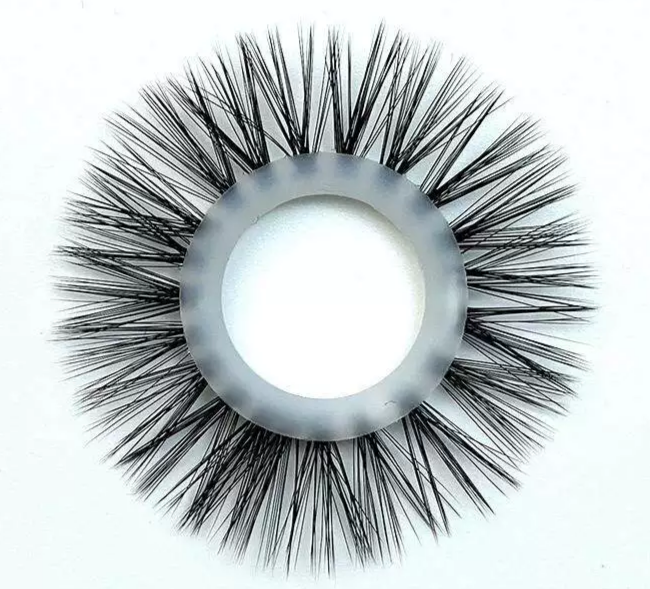
\includegraphics[width=0.5\textwidth]{images/fig_cockring.png}\\
{\footnotesize 图：羊眼圈（阴茎环）实物——环形结构，套于根部或冠状沟以维持硬度、延长勃起。}
\end{center}
\par\smallskip

\begin{itemize}[leftmargin=2em,itemsep=0.2em]
  \item \textbf{原理}：套在\textbf{阴茎根部或冠状沟}，靠压迫静脉、\textbf{减缓血液回流} → \textbf{维持硬度、延长勃起时间}；绒毛款在抽插时增加对伴侣的摩擦刺激。
  \item \textbf{关键定位}：它\textbf{只帮"维持已发生的勃起"，不能诱导勃起}——适合"能勃起但容易软"的人，\textbf{不是 ED 的一线治疗}（ED 首选仍是 PDE5 抑制剂，见 C 册）。
  \item \textbf{使用要点}：\textbf{勃起后套上更省力}；\textbf{配合水基 / 硅基润滑}别干磨；\textbf{别戴过夜 / 别超过 20--30 分钟不摘}（久压可致瘀滞、麻木）；出现\textbf{发白、发紫、刺痛、麻木立即取下}。
  \item \textbf{材质与清洁}：硅胶款\textbf{可沸水煮 3--5 分钟}；绒毛 / 天然皮毛款\textbf{只清洗不煮}（毛会脱落）；\textbf{一人一用、别共用}。
  \item \textbf{谁该慎用}：\textbf{对动物皮毛过敏、局部破损 / 炎症}别用天然款；\textbf{正在用抗凝血药、有色素沉着 / 血管脆弱者}别压太紧（呼应 C 册硝酸酯 × PDE5i 的血管管理逻辑）。
  \item \textbf{不避孕、不防病}——需要时仍要安全套。
\end{itemize}

\textbf{它和另外两类"延时"怎么分}\\
\begin{tabularx}{\textwidth}{@{}l X X@{}}
\toprule
\textbf{手段} & \textbf{机制} & \textbf{适用} \\
\midrule
环形 / 延时类（羊眼圈） & \textbf{物理}：压迫静脉减回流 & 能勃起但易软；配合伴侣的摩擦增强 \\
\midrule
延时喷剂 / 药膏 & \textbf{化学}：降低敏感度 & 敏感度偏高；注意别"麻到没感觉" \\
\midrule
Kegel 训练 & \textbf{肌肉}：加强盆底控制力 & 长期改善，可搭配上面两者 \\
\midrule
停 - 起始法 & \textbf{行为}：到临界点前暂停 & 最"零成本"，适合配合上面任一手段 \\
\bottomrule
\end{tabularx}

\subsection*{三、材质安全（接触黏膜的第一课）}
玩具接触黏膜（阴道/肛门/口腔），\textbf{材质比品牌更重要}：
\begin{tabularx}{\textwidth}{X l X}
\toprule
\textbf{材质} & \textbf{安全级} & \textbf{特点 / 注意} \\
\midrule
医用硅胶（platinum-cure） & \textbf{优} & 无孔、无毒、耐用；\textbf{别用硅基润滑}（腐蚀表面），别和 PVC 放一起（"串味"） \\
ABS 硬塑 & \textbf{优} & 无孔、安全、便宜；常见于振动棒外壳；可配任何润滑 \\
硼硅玻璃 & \textbf{优} & 无孔、可加温/冰镇；加温别超 45$^\circ$C、冰镇别低于 10$^\circ$C \\
不锈钢 & \textbf{优} & 无孔、可加温/冰镇、有重量感；同上温度注意 \\
TPE / TPR（软胶） & 良 & 软、便宜、有弹性；\textbf{多孔}藏菌、不宜共用、寿命短（1--2 年变粘） \\
PVC / 软质乙烯 & 慎用 & 便宜、常有刺鼻味；\textbf{多孔 + 可能含邻苯（塑化剂）}；避免长期/深入黏膜，若必须用\textbf{外覆安全套} \\
乳胶 & 良 & 有弹性；乳胶过敏者避免；\textbf{油基润滑会破坏乳胶} \\
\bottomrule
\end{tabularx}
\par\smallskip
\textbf{黄金规则}：首选\textbf{无孔材质}（医用硅胶/ABS/玻璃/金属，无孔 = 表面不藏菌 = 好清洗）；\textbf{避"软 + 有味道 + 便宜"}三样凑一起的（大概率 PVC/TPE）；看"body-safe"标识（不是认证，但代表厂家"知道该用什么"）。

\subsection*{四、润滑兼容（和材质一样重要）}
\begin{tabularx}{\textwidth}{X X X}
\toprule
\textbf{润滑类型} & \textbf{适用材质} & \textbf{注意事项} \\
\midrule
水基 & \textbf{所有材质} & 最安全、最通用；易干需补；与乳胶安全套兼容 \\
硅基 & 除硅胶外所有 & \textbf{不能用于硅胶玩具}（腐蚀表面）；持久耐水 \\
油基（凡士林/婴儿油/椰子油） & 除乳胶外 & \textbf{会破坏乳胶安全套}；阴道内易致菌群失衡、\textbf{不建议阴道内用}；肛交可用 \\
\bottomrule
\end{tabularx}
\par\smallskip
\textbf{速记}：硅胶玩具$\to$\textbf{水基}；玻璃/金属/ABS$\to$水基/硅基都行；TPE/TPR$\to$水基；肛交$\to$水基/硅基/油基都行（油基最持久）；和乳胶安全套用$\to$\textbf{水基/硅基}（油基会溶乳胶）。

\subsection*{五、清洁与消毒（最容易被忽视的"安全课"）}
\textbf{用前}：温水 + 中性肥皂/专用清洗液，\textbf{彻底冲洗干净}再用；检查表面有无裂痕/起皮/变粘（老化迹象）——有就换。
\textbf{用后}：\textbf{每次用完立即清洗}（别"攒下次"）；温水 + 中性肥皂\textbf{轻柔搓洗}（别用刷子猛刷划伤表面）；\textbf{彻底冲洗}（残留皂液刺激黏膜）；\textbf{自然晾干}（竖放/通风处，别用纸巾擦留纤维、别密封在盒里闷出细菌）。
\textbf{消毒加强}（共用/多人/肛交后）：
\begin{itemize}[leftmargin=2em,itemsep=0.2em]
  \item \textbf{无孔材质}（硅胶/玻璃/金属/ABS）：可\textbf{沸水煮 3--5 分钟}（确认耐热）或用 75\% 酒精擦拭。
  \item \textbf{有电机/电池的玩具}：\textbf{只擦不煮}（水会短路电机），用 75\% 酒精棉球擦表面。
  \item \textbf{TPE/TPR（多孔）}：\textbf{只擦不煮}（高温变形）；用后\textbf{套安全套}是最稳妥的隔离。
\end{itemize}
\textbf{存放}：干燥、通风、\textbf{别叠放}（表面接触会"粘"一起）；用\textbf{棉布袋}装（别用塑料袋）；避光、避高温（别放车里/暖气旁）。

\subsection*{六、共用与 STI 风险（别"想当然"）}
\textbf{核心原则}：玩具在两个人之间"换手/换部位"时，\textbf{必须清洗或换安全套}。
\begin{tabularx}{\textwidth}{X X X}
\toprule
\textbf{场景} & \textbf{风险} & \textbf{怎么做} \\
\midrule
A 用完直接给 B & 细菌/真菌/STI 交叉 & \textbf{清洗 + 干燥}后再用，或 A 用完\textbf{套个套子}再给 B \\
同一人：阴道$\to$肛门 & 肠道细菌$\to$尿路/阴道感染 & \textbf{必清洗或换套}（"从脏到干净"的顺序） \\
同一人：肛门$\to$阴道 & 同上、风险更高 & \textbf{必换套/清洗} \\
共用振动器（插入后换人） & HPV/疱疹/HIV 等 & \textbf{套隔离 + 清洗}，多孔材质尤其注意 \\
\bottomrule
\end{tabularx}
\par\smallskip
\textbf{为什么玩具能传 STI}：病毒/细菌可附着在玩具表面（多孔材质尤甚）；润滑液/体液会"锁住"病毒；\textbf{多孔材质的微孔能"藏"住病原体，清洗也洗不彻底}。
\textbf{最稳妥}：无孔材质 + 每次清洗 = 安全；多孔材质 + 每次套安全套 = 安全；多孔材质 + 不套不洗就换人 = 有风险。

\subsection*{七、选购深度指南（8 看 + 3 问）}
\textbf{8 看}：
\begin{enumerate}[leftmargin=2em,itemsep=0.2em]
  \item \textbf{看材质}：优先医用硅胶/ABS/玻璃/金属；避"未知软胶 + 刺鼻味"。
  \item \textbf{看认证/标识}：FDA（美）/CE（欧）/body-safe 是加分项（非必须，但代表厂家"知道该用什么"）。
  \item \textbf{看密封性}：防水（IPX7 以上）清洗更方便；不防水的\textbf{别泡水}（用湿布擦）。
  \item \textbf{看尺寸}：第一次选\textbf{中小号、单功能}；先入门再升级，别一步到位买"全家桶"。
  \item \textbf{看噪音}：振动类看分贝，\textbf{$<$50dB 更安静}；合租/隔音差优先静音款。
  \item \textbf{看充电/电池}：\textbf{USB 充电 $>$ 纽扣电池}（环保 + 方便 + 力度稳）；确认充电口防水。
  \item \textbf{看振动模式}：多模式比单频率灵活；但"模式多"不等于"好"，核心看力度和振幅。
  \item \textbf{看售后}：正规渠道、有退换、有保修；\textbf{别图便宜买"三无"}——黏膜接触的东西，便宜没好货是大概率。
\end{enumerate}
\textbf{3 问}（买前问自己）：
\begin{itemize}[leftmargin=2em,itemsep=0.2em]
  \item \textbf{"我穿/用它舒服吗？"}——不舒服的玩具，再贵也是负担。
  \item \textbf{"我想用多久？"}——偶尔用（月 1--2 次）和每天用，对材质/耐久度要求不同。
  \item \textbf{"我和伴侣都同意吗？"}——双人用的玩具，双方都舒服才用。
\end{itemize}

\subsection*{八、常见使用误区}
\begin{tabularx}{\textwidth}{X X}
\toprule
\textbf{误区} & \textbf{事实} \\
\midrule
"用玩具 = 伴侣不行" & 玩具是"加一只手"，不是"替代谁"，就像按摩器不替代手 \\
"振动越强越好" & 多数人 1--3 档就够；太强会\textbf{神经脱敏}，之后"怎么都不够" \\
"用一次就要'戒'" & 不需要"戒"，但\textbf{偶尔断档用回手指/嘴}，保持多感官参与 \\
"贵的 = 好的" & 不一定；200 元的医用硅胶振动棒可能比 800 元的"全功能"好用 \\
"不清洗也能用" & 黏膜接触 + 不清洗 = 细菌培养皿；\textbf{每次清洗是底线} \\
"肛塞不带底座也能用" & \textbf{不行}；直肠无尽头，不带底座可能滑入深处（需就医） \\
"硅胶玩具用硅基润滑没事" & \textbf{不行}；硅基会腐蚀硅胶表面（变粘/起皮/掉渣） \\
"玩具能'治'高潮障碍" & 不能；玩具是增强工具，不是治疗手段；持续障碍需就医 \\
"用玩具 = 自慰" & 不一定；伴侣间用、双人穿戴、APP 遥控都是"亲密互动"的一部分 \\
"玩具只有'那个部位'能用" & 不对；振动棒可刺激乳晕/颈/耳后/脊柱，按摩棒可按摩肩/背/腿——\textbf{全身都是"敏感区"} \\
\bottomrule
\end{tabularx}

\subsection*{九、进阶与特殊需求}
\begin{itemize}[leftmargin=2em,itemsep=0.4em]
  \item \textbf{温度玩法}：玻璃/金属可\textbf{加温或冰镇}（37--45$^\circ$C 或 10--15$^\circ$C）增加温度变化刺激；别用普通蜡烛（熔点太高烫伤），用\textbf{专用体温蜡烛}（熔点约 37$^\circ$C）；加温/冰镇前确认材质耐热/耐寒（TPE/TPR 不耐极端温度）。
  \item \textbf{APP/遥控}：适合异地/角色扮演/"惊喜"场景；\textbf{提前测试信号稳定性}（蓝牙范围、APP 兼容）；\textbf{关手机通知}。
  \item \textbf{多人/群体}：每人\textbf{自带玩具}最安全（避免共用）；必须共用时，\textbf{无孔材质 + 每次清洗/换套}。
  \item \textbf{敏感度低/需要强刺激}：试\textbf{大型按摩棒（wand）}（力度强、面积大）或\textbf{吮吸类（air pulse）}（非接触，对"怕摩擦但需强刺激"的人友好）；配合\textbf{盆底肌训练}（见本册《享受高潮》章"呼吸与盆底"一节）——肌肉强 = 敏感度更好。
\end{itemize}

\subsection*{一页要点}
情趣玩具 = \textbf{感官刺激的物理增强工具}，不是替代品、不是药、不挑性别取向。
\begin{itemize}[leftmargin=2em,itemsep=0.2em]
  \item \textbf{六大类}：振动类（阴蒂/G 区/前列腺，最入门）/ 插入类（体积/充实感）/ 穿戴类（双人同步）/ 辅助类（前戏感官增强）/ \textbf{男性自慰器具（飞机杯/名器/炮机，男用"杯"进阶梯度）}/ \textbf{仿真人偶（充气娃娃/实体娃娃/阴道倒膜）}。\textbf{另有"环形/延时类"（羊眼圈，阴茎环）}——对着冠状沟/根部的功能性进阶，见"二·附、部位进阶"第 4 条。
  \item \textbf{材质是第一课}：医用硅胶/ABS/玻璃/金属（无孔、安全）$>$ TPE/TPR（多孔、短寿）$>$ PVC（慎用）。
  \item \textbf{润滑兼容}：硅胶玩具配\textbf{水基}；玻璃/金属配水基/硅基都行；\textbf{别用油基 + 乳胶安全套}。
  \item \textbf{清洁是底线}：每次用完洗、自然晾干、无孔材质可煮沸、多孔材质只擦 + 套隔离。
  \item \textbf{共用规则}：换人/换部位必清洗或换套；阴道$\to$肛门$\to$阴道必换套。
  \item \textbf{使用要点}：从最低档开始、配合润滑、位置可移动、别只依赖（偶尔断档用回手指）。
  \item \textbf{肛塞必带底座}（直肠无尽头）；\textbf{硅胶玩具别用硅基润滑}（会腐蚀）。
  \item \textbf{选购 8 看 + 3 问}：材质/认证/密封/尺寸/噪音/充电/模式/售后；舒服吗？用多久？双方同意吗？
  \item \textbf{常见误区}：振动不是越强越好、玩具不是"伴侣不行"、清洗不是"可选"。
\end{itemize}

\section{情趣内衣：完整介绍}

\subsection*{先定调：它到底是什么}
情趣内衣的核心作用是\textbf{视觉刺激 + 心理唤起}——让"看到对方"这件事本身变成唤起的一部分。它对双方都有效（不只是女性穿给男性看），也不是"必需品"或"考试道具"。
先放下三个常见误区：
\begin{itemize}[leftmargin=2em,itemsep=0.3em]
  \item \textbf{不是"不穿就不够性感"}：裸体、运动服、甚至一件旧 T 恤都能唤起人，取决于关系质量和氛围，不取决于布料的多少。
  \item \textbf{不是"女性专属"}：男性情趣内衣（网眼背心、皮质短裤、吊带袜等）同样存在，双方都可以选。
  \item \textbf{不是"一次性的"}：不必每次"有需求"就穿，也不必每次都不穿——\textbf{双方都觉得舒服、想穿就穿}才是正解。
\end{itemize}

\subsection*{常见类型与适用场景}
\begin{tabularx}{\textwidth}{X X X X}
\toprule
\textbf{类型} & \textbf{特点} & \textbf{适合场景} & \textbf{注意} \\
\midrule
蕾丝套装（文胸+内裤/吊带） & 经典款、半透明、强调线条 & 纪念日、约会、想"正式一点" & 蕾丝可能磨皮肤，敏感肌选棉底 \\
连体内衣（bodysuit） & 一体式、强调全身线条 & 想"整体感"、视觉展示 & 注意裆部是否可开（方便洗手间） \\
透明/网纱款 & 大面积透视、若隐若现 & 高唤起场景、双方都爱"看" & 内层最好有衬里（防走光+舒适） \\
系带/绑带款（strappy） & 细带交叉、结构感强 & 想"设计感"、偏 Kink 入门 & 带子别太细/太紧，会勒痕 \\
运动风（运动内衣+短裤） & 功能面料、健康活力 & 日常、运动后、"不经意"的吸引 & 最舒适，适合第一次尝试 \\
角色扮演款（女仆/护士/制服） & 主题明确、配合对话 & 想"换换心情"、配合角色 & 角色+对话才有效，别只看款式 \\
吊带袜/长筒袜 & 单穿也成立、"加一件" & 最轻量的变化 & 注意防滑脱（硅胶条/吊带） \\
简约纯色款（缎面/丝质） & 低刺激、高级感 & 日常、不想"太用力" & 最百搭，适合"不确定穿什么"时 \\
\bottomrule
\end{tabularx}
\par\smallskip
\textbf{选择原则}：第一次选\textbf{低刺激款}（运动风/简约纯色/吊带袜），别一步到位上"全套蕾丝+绑带+眼罩"——\textbf{唤起是渐进的，不是开关}。

\begin{center}

\includegraphics[width=0.5\textwidth]{images/fig_lingerie_style.png}\\
{\footnotesize 图：情趣内衣款式实物——覆盖上表多类（蕾丝/系带/连体等），供选型时对照"低刺激款优先"原则。}
\end{center}
\par\smallskip

\subsection*{材质详解（穿在身上的安全课）}
\begin{tabularx}{\textwidth}{X l l X X}
\toprule
\textbf{材质} & \textbf{触感} & \textbf{透气} & \textbf{适合谁} & \textbf{注意} \\
\midrule
真丝/桑蚕丝 & 滑、凉、高级 & 中 & 不敏感、追求质感 & 贵、需手洗，别用烘干机 \\
蕾丝（化纤） & 微刺、有弹性 & 低 & 不敏感 & 久穿闷热，超过 2 小时换下 \\
棉混纺（棉+氨纶） & 软、贴肤 & 高 & \textbf{敏感肌首选} & 最舒服、最透气 \\
莫代尔 & 丝滑、垂坠 & 中高 & 追求舒适+外观 & 性价比好 \\
网纱/欧根纱 & 硬、有骨架感 & 高 & 追求"结构" & 别直接贴皮肤（加衬里） \\
缎面（涤纶） & 滑、有光泽 & 低 & 追求"光感" & 闷热，夏天慎用 \\
皮质/PU 皮 & 硬、有型 & 低 & 偏 Kink/视觉展示 & 透气差，别穿超过 1 小时 \\
\bottomrule
\end{tabularx}
\par\smallskip
\textbf{黄金规则}：\textbf{贴皮肤的那一层，优先选棉/莫代尔/真丝}；外面那层（蕾丝/网纱/缎面）负责"好看"。两层分工，舒适和颜值兼得。

\subsection*{尺码：不是 S/M/L 一刀切}
情趣内衣的尺码和日常内衣\textbf{完全不同}，尤其连体款和系带款：
\begin{enumerate}[leftmargin=2em,itemsep=0.2em]
  \item \textbf{看具体尺寸表}：正规品牌会给胸围/腰围/臀围/身高的对照表，\textbf{不是"你平时穿 M 就买 M"}。
  \item \textbf{量三个数}：用软尺量\textbf{下胸围}（不是上胸围）、\textbf{最细腰围}、\textbf{最宽臀围}，对照表选。
  \item \textbf{连体内衣多量一个}：裆部到腋下的长度（影响裆部是否开档）。
  \item \textbf{宁大勿小}：偏小会勒、偏大会松垮——\textbf{偏小比偏大更影响体验}（勒痕+不透气+不舒服）。
  \item \textbf{系带款看"可调节范围"}：松紧范围越大，容错越高。
  \item \textbf{第一次买}：选\textbf{自己日常尺码或大半号}，别"挑战小一号"。
\end{enumerate}

\subsection*{颜色与心理暗示}
颜色不只是"好看"，它传递的信号不同：
\begin{tabularx}{\textwidth}{X X X}
\toprule
\textbf{颜色} & \textbf{常见暗示} & \textbf{适合场景} \\
\midrule
黑色 & 经典、神秘、"万能" & 任何场景，最安全的选择 \\
红色 & 热情、直接、"今晚有戏" & 纪念日、想"主动" \\
白色 & 纯净、反差感（尤其配深色皮肤） & 想"反差"、婚纱/婚礼主题 \\
肤色/裸色 & 若隐若现、"像没穿" & 想"自然"但不想全裸 \\
透明/裸色+花纹 & 强调线条、若隐若现 & 高唤起场景 \\
撞色/印花 & 活泼、年轻、"不严肃" & 日常、想轻松 \\
\bottomrule
\end{tabularx}
\par\smallskip
\textbf{没有"最性感的颜色"}——取决于对方的偏好和你们的默契。第一次不确定？\textbf{黑色最稳}。

\subsection*{搭配与场景（实操）}
\begin{itemize}[leftmargin=2em,itemsep=0.4em]
  \item \textbf{场景 1：日常"不经意"}——日常内衣外面套一件宽松衬衫/T 恤，若隐若现。重点是"自己穿得舒服，对方恰好看到了"，压力最小、效果最好。适合不想"太用力"的日子。
  \item \textbf{场景 2：纪念日 / 约会}——完整套装（文胸+内裤/连体），搭配鞋包。仪式感来自"你精心准备了"，不来自布料多少。配合前戏完整剧本的氛围段（暖光、音乐、慢节奏），别"一进门就脱光"——让对方"看"的过程本身是唤起。
  \item \textbf{场景 3：角色扮演 / 主题夜}——主题款（女仆/护士/运动风）+ 配合对话和剧本（"今天你是我的教练"）。\textbf{角色大于服装}——一件普通运动背心 + "今天我是你的私人教练"的对话，比昂贵女仆装 + 尬聊有效得多。
  \item \textbf{场景 4：单件加搭（最轻量）}——日常内衣 + 一双吊带袜 / 一条蕾丝腰带 / 一副袖套，只加一件、不换一身。最轻量的"变化"，压力最小。
\end{itemize}

\subsection*{穿着舒适度（被忽略的关键）}
再好看的款式，\textbf{穿着不舒服就全废了}——注意力会从"享受"转移到"这带子勒得我疼"：
\begin{itemize}[leftmargin=2em,itemsep=0.3em]
  \item \textbf{透气}：连续穿超过 2 小时会闷，选棉/莫代尔内衬；蕾丝/缎面外搭可以，别贴身。
  \item \textbf{不勒}：系带款松紧以"能伸进两指"为准；连体款肩带别太细。
  \item \textbf{不滑脱}：吊带袜选\textbf{带硅胶防滑条}的；连体款选\textbf{肩带可调节}的。
  \item \textbf{裆部}：连体款最好选\textbf{可开裆}的（方便洗手间，不用"忍着"）。
  \item \textbf{缝线}：内侧缝线要\textbf{平整、无毛刺}——贴皮肤的地方有粗糙缝线，等于持续摩擦刺激。
  \item \textbf{试穿}：\textbf{在家先穿 10 分钟}，走动、弯腰、坐下，确认不会滑脱/勒/卡——别到了"正事"才发现不舒服。
\end{itemize}

\subsection*{卫生与护理}
\begin{itemize}[leftmargin=2em,itemsep=0.3em]
  \item \textbf{首次穿着前清洗一次}：去除染料、甲醛、工业残留。冷水 + 中性洗涤剂，\textbf{别用热水}（会缩水/掉色）。
  \item \textbf{每次使用前后清洗}：贴身衣物不共用、不隔夜。
  \item \textbf{单独洗}：别和袜子、毛巾混洗；蕾丝/真丝\textbf{手洗}，别机洗（会勾丝）。
  \item \textbf{存放}：干燥、通风、\textbf{别用塑料袋密封}（会闷出味道）；蕾丝/真丝用\textbf{棉布袋}装，别直接叠硬盒里（会压痕）。
  \item \textbf{别"一次买穿三年"}：再贵的真丝，穿着次数多了也会起球/变形/褪色——\textbf{这是正常的，不是质量问题}。
\end{itemize}

\subsection*{选购避坑}
\begin{tabularx}{\textwidth}{X X}
\toprule
\textbf{坑} & \textbf{怎么避} \\
\midrule
只看图不看材质标 & 翻到标签看成分：棉/丝/蕾丝比例；"95\% 尼龙 5\% 氨纶"和"60\% 棉 40\% 蕾丝"手感完全不同 \\
信"均码" & 情趣内衣几乎没有"均码"——看具体尺寸表 \\
图与实物色差大 & 看买家秀、别只看模特图；选支持 7 天无理由退换的渠道 \\
"越贵越好？" & 不一定——200 元的棉混纺可能比 800 元的"全蕾丝"舒服；舒适优先于价格 \\
一次买一整套 & 第一次先买单件（吊带袜/蕾丝腰带），确认喜欢再升级 \\
只看"性感度" & 问自己："我穿着它舒服吗？想穿多久？"——答案比"看起来多性感"重要 \\
渠道 & 优选品牌官网/正规电商旗舰店；避"三无"地摊款（染料/甲醛/缝线无保障） \\
\bottomrule
\end{tabularx}

\subsection*{双方沟通与意愿}
\begin{itemize}[leftmargin=2em,itemsep=0.3em]
  \item \textbf{别"惊喜式"强加}：一方精心准备、另一方觉得"没必要"——都不丢人。"我想试试，你觉得呢？"比"你看我穿了什么"压力小得多。
  \item \textbf{穿给谁看、什么时候穿、穿多不穿}——双方都可以拒绝，也都可以提要求，不需要"配合"。
  \item \textbf{别拿情趣内衣当"考核"}：穿了好看 = 你满意；穿了不好看 = 也正常，\textbf{人的身体没有标准答案}。
  \item \textbf{如果对方不想穿}：尊重。"不穿也很好"是完全成立的——\textbf{唤起的核心是关系质量和氛围，不是一件 200 块的蕾丝}。
\end{itemize}

\subsection*{一页要点}
情趣内衣 = \textbf{视觉与心理唤起工具}，不是必需品、不是考核、不挑性别。
\begin{itemize}[leftmargin=2em,itemsep=0.2em]
  \item \textbf{类型}：蕾丝套装 / 连体 / 透明 / 系带 / 运动风 / 角色扮演 / 吊带袜 / 简约纯色——\textbf{第一次选低刺激款}。
  \item \textbf{材质}：贴皮肤层选棉/莫代尔/真丝（舒适）；外搭层选蕾丝/缎面/网纱（好看）。\textbf{舒适优先于颜值，颜值优先于价格}。
  \item \textbf{尺码}：量下胸围/腰围/臀围，看具体尺寸表，\textbf{宁大勿小}。
  \item \textbf{颜色}：黑色最稳、红色最热情、白色反差感，\textbf{没有"最性感"的颜色}。
  \item \textbf{搭配}：日常不经意 / 纪念日仪式 / 角色扮演配合对话 / 单件加搭最轻量。
  \item \textbf{舒适}：透气（别穿超过 2 小时）、不勒、不滑脱、裆部可开、缝线平整、\textbf{在家先试穿 10 分钟}。
  \item \textbf{卫生}：首次洗、每次洗、单独洗、通风存、别塑料袋密封。
  \item \textbf{沟通}：双方自愿、可以拒绝、别当考核——\textbf{关系质量和氛围优先于一件蕾丝}。
\end{itemize}

\section{选购避坑清单（一页速查）}
\begin{enumerate}[leftmargin=2em,itemsep=0.2em]
  \item \textbf{看材质}：优先医用硅胶/ABS/玻璃/金属；避"未知软胶+刺鼻味"。
  \item \textbf{看认证}：优选有 FDA（美）/CE（欧）标识或"body-safe"标注的；\textbf{没认证不等于不安全，但认证是加分项}。
  \item \textbf{看密封性}：防水（IPX7）的清洗更方便；\textbf{不防水的别泡水里洗}。
  \item \textbf{看尺寸}：第一次选\textbf{中小号、单功能}；先入门再升级，别一步到位买"全家桶"。
  \item \textbf{看噪音}：振动类看分贝（dB），\textbf{<50dB 更安静}；合租/家庭隔音差优先静音款。
  \item \textbf{看充电/电池}：\textbf{USB 充电 > 纽扣电池}（环保+方便）；确认充电口防水。
  \item \textbf{看售后}：正规渠道、有退换；\textbf{别图便宜买"三无"}——黏膜接触的东西，便宜没好货是大概率。
  \item \textbf{情趣内衣}：看\textbf{成分标}（棉/丝/蕾丝比例）、\textbf{尺码表}（不是 S/M/L 一刀切）、\textbf{是否可机洗}。
\end{enumerate}

\section{一页要点}
情趣用品 = \textbf{可选的愉悦增强工具}，不是必需品、不是补救药、不挑性别取向。
\textbf{材质安全是第一课}：医用硅胶/ABS/玻璃/金属 > 软胶；\textbf{硅胶玩具别配硅基润滑}。
\textbf{清洁和共用规则}比"买什么"更重要：用前后清洗、换人/换部位必换套、多孔材质别共用。
情趣内衣 = \textbf{视觉与心理唤起}，舒适 > 好看，双方自愿 > 标准答案。
选购记住"材质/认证/尺寸/噪音/充电/售后"六看。


\chapter{润滑剂与保湿剂：成分、选购、保存与兼容}

\begin{center}
\myhei\large 润滑剂用对是"加分"，用错是"减分"——成分、材质、安全套三者要一起看
\end{center}

\section{先分清三个概念}
\begin{itemize}[leftmargin=2em,itemsep=0.3em]
  \item \textbf{润滑剂（lubricant）}：性生活\textbf{当时}用的，减少摩擦、增加舒适，用完即弃（水基/硅基/油基）。
  \item \textbf{阴道保湿剂（moisturizer）}：\textbf{日常}用的，缓解长期干涩，隔天或每天用（成分与润滑剂不同）。
  \item \textbf{局部药物}：医生开的\textbf{局部雌激素/激素}，用于激素性干涩（如绝经后），\textbf{需就医}，不是"润一润"。
\end{itemize}
三者目的不同，\textbf{别混用、别指望一个解决另一个的问题}。

\section{四大类成分详解}
\begin{tabularx}{\textwidth}{X X X}
\toprule
\textbf{类型} & \textbf{特点} & \textbf{适合场景 / 注意} \\
\midrule
水基 & 易清洗、通用、与乳胶安全套兼容 & \textbf{最常用、最安全}；易干需补；\textbf{含甘油的敏感者慎选} \\
硅基 & 持久、耐水、可配水/油外材质 & \textbf{不能用于硅胶玩具}（腐蚀）；肛交、水下场景好；洗需肥皂 \\
油基（凡士林/椰子油等） & 持久、便宜 & \textbf{会溶乳胶安全套}；阴道内易致菌群失衡、不建议；肛交可用 \\
特殊（含味/含麻/含辣） & 增加趣味/局部麻刺感 & 多为\textbf{水基+添加剂}；\textbf{敏感/破损黏膜慎用}；麻/辣含活性成分，先小面积试 \\
\bottomrule
\end{tabularx}

\section{敏感成分速查（看标签）}
\begin{tabularx}{\textwidth}{X X}
\toprule
\textbf{成分} & \textbf{对谁不友好} \\
\midrule
甘油（glycerin） & 易致\textbf{酵母菌（念珠菌）}过度生长——反复发作的"霉菌"人群少用 \\
丙二醇（propylene glycol） & 少数人\textbf{刺激/过敏}；敏感肌可选"无丙二醇"款 \\
香精 / 香味 & \textbf{刺激黏膜}，敏感者、阴道内使用尽量避免 \\
paraben（对羟基苯甲酸酯） & 争议成分，敏感者可选"无 paraben" \\
苯扎氯铵等杀菌剂 & \textbf{刺激性强}，黏膜反复用易不适 \\
\bottomrule
\end{tabularx}
\par\smallskip
\textbf{敏感体质 / 反复炎症}：选\textbf{无甘油、无香精、无 paraben、pH 接近 4.5}（阴道）的"温和配方"，并优先咨询医生。

\section{选购避坑}
\begin{itemize}[leftmargin=2em,itemsep=0.3em]
  \item \textbf{先问用途}：阴道内 / 肛交 / 口交 / 配合玩具 / 配合安全套——不同用途首选不同。
  \item \textbf{看成分表前 5 位}：甘油、香精排前面且你是敏感体质，慎选。
  \item \textbf{"含麻/含辣/升温"是功能款}：不是人人适合，\textbf{先小面积试、别空腹、破损皮肤别用}。
  \item \textbf{避"三无+刺鼻味+很便宜"}：黏膜接触的东西，成分无保障风险高。
  \item \textbf{别"一管用到过期"}：看生产日期和保质期（未开封一般 2--3 年，开封后建议 3--6 个月内用完）。
\end{itemize}

\section{保存期与失效判断}
\begin{itemize}[leftmargin=2em,itemsep=0.3em]
  \item \textbf{未开封}：避光、避高温（别放车里/暖气旁），一般 2--3 年。
  \item \textbf{开封后}：水基建议 3--6 个月、硅基可稍长；\textbf{每次用完盖紧}，避免沾手带入细菌。
  \item \textbf{失效信号}：变色、变稠/变稀、异味、分层、结块——\textbf{出现任一就换}。
  \item \textbf{分装小瓶}：旅行用\textbf{干净小瓶分装}（先洗手），别直接从大管"挤一点"（管口反复沾手）。
\end{itemize}

\section{「润滑 × 材质 × 安全套」三方兼容矩阵（核心）}
\begin{tabularx}{\textwidth}{X X X X}
\toprule
\textbf{润滑} & \textbf{乳胶安全套} & \textbf{硅胶玩具} & \textbf{玻璃/金属/ABS 玩具} \\
\midrule
水基 & \textbf{可用} & \textbf{可用} & \textbf{可用} \\
硅基 & \textbf{可用} & \textbf{不可用}（腐蚀） & \textbf{可用} \\
油基 & \textbf{不可用}（溶乳胶） & \textbf{可用} & \textbf{可用} \\
\bottomrule
\end{tabularx}
\par\smallskip
\textbf{一句话速记}：\textbf{拿不准就用"水基 + 乳胶安全套"}——它几乎通吃所有组合；只有"硅胶玩具"要避开硅基。

\section{阴道保湿剂（干涩的长期方案）}
\begin{itemize}[leftmargin=2em,itemsep=0.3em]
  \item \textbf{什么时候用}：润滑剂是"当时用"，保湿剂是\textbf{"平时用"}——干涩持续（尤其绝经后、哺乳后、激素波动）时，单靠润滑不够，\textbf{保湿剂打底 + 必要时润滑}才是组合拳。
  \item \textbf{怎么选}：同样看成分（避甘油/香精/paraben）；选\textbf{pH 温和、无刺激}款。
  \item \textbf{效果有限时就医}：若保湿+润滑仍干涩疼痛，可能是\textbf{激素性（绝经/产后）或盆底问题}，看妇科，局部雌激素是循证一线（见 D 册）。
\end{itemize}

\section{性前/性后清洁与卫生（来自旧书"性卫生"精华）}

\textbf{性前清洁（双方）}：

\begin{itemize}[leftmargin=2em,itemsep=0.3em]
  \item \textbf{男性}：用温水 + 温和清洗液清洗阴茎和阴囊；\textbf{翻开包皮清洗冠状沟}（包皮垢是细菌和刺激源）；清洗后擦干。
  \item \textbf{女性}：用温水清洗外阴（大小阴唇、阴蒂周围）；\textbf{顺序：从前向后}（先阴部、再肛门），防止肠道细菌带入；\textbf{不要冲洗阴道内部}（阴道自洁系统，冲洗反而破坏菌群）。
  \item 清洗后\textbf{彻底擦干}，尤其腹股沟褶皱处。
\end{itemize}

\textbf{性后清洁}：

\begin{itemize}[leftmargin=2em,itemsep=0.3em]
  \item 双方再次清洗外生殖器（温水即可，不必用特殊药剂）。
  \item \textbf{女性排尿}——尿液冲刷尿道，显著降低 UTI 风险（尤其"性交后膀胱炎"）。
  \item 不必每次性后都用杀精剂或药物清洗——\textbf{过度清洁反而破坏微生态}。
\end{itemize}

\textbf{时机与环境（旧书"性差异与性卫生"精华）}：

\begin{itemize}[leftmargin=2em,itemsep=0.3em]
  \item \textbf{不要在极度疲劳时进行}——身心疲惫时质量和满意度都会下降；先休息 15--30 分钟再开始。
  \item \textbf{环境要点}：安静、不被打扰、温度舒适；\textbf{不必全黑}——柔和的暖光/彩色灯有助于集中感官。
  \item \textbf{床品整洁舒适}——这是"仪式感"的一部分，影响心理放松。
\end{itemize}

\textbf{日常卫生补充（旧书"男性/女性性器官卫生"精华）}：

\begin{itemize}[leftmargin=2em,itemsep=0.3em]
  \item \textbf{男性包皮垢}：包皮和龟头之间的腺体分泌物 + 尿渍 = "包皮垢"；长期堆积可致发炎、刺激伴侣、甚至增加宫颈癌风险——\textbf{每日翻开清洗是基本操作}。
  \item \textbf{女性五期注意}：经期（勤换、不冲洗）、孕期（更温和的清洁）、产褥期（从前向后、保持干燥）、哺乳期（注意清洁防感染）、绝经期（干涩时加保湿剂）。
  \item \textbf{内裤单独洗}：不与袜子/外衣同洗；阳光晾干；避免阴冷潮湿处存放。
  \item \textbf{不要滥用阴道冲洗}：除非医嘱，否则"温水 + 外部清洗"足够了。
\end{itemize}

\section{一页要点}
润滑剂 = \textbf{当时用}、保湿剂 = \textbf{平时用}、局部药物 = \textbf{就医用}，三者别混。
\textbf{成分三看}：甘油（易致霉菌）、香精（刺激）、pH（阴道选近 4.5）——敏感体质选"无甘油/无香精/无 paraben"温和款。
\textbf{兼容核心}：拿不准就用\textbf{水基 + 乳胶安全套}（几乎通吃）；\textbf{硅胶玩具避开硅基}；油基会溶乳胶。
\textbf{保存}：开封后水基 3--6 个月内用完；变色/异味/分层就换；旅行用干净小瓶分装。


\chapter{收纳、清洁与旅行}

\begin{center}
\myhei\large 工具的价值，一半在使用、一半在"养"——干净、干燥、分装好，寿命和安全性都翻倍
\end{center}

\section{专用清洁：选对"洗"这一步}
\begin{itemize}[leftmargin=2em,itemsep=0.3em]
  \item \textbf{日常清洗}：温水 + \textbf{中性肥皂}或专用清洗液即可；\textbf{别用洗洁精/酒精长时间泡}（伤材质、残留刺激）。
  \item \textbf{杀菌喷雾/清洗液}：含温和杀菌成分（如苯扎氯铵低浓度）的\textbf{外出/共用}后喷一喷方便；\textbf{别天天喷}（过度杀菌反而刺激）。
  \item \textbf{消毒分级}：\textbf{无孔材质}（硅胶/玻璃/金属）可\textbf{沸水煮 3--5 分钟}；有电机/电池的\textbf{只擦不煮}；多孔材质\textbf{只擦 + 套隔离}。
  \item \textbf{清洗工具}：软布/海绵 > 刷子（刷子易划伤表面藏菌）；清洗后\textbf{自然晾干}再收纳。
\end{itemize}

\section{收纳：防潮、防串味、防"粘"}
\begin{itemize}[leftmargin=2em,itemsep=0.3em]
  \item \textbf{干燥是底线}：湿着收 = 闷出细菌/霉味；\textbf{彻底晾干}再装。
  \item \textbf{用布袋，别用塑料袋}：棉/无纺布袋透气；塑料袋闷、不透气、材质还易"串味"。
  \item \textbf{分开放}：不同玩具\textbf{各装一袋}，别叠一起（表面接触会"粘"、也避免材质间"串味"，尤其硅胶别和 PVC 放一起）。
  \item \textbf{避光避高温}：别放车里、暖气旁、阳光直射——加速材质老化。
  \item \textbf{电池/电量}：长期不用的电动玩具\textbf{取出电池或保持半电}，避免过放；充电款别"满电吃灰"。
\end{itemize}

\section{旅行与便携}
\begin{itemize}[leftmargin=2em,itemsep=0.3em]
  \item \textbf{便携装}：选\textbf{小体积、可密封}的款式；电动玩具确认\textbf{有"旅行锁"}（防包里误按开机）。
  \item \textbf{润滑剂分装}：干净小瓶装（先洗手），\textbf{航空携带注意 100ml 液体规定}——超了放托运。
  \item \textbf{酒店场景}：带\textbf{一次性清洁湿巾/杀菌喷雾}（酒店洗手液未必温和）；\textbf{用完当地洗不放心就喷 + 晾干}再收。
  \item \textbf{隐私}：收纳袋/盒子\textbf{不透明}，避免"一眼看穿"的尴尬。
  \item \textbf{清洁随身}：\textbf{免洗洗手液 + 一次性手套}（共用前临时隔离）是很实用的旅行组合。
\end{itemize}

\section{一页要点}
清洁 = \textbf{温水 + 中性肥皂/专用液}，无孔可煮沸、有电机只擦、多孔只擦+套隔离；\textbf{别用洗洁精/酒精久泡}。
收纳 = \textbf{干燥、布袋、分开放、避光避高温}；硅胶别和 PVC 放一起。
旅行 = \textbf{便携装 + 旅行锁 + 分装小瓶 + 杀菌喷雾}；航空液体 100ml 规定；带一次性清洁湿巾和手套最实用。


\chapter{欲望不匹配：高低欲伴侣怎么办}

\begin{center}
\myhei\large 欲望差很多，多半不是"谁不够爱"，而是节奏、时机、强度三件事没对齐
\end{center}

\section{先正名：欲望差异是正常变异}
"谁想要得多、谁想要得少"在伴侣中\textbf{极其普遍}，且\textbf{不随时间必然收敛}。它不是"谁的错"、不是"不爱了"、也不是"性冷淡"，而是两个人\textbf{生理节奏 + 情绪状态 + 生活压力}的自然差异。
先把这句话收下：\textbf{高欲不代表"更正常/更主动"，低欲也不代表"有问题/不够投入"——双方都有正当性。}

\section{区分三种"不匹配"（对症下药）}
\begin{tabularx}{\textwidth}{X X X}
\toprule
\textbf{类型} & \textbf{表现} & \textbf{核心症结} \\
\midrule
频率差异 & 一方想要 5 次/周、另一方 1 次/周 & \textbf{节奏/时机}没对齐，不是"要不要" \\
时机差异 & 一方在睡前、另一方在周末 & \textbf{日程/触发点}不同 \\
强度差异 & 一方想要"重一点"、另一方想要"轻一点" & \textbf{偏好/强度}不同（与欲望量无关） \\
\bottomrule
\end{tabularx}
\par\smallskip
\textbf{先分清是哪一种}，再谈"怎么办"——把"频率差异"误当成"强度差异"（或反之），沟通就会跑偏。

\section{沟通框架（怎么开口不吵架）}
\begin{enumerate}[leftmargin=2em,itemsep=0.3em]
  \item \textbf{用"我想要"而非"你怎么不"}：\textbf{"我最近很想要我们多亲密一些" > "你最近对我没兴趣"}。
  \item \textbf{先听后说}：低欲一方常说"我没感觉"，高欲一方常想"你是不是不爱我"——\textbf{先让对方把"没感觉"背后的压力/疲惫/状态说完}，再谈方案。
  \item \textbf{把"性"拆成可谈的小项}：频率、时机、强度、方式，\textbf{逐项对齐}，别 lump 成"我们要不要做"一个开关。
  \item \textbf{定一个"双方都不亏"的节奏}：不是各退半步（5 次 vs 1 次 $\to$ 3 次，双方都不满意），而是\textbf{找到"高欲方觉得够、低欲方不勉强"的落点}（可能是 2 次 + 更多非插入亲密）。
  \item \textbf{定期复盘}（每月一次，5 分钟）：\textbf{"这个节奏你舒服吗？想调整吗？"——别等矛盾攒到爆才谈}。
\end{enumerate}

\section{工具与调节（不是"将就"，是"扩展菜单"）}
\begin{itemize}[leftmargin=2em,itemsep=0.3em]
  \item \textbf{自慰分担}：高欲方\textbf{部分需求自己满足}（玩具/手指），低欲方不觉得"每次都要配合"——\textbf{这是最常被低估的减压阀}。
  \item \textbf{玩具/穿戴类}：双方同步、或一方主导的\textbf{"半参与"亲密}（如穿戴式振动器），降低"必须全程投入"的压力。
  \item \textbf{远程/数字性爱}：见本册《远程与数字性爱》章——\textbf{不在同一空间时的亲密补充}。
  \item \textbf{非插入亲密}：拥抱、亲吻、按摩、一起泡澡——\textbf{"亲密"不等于"插入"，低欲方往往对"非插入亲密"接受度更高}。
  \item \textbf{固定"亲密窗口"}：比如"周五晚上"作为双方预期内的亲密时间，\textbf{降低"随机被要求"的抗拒感}。
\end{itemize}

\section{别踩的坑}
\begin{itemize}[leftmargin=2em,itemsep=0.3em]
  \item \textbf{把欲望当 KPI}：高欲方"没达到次数就失落"、低欲方"每次都像在完成任务"——\textbf{两个都累}。
  \item \textbf{愧疚感绑架}：低欲方觉得"是我不够好"、高欲方觉得"是我要求太多"——\textbf{都不是}，这是差异。
  \item \textbf{冷战 / 突然热情}：低欲方"攒大招"（平时不接、突然某天很主动）、高欲方"赌气式冷淡"——\textbf{都伤关系}。
  \item \textbf{把"低欲"当"性冷淡"去"治"}：多数低欲是\textbf{正常变异}，不是病；\textbf{别一有差异就"就医"}。
\end{itemize}

\section{常见烦恼速查（来自旧书"解决你的疑问"精华）}

以下按"问题→为什么→怎么办"格式整理，覆盖最常被问到的 8 类困扰：

\begin{tabularx}{\textwidth}{@{}X X X@{}}
\toprule
\textbf{烦恼} & \textbf{为什么会出现} & \textbf{怎么办（实操）} \\
\midrule
\textbf{太干涩} & 唤起不足/激素变化/润滑剂不够；$\ne$ "没性欲" & 延长前戏 + 使用水基/硅基润滑；不必不好意思 \\
\midrule
\textbf{放屁声} & 插入时带入空气，必然排出；某些体位（如女上/后入）更明显 & 一笑置之；换体位可减轻；\textbf{这不是"不干净"} \\
\midrule
\textbf{伴侣"乏味"} & 固定流程、缺少变化、沟通断裂 & 主动提出新尝试；角色扮演/新位置/新时间；\textbf{不要等对方来"创新"} \\
\midrule
\textbf{双方都"没感觉"} & 疲劳/压力/药物/季节/生活节奏；$\ne$ "不爱了" & 折衷：非插入亲密（口交/爱抚/玩具）；降低频率但提高质量；先排除生理因素 \\
\midrule
\textbf{讨厌自己身体} & 社会审美标准 + 与伴侣初期的"滤镜"消退 & 停止在过程中"审视自己"；关注"感受"而非"外观"；\textbf{你的感受 > 你的形象} \\
\midrule
\textbf{跟同一个人"没劲"了} & 新鲜感消退（正常）+ 固定模式 & 共同尝试新事物（时间/地点/角色/器具）；\textbf{先行动的一方往往收获更多} \\
\midrule
\textbf{觉得"太松"夹不住} & 阴道弹性本就随状态波动；PC 肌张力影响 & 坚持 Kegel 训练（见《享受高潮》章）；换体位（后入/抬高骨盆/双腿夹紧）；\textbf{"松"不等于"不紧"} \\
\midrule
\textbf{怕"吓到"对方} & 第一次尝试新事物的不确定感 & \textbf{渐进}：从轻度变化开始（蒙眼/角色扮演）；提前约定"安全词"；双方都说了"好"再开始 \\
\bottomrule
\end{tabularx}

\vspace{1em}
\noindent\textbf{关于"不该问的问题"}（旧书核心提醒）：
"你比我前/前任好吗？""是不是就这？""你能看出我在装吗？"
——这些问题的共同点是\textbf{期望对方给出"安慰"而非"信息"}。
更好的做法：
\begin{itemize}[leftmargin=2em,itemsep=0.3em]
  \item \textbf{对伴侣表达具体感受}："你刚才摸我 $\cdots$ 的时候我特别有感觉" > "你是不是不喜欢我"。
  \item \textbf{不要拿尺寸/频率/表现跟别人比}——你只需要跟"你俩"比。
  \item \textbf{"装"的问题}：如果你需要反复确认对方是否"真的到了"，说明沟通渠道不够通畅——\textbf{平时多聊 > 事后猜}。
\end{itemize}

\subsection*{频率没有"标准"，但有"底线"（旧书"频度与健康"精华）}

\begin{itemize}[leftmargin=2em,itemsep=0.3em]
  \item \textbf{没有"标准频率"}——现代医学共识：\textbf{双方满意、第二天不疲劳}就是合适的频率。旧书"每周 1--2 次"只是经验值，不是处方。
  \item \textbf{"不疲劳"是唯一硬指标}：事后精神不振、腰酸、气短、食欲下降 $\to$ 频率偏高了，降下来。
  \item \textbf{"小别胜新婚"是有道理的}：适度的间隔让大脑重新产生"新鲜感"，比每天"例行公事"更有质量。
  \item \textbf{不必一天多次}：偶尔可以，但频繁重复会让神经-内分泌系统过度兴奋，反而降低质量（"边际效益递减"）。
  \item \textbf{适度有益的证据}（旧书整理，现代研究部分支持）：
    \begin{itemize}[leftmargin=2em,itemsep=0.2em]
      \item 促进盆腔血液循环、增强免疫球蛋白 IgA 分泌（约每周 1--2 次水平最显著）；
      \item 缓解压力（催产素/内啡肽释放）；
      \item 男性：规律射精可能降低前列腺癌风险（2016 Harvard 研究：每月 $\geq$ 21 次 vs $\leq$ 4 次，风险低 20\%）；
      \item 女性：促进盆腔肌肉活动和放松，可能缓解经期不适；
      \item 情感连接：催产素增强依恋感。
    \end{itemize}
  \item \textbf{但注意}：这些是"锦上添花"，不是"不做就不行"——\textbf{不要因为"健康益处"而把性变成任务}。
\end{itemize}

\section{何时该考虑性治疗 / 咨询}
\begin{itemize}[leftmargin=2em,itemsep=0.3em]
  \item \textbf{差异持续恶化}（双方都明显不满足、影响日常关系 3 个月以上）。
  \item \textbf{伴随疼痛 / 干涩 / 勃起障碍}等生理问题（先就医排查生理，再看心理/关系）。
  \item \textbf{沟通已"谈崩"}（一提性就吵架/冷战/沉默）。
  \item \textbf{一方有创伤史}（性侵、早年的性负面经历）——\textbf{需专业创伤聚焦治疗}（见 A 册《性治疗与性咨询》章）。
\end{itemize}
\textbf{顺序}：先排查生理（妇科/男科）$\to$再处理关系/沟通$\to$最后才考虑"性治疗"作为工具。

\section{一页要点}
欲望差异 = \textbf{正常变异}，不是"谁的错"、不是"不爱了"。
\textbf{先分清}是频率 / 时机 / 强度哪种差异，再对症下药。
\textbf{沟通}：用"我想要"、先听后说、逐项对齐、定"双方都不亏"的节奏、每月复盘。
\textbf{工具}：自慰分担 + 玩具/穿戴 + 远程 + 非插入亲密 + 固定"亲密窗口"——\textbf{扩展菜单，不是将就}。
\textbf{坑}：别把欲望当 KPI、别用愧疚感绑架、别"低欲 = 性冷淡"去"治"。
\textbf{就医}：差异持续恶化 / 伴疼痛 / 沟通谈崩 / 有创伤史——\textbf{先排查生理、再处理关系}。


\chapter{远程与数字性爱}

\begin{center}
\myhei\large 不在同一空间也能亲密——但"技术"和"信任"要一起准备好
\end{center}

\section{是什么（形态清单）}
\begin{itemize}[leftmargin=2em,itemsep=0.3em]
  \item \textbf{视频 / 语音通话}：最基础，重在\textbf{"看见/听见对方"的在场感}。
  \item \textbf{APP 遥控 / 共享玩具}：一方远程操控振动/穿戴玩具（见本册《情趣用品》章"穿戴类"）。
  \item \textbf{文字 / 语音条}：最轻，\textbf{想象空间最大}，适合"慢热"或"含蓄"的一方。
  \item \textbf{共享设备}：一起看片、一起玩游戏、同步听歌——\textbf{"共同体验"而非"性本身"}。
  \item \textbf{位置分享 / 实时状态}：最轻的"连接感"，\textbf{"你在哪、你在干嘛"本身就是亲密}。
\end{itemize}
\textbf{没有"高级/低级"之分}——哪种舒服、哪种适合当下状态，就用哪种。

\section{技术准备（决定体验上限）}
\begin{itemize}[leftmargin=2em,itemsep=0.3em]
  \item \textbf{网络}：视频/遥控对\textbf{延迟和稳定性}敏感——\textbf{Wi-Fi $>$ 4G}，尽量固定位置。
  \item \textbf{设备}：前置摄像头清晰、麦克风不噪；\textbf{充电/电量}（别"正嗨着"没电）。
  \item \textbf{灯光/背景}：偏暗暖光最放松；\textbf{背景干净}（别"一转身看见衣柜/外卖盒"）。
  \item \textbf{声音}：耳机 > 外放（对方听你、你听对方，都清晰）；\textbf{环境安静}。
  \item \textbf{APP/玩具}：提前测试\textbf{连接稳定性 + 权限 + 通知}（别"正嗨着"弹消息）。
\end{itemize}

\section{隐私与安全（最容易忽略）}
\begin{itemize}[leftmargin=2em,itemsep=0.3em]
  \item \textbf{位置信息}：视频/直播类 APP 默认可能开\textbf{地理位置}——\textbf{先关}，或选"模糊定位"。
  \item \textbf{背景}：\textbf{身后别挂家庭照片/车牌/快递单}；\textbf{门能锁}。
  \item \textbf{录像/截图}：\textbf{默认"对方可能录"}——\textbf{提前说清楚"可以录吗？录了存哪？给谁看？"}
  \item \textbf{账号/平台}：\textbf{别用工作邮箱/主社交账号}注册"私密"平台；\textbf{2FA 必开}。
  \item \textbf{玩具/APP 数据}：部分遥控玩具会记录\textbf{使用数据/位置}——\textbf{看隐私政策}，敏感就选"本地存储/可删"款。
  \item \textbf{网络环境}：\textbf{公共 Wi-Fi 慎用}（酒店/咖啡馆），尽量\textbf{4G/5G 或加密连接}。
\end{itemize}

\section{仪式感与沟通（让"远程"不"将就"）}
\begin{itemize}[leftmargin=2em,itemsep=0.3em]
  \item \textbf{提前约}：\textbf{"今晚 10 点我们视频" > "我现在方便吗"}——给对方\textbf{"准备"的缓冲}。
  \item \textbf{定脚本/预期}：这次想"聊"、想"看"、想"一起"——\textbf{说清楚}，别各想各的。
  \item \textbf{允许"中途调整"}：\textbf{"这个节奏我有点赶" / "我想慢一点"——远程也一样}。
  \item \textbf{结束有"收尾"}：一句"今天很享受" / 一个拥抱的表情——\textbf{"余韵"在远程一样存在}。
  \item \textbf{别"每次都要到位"}：有时就是\textbf{"视频聊 20 分钟就挂"也成立}，远程不是"必须走到插入"。
\end{itemize}

\section{异地长期维护}
\begin{itemize}[leftmargin=2em,itemsep=0.3em]
  \item \textbf{固定"连接节奏"}：比如"每周两次视频 + 每天一条语音条"——\textbf{节奏感 > 频率}。
  \item \textbf{共享"共同体验"}：一起看片、一起玩游戏、同步听歌——\textbf{"共同经历"是异地亲密的燃料}。
  \item \textbf{玩具/穿戴}：\textbf{一方"在场感"的延伸}，适合"想被对方碰到"的强烈时刻。
  \item \textbf{见面时的"重启"}：长期异地后重逢，\textbf{别急着"补欠账"}——\textbf{慢慢来，重新熟悉对方的身体}。
  \item \textbf{情绪维护}：异地\textbf{孤独感}是常态——\textbf{"我今天有点想你"比"我们什么时候见面"更滋养关系}。
\end{itemize}

\section{一页要点}
远程性爱 = \textbf{在场感的延伸}，不是"将就"、不是"次等"。
\textbf{技术}：Wi-Fi $>$ 4G、耳机 > 外放、暖光 + 干净背景、提前测连接/权限。
\textbf{隐私}：关定位、背景干净、提前说清"可以录吗"、别用主账号、公共 Wi-Fi 慎用。
\textbf{沟通}：提前约、定脚本、允许中途调整、有收尾。
\textbf{异地}：固定节奏 + 共同体验 + 玩具延伸 + 重逢别"补欠账"。


% =================================================
% B 册补充专题（4 章）：
%   1. 高潮引导与边缘控制（edging）
%   2. 呼吸与盆底肌（Kegel）技巧
%   3. 前戏完整剧本
%   4. 体位深化
% 现代循证 + 落地操作，风格对齐本册既有章节
% =================================================

\chapter{高潮引导与边缘控制}

\begin{center}
\myhei\large 承接 A 册《性反应周期》的生理机制，本章讲怎么\emph{用}它：边缘控制 · 多重高潮 · 男女差异
\end{center}

\section{把"到顶点"当成目标，往往到不了}
多数技巧都默认"一路加速冲到高潮"，但更接近、更强烈的高潮，常常来自\textbf{在高潮边缘来回停留}。
这种"逼近—退后—再逼近"的节奏叫\textbf{边缘控制（edging / start--stop）}，男女都适用，是把"一次"变成"更强烈一次 / 好几次"的核心手法。
先立两个科学事实，后面的技巧才站得住：

\begin{itemize}[leftmargin=2em,itemsep=0.3em]
  \item \textbf{男性有不应期}（refractory period）：高潮后短时间内难以再次勃起，随年龄增长而变长——所以"多次高潮"对多数男性是\textbf{间隔较久}才能做到，不必强求。
  \item \textbf{女性多数没有明显不应期}，且约 70--80\% 需要\textbf{直接阴蒂刺激}——这意味着女性\textbf{更有条件}通过边缘控制获得\textbf{多重高潮}，关键是被\emph{引导}而非被\emph{催到}。
\end{itemize}

\section{边缘控制怎么做（分男女）}
\subsection*{通用节奏：逼近 → 退后 → 再逼近}
\begin{enumerate}[leftmargin=2em,itemsep=0.3em]
  \item \textbf{升到"9 分"就停}：对方接近高潮（呼吸急促、身体紧绷、声音变化、"快到了"）时，\textbf{立刻放慢 + 减力}，让兴奋维持在边缘而非冲顶。
  \item \textbf{停留}：轻抚、轻触、或干脆暂停几秒到几十秒，让"差一点到"的张力积蓄。
  \item \textbf{再升}：重新刺激，比上一次略强。
  \item \textbf{重复 2--4 轮}，最后一轮不再退，\textbf{让它真正过去}——这次的高潮通常比"直线冲顶"更强烈、更持久。
\end{enumerate}

\subsection*{给女性的引导（更容易多重高潮）}
\begin{itemize}[leftmargin=2em,itemsep=0.3em]
  \item 核心是\textbf{阴蒂}：手指/口/玩具直接刺激，配合或单独。
  \item 到"差一点"时把刺激\textbf{移开阴蒂}改碰外围（阴唇、大腿内侧、小腹），退几秒再回来——比单纯"停"更自然、不破坏氛围。
  \item 一次"通过"之后，\textbf{不要停太久}：女性兴奋余温还在，间隔 1--3 分钟、换个刺激点（口/手/玩具/体位），常能再来一次。
  \item \textbf{让她自己参与}：教她/帮她找到自己接近高潮的信号，"你停一下告诉我"比全程你猜更有效。
\end{itemize}

\subsection*{给男性的引导（延时 + 增强）}
\begin{itemize}[leftmargin=2em,itemsep=0.3em]
  \item \textbf{start--stop}：自己或伴侣把刺激提到"快射"时完全停下 15--30 秒，待冲动回落再继续，重复 2--3 轮，最后一轮放行——可明显\textbf{延时长、增强度}。
  \item \textbf{挤压法（squeeze）}：接近射精时用拇指压冠状沟、其余指压系带下方，轻捏 10--20 秒抑制反射（常与 start--stop 配合）。
  \item 配合\textbf{盆底肌}（下一节）主动收紧，帮助"刹车"。
\end{itemize}

\section{读信号：什么时候该停、什么时候该放行}
\begin{tabularx}{\textwidth}{l X}
\toprule
\textbf{接近高潮的信号} & \textbf{该怎么做} \\
\midrule
呼吸变快变浅、开始屏息 & 放慢减力，准备退 \\
身体绷紧、脚趾蜷缩、腿夹紧 & 退后，改碰外围 \\
声音升高、说"快到了/马上" & \textbf{开口确认}："要冲顶还是再停一下？" \\
主动加大摩擦、抓你 & 多半想冲顶，可放行 \\
\bottomrule
\end{tabularx}

\section{常见误区}
\begin{itemize}[leftmargin=2em,itemsep=0.3em]
  \item \textbf{把高潮当 KPI}：越"赶着到"越到不了。把关注点放回\textbf{过程本身}，高潮会自己来。
  \item \textbf{退得太猛、氛围断掉}：退后时改碰别处、保持亲吻和触碰，别让张力"泄掉"。
  \item \textbf{只停在外形、不停在感受}：判断靠对方\textbf{呼吸与声音}，不是靠"数次数"。
  \item \textbf{忽视润滑}：长时间反复刺激易摩擦发干，\textbf{随手补润滑剂}。
\end{itemize}

\section{一页要点}
边缘控制 = 逼近 9 分就退、停留再升、最后放行。女性借此更易\textbf{多重高潮}（核心是阴蒂 + 别催），男性借此\textbf{延时 + 增强}（start--stop + 挤压）。
关键靠\textbf{读对方呼吸/声音}，关键节点\textbf{开口问一句}。别把高潮当终点 KPI——越放松，越强烈。


\chapter{呼吸与盆底肌（Kegel）技巧}

\section{为什么"憋气"会让你先到不了}
很多人一兴奋就\textbf{不自觉地憋气}。短期爽，但：憋气让血压和心率飙升、更快累、肌肉（含盆底）持续僵死反而\textbf{削弱高潮强度}，还可能让伴侣"接不上你的节奏"。
高潮的本质是\textbf{肌肉有节律地收缩 + 神经系统的释放}——而这两件事都\textbf{依赖顺畅的呼吸}。把呼吸理顺，是性价比最高的一招。

\section{呼吸怎么配合（三步）}
\begin{enumerate}[leftmargin=2em,itemsep=0.3em]
  \item \textbf{放松段（前戏/慢段）}：深而慢的\textbf{腹式呼吸}（吸 4 秒—呼 6 秒），把心跳和紧张降下来。呼气时身体自然松弛、下沉。
  \item \textbf{升温段（刺激增强）}：呼吸跟着节奏走，\textbf{吸气时加重刺激、呼气时稍缓}，让呼吸当"节拍器"。声音可以出来——出声会反向放大愉悦感，不必憋着"装淡定"。
  \item \textbf{临顶段（接近高潮）}：\textbf{允许呼吸变浅、变急促}，这是身体信号；若你\textbf{主动}想延长（配合上一节的边缘控制），就在"快到了"时\textbf{深吸—慢呼}，把节奏拉回一点。
\end{enumerate}

\section{盆底肌：最被低估的"高潮开关"}
盆底肌（pelvic floor）是一组托住膀胱、子宫/前列腺、直肠的"吊床"肌肉，\textbf{主动收缩它}能：
增强高潮强度与节律、帮助男性控制射精、改善女性盆底松弛与漏尿。\textbf{但前提是——先找对肌肉、再用对方向。}

\subsection*{第一步：找到它（男女通用）}
\begin{itemize}[leftmargin=2em,itemsep=0.3em]
  \item 最可靠的方法：\textbf{在小便中途试着"把尿流停住"}——那一瞬间收紧的肌肉就是盆底肌。找到即可，\textbf{不必天天靠憋尿练}（偶尔用一次定位就够，长期憋尿反而不好）。
  \item 另一验证：收缩时\textbf{肛门有"上提收紧"感}，而\textbf{腹部、臀部、大腿不该用力}。如果夹紧的是臀肌或肚子，说明找错了。
\end{itemize}

\subsection*{第二步：分清"上提"和"夹紧"（关键，多数人做错）}
\begin{tabularx}{\textwidth}{l X}
\toprule
\textbf{动作} & \textbf{对不对} \\
\midrule
像"中断排尿/把气球提上去"那样\textbf{向内向上提} & \textbf{正确}，这就是有效收缩（lift/elevator） \\
单纯把屁股、肚子\textbf{夹死}（squeeze） & 找错肌肉，久练反而臀肌酸、效果差 \\
\bottomrule
\end{tabularx}

\begin{center}
\begin{tikzpicture}[scale=0.95, font=\small]
  % 骨盆简化（侧视）
  \draw[thick, myblue] (0,0) -- (3.2,0) -- (3.6,-1.4) -- (0,-1.6);
  \node[anchor=east, font=\small\color{mygray}] at (-0.15,0) {耻骨};
  \node[anchor=west, font=\small\color{mygray}] at (3.75,-1.4) {骶尾};
  % 尿道/阴道/直肠三条管道（示意）
  \draw[thick, mygreen] (1.2,-0.1) -- (1.2,-1.5);
  \node[anchor=west, font=\tiny\color{mygray}] at (1.35,-0.6) {尿道};
  \draw[thick, mycoral] (2.1,-0.1) -- (2.1,-1.5);
  \node[anchor=west, font=\tiny\color{mygray}] at (2.25,-0.6) {阴道};
  \draw[thick, myamber] (2.9,-0.1) -- (2.9,-1.5);
  \node[anchor=west, font=\tiny\color{mygray}] at (3.05,-0.6) {直肠};
  % 盆底肌"吊床"（虚线曲线）
  \draw[thick, myblue, dashed] (0.2,-1.7) .. controls (1.5,-2.15) and (2.4,-2.15) .. (3.4,-1.7);
  \node[font=\small\bfseries, myblue, anchor=north] at (1.8,-2.2) {盆底肌（吊床）};
  % 箭头：正确的"上提"
  \draw[-latex, very thick, mygreen] (1.8,-1.9) -- (1.8,-0.4);
  \node[mygreen, font=\small\bfseries, anchor=west] at (1.95,-1.1) {上提（正确）};
  % 错误：臀部夹紧示意
  \draw[thick, myred, -latex] (4.2,-1.4) -- (3.5,-1.4);
  \draw[thick, myred, -latex] (4.2,-1.8) -- (3.5,-1.8);
  \node[myred, font=\small, anchor=west] at (4.3,-1.6) {臀肌夹（错）};
  \draw[thick, myred, -latex] (-0.5,-0.4) -- (0.3,-0.7);
  \node[myred, font=\small, anchor=east] at (-0.6,-0.5) {腹肌收（错）};
\end{tikzpicture}
\end{center}
\par\smallskip

\subsection*{第三步：训练方案（男女通用，坚持 4--6 周见效）}
\begin{itemize}[leftmargin=2em,itemsep=0.3em]
  \item \textbf{基础}：收缩 5 秒 → 放松 5 秒，重复 10 次 = 1 组；每天 3 组。坐、站、躺皆可，\textbf{关键是"放松"和"收缩"一样重要}。
  \item \textbf{进阶（快肌）}：快速收缩—放松 10 次，练"瞬间发力"，对男性临射控制有用。
  \item \textbf{进阶（耐力）}：收缩保持 10--15 秒再放，每天 1 组，增强维持能力。
  \item \textbf{别做}：一边收缩一边\textbf{憋气 + 收肚子收臀}；正确状态是\textbf{呼吸照常、只有盆底在动}。
\end{itemize}

\section{性生活中怎么用（男女）}
\begin{itemize}[leftmargin=2em,itemsep=0.3em]
  \item \textbf{女性}：高潮时\textbf{主动有节奏地收缩/放松盆底}（像波浪一样一波波），能让高潮\textbf{更久、更强烈}；平时盆底强，唤起和敏感度也更好。
  \item \textbf{男性}：接近射精时\textbf{收紧盆底（同时轻压会阴）}帮助"刹车"，配合 start--stop 延长；放松盆底则有助于顺畅释放。
  \item \textbf{双人}：两人同时"有节奏地收放盆底"并贴合，是很多人报告的强刺激——可当游戏，不必次次都用。
\end{itemize}

\section{一页要点}
憋气是最常见的隐形误区：顺畅的腹式呼吸 + 出声，是高潮的"地基"。
盆底肌 = 高潮开关：先用"中断尿流"找到它，记住\textbf{要"上提"而非"夹紧"臀腹}；每天 3 组×10 次，坚持 4--6 周。
女性借此让高潮更强烈持久，男性借此延时 + 控射，双人同步则是额外刺激。


\chapter{前戏完整剧本}

\section{先正名：前戏不是"正餐的配菜"，它就是"一顿饭"}
"前戏"这词暗示它是"进入之前的过场"，但真正的设计应是：\textbf{从第一个拥抱，到（如果双方想）插入，是一条连续、可暂停、可反复的曲线}。
前戏的目标不是"尽快滑到插入"，而是\textbf{把唤起、亲密、愉悦三件事同时做高}——做到这一步，后面的事自然顺，甚至"停在这里就很满足"也完全成立。
下面给一个\textbf{可拆可拼的剧本}，不是死流程，而是"每个阶段做什么 + 怎么判断 + 何时过渡"。

\section{第 0 步：环境与状态（决定上限的部分）}
\begin{itemize}[leftmargin=2em,itemsep=0.3em]
  \item \textbf{安全与隐私}：门能锁、不会被突然打断——心理放松是唤起的前提。
  \item \textbf{灯光}：偏暗的暖光（小夜灯/串灯）最放松，别大顶灯直射；\textbf{温度}稍偏暖，避免冷到肌肉紧绷。
  \item \textbf{声音}：静默或低音量喜欢的音乐，比"电视开着"好。
  \item \textbf{时间}：双方都不赶时间，最好预留 \textbf{30--60 分钟以上}——女性充分唤起生理上常需 20--45 分钟，"赶"是前戏最大敌人。
  \item \textbf{润滑剂随手放好}：需要时不用"起身去找"打断节奏。
\end{itemize}

\section{完整流程（可拆可拼）}
\begin{center}
\begin{tikzpicture}[
  stage/.style={draw=myblue, rounded corners=4pt, minimum width=5.2em, minimum height=1.9em, align=center, font=\small, fill=myblue!8},
  arrow/.style={-latex, thick, mygray},
  label/.style={font=\tiny\color{mygray}, align=left}
]
\node[stage] (s0) at (0,0) {0 环境与状态\\[2pt]{\tiny 门能锁、暖光、30--60 分}};
\node[stage] (s1) at (4.2,0) {1 建立连接\\[2pt]{\tiny 抱、吻、切模式}};
\node[stage] (s2) at (0,-2.4) {2 全身升温\\[2pt]{\tiny 远到近、轻到重}};
\node[stage] (s3) at (4.2,-2.4) {3 进入敏感区\\[2pt]{\tiny 阴蒂 / 系带}};
\node[stage] (s4) at (0,-4.8) {4 边缘引导\\[2pt]{\tiny start--stop}};
\node[stage] (s5) at (4.2,-4.8) {5 过渡插入\\[2pt]{\tiny 确认唤起+润滑}};
\node[stage] (s6) at (0,-7.2) {6 插入中愉悦\\[2pt]{\tiny 手/口/玩具+节奏}};
\node[stage, fill=mycoral!10, draw=mycoral] (s7) at (4.2,-7.2) {7 余韵\\[2pt]{\tiny 抱、温、慢放下}};
\draw[arrow] (s0) -- (s1);
\draw[arrow] (s1) |- (s2);
\draw[arrow] (s2) -- (s3);
\draw[arrow] (s3) |- (s4);
\draw[arrow] (s4) -- (s5);
\draw[arrow] (s5) |- (s6);
\draw[arrow] (s6) -- (s7);
\node[label, anchor=west] at (5.1,0) {每阶段都有\\绿灯/黄灯/红灯信号};
\node[label, anchor=west] at (5.1,-4.8) {红灯立刻停\\阶段可回退};
\end{tikzpicture}
\end{center}
\par\smallskip

\begin{tabularx}{\textwidth}{l X}
\toprule
\textbf{阶段} & \textbf{做什么 / 判断信号} \\
\midrule
1 建立连接（0--5 分） & 拥抱、牵手、慢吻、说话——把"白天模式"切换成"亲密模式"。信号：对方开始贴近、回应吻。 \\
2 全身升温（5--15 分） & 吻颈耳后锁骨→胸口→腰→大腿内侧，\textbf{从远到近、由轻到重}。别直奔"重点"。信号：呼吸变深、身体发热、主动搭你。 \\
3 进入敏感区（15--30 分） & 手指/口对阴蒂（或男性系带/冠状沟）刺激，配合或单独。信号：声音变化、"舒服/快一点慢一点"。 \\
4 边缘引导（可选） & 按《高潮引导》章做 start--stop / 多重高潮。信号：接近顶点时主动退。 \\
5 过渡到插入（若想） & \textbf{先确认对方状态已充分唤起、润滑足够}，再选体位进入；动作慢、给适应。信号：对方愿意贴近、配合调整角度。 \\
6 插入中的愉悦 & 继续阴蒂刺激（手/口/玩具）+ 节奏沟通 + 盆底配合。 \\
7 余韵（after） & 别起身走开——拥抱、说话、温水，把"峰值"慢慢放下，情绪也回落。 \\
\bottomrule
\end{tabularx}

\section{三个"判断灯"（随时用）}
\begin{tabularx}{\textwidth}{l X X}
\toprule
\textbf{灯} & \textbf{信号} & \textbf{动作} \\
\midrule
\textbf{绿灯} & 贴近、主动、声音、呼吸深、"还要" & 继续 / 加码 / 进入下一阶段 \\
\textbf{黄灯} & 被动、安静、身体僵、"嗯"但不投入 & 放慢、减力、多吻、问"现在舒服吗" \\
\textbf{红灯} & 推开、说"停/不想了"、明显抽离 & \textbf{立刻停}，改做别的或拥抱，别硬撑 \\
\bottomrule
\end{tabularx}

\section{把剧本变自己的（关键）}
\begin{itemize}[leftmargin=2em,itemsep=0.3em]
  \item \textbf{顺序可变}：有人更想口/更想直接阴蒂刺激，先做"对方最想要的"，别按固定顺序。
  \item \textbf{随时回退}：插入后想回到阴蒂刺激，完全合理——阶段是回路，不是单向。
  \item \textbf{停在哪都行}：到 3 或 4 就很满足也\textbf{不需要硬推到插入}，"前戏=正餐"不是客套话。
  \item \textbf{事后复盘一句}：事后轻松问"哪个部分最让你享受"，比任何"技巧手册"都准——这是把剧本调成"你的版本"的最快方法。
\end{itemize}

\section{一页要点}
前戏 = 一条连续曲线：环境→连接→全身→敏感区→（边缘）→（插入）→余韵。
每阶段都有"绿灯/黄灯/红灯"信号，\textbf{红灯立刻停}。顺序可变、随时回退、停在哪都行。
事后问一句"哪个最让你享受"，比任何技巧手册都准。


\chapter{体位深化}

\section{选体位不是"摆造型"，是调四个变量}
现有"常用姿势"章给了基本盘，这一章把\textbf{每个体位的四个可调变量}讲透——
\textbf{深度}（进得多深）、\textbf{角度}（对准哪个敏感点）、\textbf{力度/速度}、\textbf{亲密感}（能否对视/贴靠/说话）。
记住一个原则：\textbf{没有"最好的体位"，只有"此刻最适合你们两人身体和状态的组合"}。下面每个体位都按这四个维度给具体调法。

\section{女上位（女性主导，最易命中阴蒂）}
\begin{itemize}[leftmargin=2em,itemsep=0.3em]
  \item \textbf{适合谁}：想自己控节奏、想兼顾阴蒂刺激的女性；男性想"省力享受"。
  \item \textbf{深度/角度}：坐得越深、前倾越多，越深；想对准前壁（G 区感受）就\textbf{身体前倾、骨盆前送}；想浅一点就\textbf{坐高、身体直}。
  \item \textbf{力度/速度}：完全由你控——\textbf{骨盆画小圈}比上下直上直下更持续刺激。
  \item \textbf{亲密感}：面对面可对视、拥抱、亲颈；\textbf{膝盖或手搭对方胸口}可加亲密。
  \item \textbf{技巧}：想同时刺激阴蒂，\textbf{手/玩具自己补一手}，这是女上位的最大优势。
\end{itemize}

\section{侧卧（省力、亲密、可持久）}
\begin{itemize}[leftmargin=2em,itemsep=0.3em]
  \item \textbf{适合谁}：体力一般、想要久一点、想要亲密贴靠；\textbf{孕期首选}（不压腹部）。
  \item \textbf{深度/角度}：侧后位（对方在你身后侧）更深；并排侧卧更浅、更亲密。
  \item \textbf{力度/速度}：靠\textbf{骨盆轻推/画圈}，省腿省腰，最省力。
  \item \textbf{亲密感}：\textbf{面对面侧卧}可对视、亲吻，是最"慢"也最贴的体位。
  \item \textbf{技巧}：\textbf{下方腿屈、上方腿直}能调深度；手自由可做阴蒂刺激。
\end{itemize}

\section{后入（深度 + 另一类刺激）}
\begin{itemize}[leftmargin=2em,itemsep=0.3em]
  \item \textbf{适合谁}：想要更深、更强烈节奏感；想加变化。
  \item \textbf{深度/角度}：\textbf{支撑点（手/肘/跪）越高，进入越深越陡}；趴低则浅缓。
  \item \textbf{力度/速度}：从后推进，节奏感最易拉大，适合想要“重一点、快一点”的时候。
  \item \textbf{亲密感}：最弱（不能对视）——用\textbf{手、吻背颈、说话}补亲密，别只“进”。
  \item \textbf{技巧/注意}：润滑很重要（此位摩擦大）；深度猛易撞到前壁引起不适，\textbf{角度调浅、速度放慢}；很多人喜欢“手从前方同时刺激阴蒂”的\textbf{前后夹击}。
\end{itemize}

\section{站立 / 跪姿（变化 + 视觉）}
\begin{itemize}[leftmargin=2em,itemsep=0.3em]
  \item \textbf{适合谁}：想要视觉刺激、短促高强度、空间足够。
  \item \textbf{深度/角度}：站立贴墙、腿抬——抬得越高越深；跪姿俯身角度可调深浅。
  \item \textbf{力度/速度}：适合节奏快、时间短的“爆发型”。
  \item \textbf{亲密感}：中等——可拥抱对视（站立抱）或偏视觉（跪姿）。
  \item \textbf{注意}：体力消耗大，留够休息；地面硬要垫软垫。
\end{itemize}

\section{69 式（同步口交）}
\begin{itemize}[leftmargin=2em,itemsep=0.3em]
  \item \textbf{适合谁}：两人都享受口交、想“同步”。
  \item \textbf{角度}：核心是错位——一人高一人低，让口对准对方生殖器；不必完美对齐，舒服优先。
  \item \textbf{力度/速度}：各自控制，同步到达是加分项（配合《高潮引导》章的边缘法）。
  \item \textbf{亲密感}：强——对视、呼吸交缠。
  \item \textbf{注意}：空间有限、姿势别扭；地面垫软，别为了“到位”扭腰。
\end{itemize}

\section{体位速查（四变量一表）}

\begin{tabularx}{\textwidth}{l X X}
\toprule
\textbf{体位} & \textbf{深度/角度调法} & \textbf{核心优势 / 注意} \\
\midrule
女上位 & 前倾=深；坐高=浅；对准前壁就骨盆前送 & 自己控节奏 + 手补阴蒂刺激 \\
侧卧 & 上方腿屈=深；并排=浅亲密 & 最省力、亲密、孕期首选 \\
后入 & 支撑点高=深；角度陡要润滑 & 深度强、亲密弱（用手补） \\
站立/跪 & 抬腿=深；贴墙=爆发 & 视觉强、体力消耗大 \\
69 式 & 错位对齐，舒服优先 & 同步口交、对视强 \\
\bottomrule
\end{tabularx}

\section{一页要点}
选体位 = 调\textbf{深度 / 角度 / 力度速度 / 亲密感}四个变量，不是"摆造型"。
每个体位都有"适合谁 + 怎么调 + 注意什么"。没有最好，只有\textbf{此刻最适合两人身体和状态}的组合。
关键原则：\textbf{润滑要够、亲密要补、节奏要问}——任何体位都适用这三条。


\chapter{附录：老书章要点速查（B 册收录的旧书整理章）}
以下各章为\textbf{1990s 旧书}整理，观念内核仍有效，但具体措辞/数据请与上篇循证章交叉核对：

\begin{itemize}
  \item \textbf{享受高潮}：男女高潮机制、如何达到高潮；\textbf{核心有效}，与 B 册《高潮引导与边缘控制》配合读（旧书讲"是什么"，新书讲"怎么做"）。
  \item \textbf{夫妻性差异与性卫生（旧书整理）}：男女在唤起速度、频率偏好、卫生习惯上的差异；\textbf{框架偏二元论}，现代观点强调个体差异大于性别差异。
  \item \textbf{夫妻房事的一般频度（旧书整理）}：按年龄给出"建议频度"；\textbf{数据过时}，现代共识：没有"标准频率"，两人满意即可。
  \item \textbf{夫妻间的沟通艺术}：如何表达性需求、处理分歧、修复关系；\textbf{话术仍可用}，建议结合 A 册《沟通与同意》章的现代"同意"框架。
  \item \textbf{夫妻房事养生}：性生活与身体健康的关联（心血管、免疫、情绪）；\textbf{部分机制表述已过时}，核心结论（适度性生活有益）仍成立。
  \item \textbf{夫妻推拿按摩保健}：按摩手法与穴位（偏中医体系）；\textbf{可作放松辅助}，不替代医学治疗。
\end{itemize}

\textbf{阅读建议}：旧书章的\textbf{情感/沟通内核}（理解、体谅、尊重）仍有效，\textbf{具体数据/手法}以下篇循证章为准。


\clearpage
\chapter{夫妻推拿按摩保健}


夫妻保健推拿的特点


《内经》中指出：“上古之人，知其道者，法于阴阳，和于术数，食饮有节，起居有常，不妄作劳，故能形与神俱，而尽其天年，度百岁乃去。”说明一个人要使生命节律符合自然界阴阳变化的法则，才能达到形与神俱、健康长寿的目的。在方法上除了饮食、起居、劳逸适度之外，还应该学会和掌握一些调摄身心的方法（术、数）。这些方法中就包括推拿。

中国的推拿法，历来是保健养生的重要手段。我国的第一部推拿专著，就被收在《汉书·艺文志·方技略·神仙类》中。《方技略》中说：“神仙者，所以保性命之真，而游朋于外乾，聊以荡意平心，同死生之域，而无怵惕于胸中。”唐·孙思邈在其《千金翼方·养性》中说：“非但老人须知服食、将食、节度，极须知调身按摩，摇动肢节，导引行气。”《尊生类辑》中也指出：“延年祛病，以导摩导引为先。”宋代诗豪陆游曾说：“抚摩倘有道，……不减玉函方”、“病减停汤熨，身衰赖按摩。”

我国的推拿保健，虽然十分强调以自我按摩为主，但不排除由他人帮助进行。早在殷代就已有了专门的按摩师，如甲骨卜辞中就曾记载有“甲申卜，争贞：尹氏（氐）付（拊）子？一丁酉卜，争贞：乎（呼）媲拊辛亥卜，宾贞：马（勿）取臭泉（暨）付（拊）？”。卜辞中的尹、媲、臭就是专职按摩师。在《史记·扁鹊仓公列传》中的一则医案中，还可以看出汉初上层社会对保健按摩的重视：“臣意言王曰：‘才人女子笞何能？’王曰：‘好为方，多使能，为所是案法新，往年市之民所，四百七十万，曹偶四人’。”说明这位名叫笞的女子，为济王按摩时，方法新颖独特，故所以花四百七十万买进，其身价比一般女子高出几十倍。唐代孙思邈在其著述中说：“小有不好，即按摩按捺，令百节通利，泄其邪气。凡人无问有事无事，常须日别踏脊背、四肢一度，头项苦，令熟踏，即风行时气不能著入。此大要妙，不可具论。”白居易在其《自在》一诗中写道：“小奴捶我足，小奴捶我背，自问我为谁，胡然狡安泰？”表明其通过按摩后舒适自在的心情。

时至今日，一些常用简易的按摩法已进入家庭，不少人已认识到这种简便方法的功用。但在应用时，我们仍强调以自我进行为主，只有在力不从心时，请他人相助，诚如《内功图说·神仙起居法》中指出：“行住坐卧处，手摩胁与肚，心腹痛快时，两手腹下踞。踞之彻膀腰，背拳摩肾部，才觉力倦来，即使家人助。”





夫妻之间的保健推拿的意义


夫妻之间的保健推拿是一种有着特殊“医生”和“病人”关系的积极的医疗模式。在这种人文环境中保健推拿可以得到充分的展开，它可免受因推拿时间、衣着穿戴、治疗部位所带来的种种不便；夫妻之间的保健推拿，通过肌肤接触、体贴的关怀，能使“病人”在安全、舒适、温馨的氛围中自然地调动机体的积极性，轻轻松松地接受治疗；夫妻之间的保健推拿，既增进了夫妇之间的感情，又能达到相互的了解、理解和谅解，有利疾病的康复，能及时、真实地进行“医患”的对话，交流治疗感受和心得，有利于“医生”尽力尽责，在实践中学习、探索，不断提高自己医术，提高保健推拿的治疗效果。





夫妻保健推拿常用手法


推拿手法是以手和肢体的其他部分（也可借助于器械）按照特定的技巧和规范化的动作在人体体表特定穴位和部位进行治疗的一种方法，它是推拿治病的关键之一。手法的熟练程度及如何适当运用手法，对治疗效果有直接的影响。因此，要想进一步提高治疗内、妇科疾病的效果，除了辨证确切、认真负责外，在适当的穴位或部位上运用相宜的手法，显然是一种重要的环节。

手法在临床应用中，同样要贯彻辨证施治的精神，才能更好地发挥手法的治疗作用。在临症时，人有老少，体有强弱，证有虚实，因此，手法的选择和力量的运用在内、妇科推拿治疗中尤其重要，过之和不及都会影响治疗效果。

一指禅推法

【操作手法】

用大拇指指端、螺纹面或拇指桡侧面着力，吸定于经络穴位或治疗部位上，肩肘关节及上肢肌肉放松，通过腕关节的连续摆动而带动拇指关节的活动，使产生的力持续作用于经络、穴位或治疗部位上。

【手法要诀】

（1）沉肩，使肩关节放松，肩部不能耸起用力，即肩部下垂之意。

（2）垂肘，上肢肌肉放松，肘部自然下垂，略低于腕部。

（3）悬腕，腕关节自然悬屈（切忌用力屈曲）拇指处于垂直位，便掩腕部作左右摆动。

（4）指实，拇指端、螺纹面或偏峰自然着力，吸定于治疗部位上。

（5）掌虚，手握成空拳状，四指不着掌面，拇指垂直。

（6）紧推慢移，紧推就是腕部摆动及拇指指间关节或拇指掌指关节作屈伸有节律的活动，拇指端着力点作缓慢的移动。动作灵活自然，用力均匀柔和，频率均匀等。

【生活应用】

用于头面部，能开窍醒脑，镇静明目；用于胸腹部，能宽胸理气，健脾和胃，调节二便；用于颈项、背、腰、骶部，能调节脏腑阴阳功能；用于四肢、关节，能温通经络、活血散淤、祛风除湿、滑利关节。

拿法

【操作手法】

用大拇指和食、中两指，或用大拇指和其他四指对称用力，提拿一定部位，进行一紧一松的拿捏。

拿法刺激量较大，故每次每一部位或穴位所拿时间不宜过长，根据患者忍受力适当控制手法的轻重。可反复多次实施。

【手法要诀】

（1）肩肘关节放松，手掌空虚，指腹应紧贴所拿部位或穴位。

（2）拇指和食、中两指对称（食、中两指平行或中指指面压在食指指甲上），或拇指和其余四指对称，用力夹住所拿部位或穴位。应蓄劲于内，贯注于指。作连续的一紧一松的动作。

（3）用力由轻而重，切忌蛮力或力用浅表。

【生活应用】

由于所拿部位或穴位不同，功用也不同，用于头部，能开窍醒脑、祛除风寒；用于肩背部，能疏风解表、舒通经络。常应用于治疗各种头痛、牙痛、腹痛、腰痛及风湿痹痛等。

按法

【操作手法】

按是压的意思，用手指、掌面或肘尖着力逐渐用力下压，称为按法。用指面着力的称指按法，用掌面着力的称掌按法用肘尖着力的称肘压法。

【手法要诀】

（1）按压的方向要垂直，用力要由轻而重，稳而持续，或下按要有节奏。

（2）拇指按：拇指伸直，拇指面着力，其余四指张开起支持作用。

（3）扫：肘关节伸直，上肢自然下垂，用掌根、鱼际着力，可单掌或双掌交叉重叠着力下压。

临床常把按法与揉法结合使用，组成按揉复合手法，即在按压力量达到一定深度时再作小幅度的缓缓揉动，使手法既有力而又柔和。

在腹部应用时，按压的力不宜过强，同时手掌要随着患者的呼吸而起伏。本法的运用，切忌用迅猛的爆发力，以免产生不良反应。

【生活应用】

指按法有开窍通闭、散寒止痛之功能；掌按法则能舒松筋脉、温中散寒。指按法接触面小，刺激强弱容易控制调节，适用于人体各部的经络穴位。如按揉足三里、三阴交、胃俞穴等。

摩法

【操作手法】

用手掌掌面或食、中、无名指相并指面附着于穴位或部位上，腕关节主动作环形有节律的抚摩运动，称为摩法。

摩法有掌摩和指摩之别。临床习惯上掌摩法多用于脘、腹部；指摩法则胸、脘、腹部均用。通常掌摩法的压力比指摩法稍大，脘腹部脂肪组织较多者宜用掌摩法。

本法为宽胸和中之法，常可配合药物，以加强治疗效果。

主治气管炎、哮喘、心痛、胃脘痛、胆囊炎、痛经。以及痰壅阻塞、气滞胸闷、便秘、泄泻、尿闭、尿崩、失眠等。

【手法要诀】

（1）肩肘关节及手臂放松，肘关节微屈。

（2）掌摩时，腕关节微伸，作主动的环形活动，带动前臂、肘关节作小幅度的屈伸活动，使掌作盘旋运动。

（3）指摩时，食、中、环三指并拢，腕关节悬屈，作主动环转活动，带动前臂及三指作盘旋运动。

（4）动作自然协调，作顺时针或逆时针方向按摩。

【生活应用】

摩法主要是长时间地旋转摩擦，通过穴位对经络对人体产生作用。所以摩法的功用常因所摩部位不同，而体现不同的治疗作用。如用于胸、腹、胁肋部，具有宽胸理气、豁痰宣肺、健脾化湿、温中和胃、消食导滞的作用；用于下腹部，则有调畅气机、通调水道、清腑排浊的作用。

揉法

【操作手法】

用手指螺纹面、大鱼际、掌根等部位着力于一定部位或某一穴位上，作轻柔缓和的环旋转动，并带动该处的皮下组织揉动，称为揉法揉腹部，常用鱼际，但要求压力不宜过重。揉中脘、鱼际，掌根，揉均可运用，但要避免手掌或手指不断撞击两肋弓或剑突，以免产生局部疼痛肿胀的不良反应。运用揉法在腹部还可与摩法结合施用，组合成摩揉法。

【手法要诀】

掌揉法用大鱼际或掌根部着力，手腕放松，以腕关节连同前臂作小幅度的回旋混动，压力要轻柔，揉动频率一般为每分钟120～160次。

【生活应用】

本法有宽胸理气、健脾和胃、活血散淤、消肿止痛等功用。本法刺激缓和舒适，老幼皆宜，临床用以治疗脘腹胀痛、痰阻气胀、胸闷胁痛、便秘泄泻等五脏六腑病变火功能失调。

搓法

【操作手法】

用两手全掌面，挟住肢体的一定部位，或腰部、胁肋部两侧，作相对用力来回快速搓动，称为搓法。

【手法要诀】

腕关节放松，两手紧挟体表，肘关节屈曲，相对用力来回快速搓动。

【生活应用】

本法有疏通经络、行气活血、放松肌肉、调节阴阳、调整脏腑功能之功用。本法主要运用于上肢及胁肋部。治疗因肝气不和导致的胸胁胀痛、暖气、恶心、呕吐、呃逆以及肺气不宣导致的胸胁满闷、痰鸣咳嗽等。也可用于治疗因四肢筋脉不利、气血不行而至均匀关节、筋肉酸痛，以及胸胁进伤等。

抖法

【操作手法】

用色手或单手握住四肢远端，微微用力作小幅度的上下连续颤动，使关节有松动感，称为抖法。

【手法要诀】

（1）肩部放松，肘关节微屈曲。

（2）两手相对握住腕部或单手握住腕部，以前臂的轻微屈伸运动带动腕关节运动，使患肢作小幅度的上下颤动。

（3）动作要有连续性，频率略快，且有节奏感。

【生活应用】

本法有疏通经络、调和气血、养心安神、滑利关节之功用。

摇法

【操作手法】

用一手握住（或挟住）被摇关节近端的肢体，另一手握住关节远端肢体，作缓和回旋的转动，称为摇法。

【手法要诀】

动作缓和，用力要稳，摇动方向由及幅度须在生理许可范围或在患者能忍受的范围内进行，幅度由小到大，速度由慢而快，用力由轻而重。

【生活应用】

（1）颈椎关节摇法：患者坐位，医者站于患者后面或侧面，用一手扶住头侧面，另一手托住下颏部，作左右徐徐摇动。

（2）肩关节摇法：患者坐位，医者站于患者正面或侧面，用一手扶或握住肩部，另一手托住肘部或握住手腕，作环转摇动。

（3）腕关节摇法：患者坐位，医者站于患者正面或侧面，用一手握住腕关节上方，另一手握住四指，作环转摇动。

（4）腰部摇法：患者取坐位，医者站在患者侧方，一腿夹住患者下肢，两手挟住两肩，用力向左向右旋转摇动。

（5）髋关节摇法：患者仰卧位，医者站于患侧，患者髋膝关节屈曲呈90度，医者用一手扶住足跟，两手协同，作髋关节环转摇动。

（6）踝关节摇法：患者取仰卧位，医者站于患者足底部，用一手托住足跟部，另一手握住足前掌部，在拔伸牵引下作环转播法。

摇法具有舒筋活血，滑利关节，松解粘连，增强关节活动功能。主要应用于脊柱及四肢关节。主治关节强硬，关节粘连，关节“错缝”，如强直性脊柱炎、类风湿性关节炎、肩周炎等症。

抹法

用拇指螺纹面紧贴皮肤，自上下左右或弧形曲线往返移动，称为抹法。根据治疗部位不同，单手或双手同时操作均可。

【手法要诀】

（1）指面紧贴皮肤作缓慢的直线或曲线往返移动，其余四指抵住相应的部位。

（2）用力重而不板滞，轻而不浮滑。

【生活应用】

抹法所施部位穴位或经络不同，其功用也不同，如抹印堂、前额、面部迎香、人中、承浆穴有明目、醒脑开窍之功用；抹颈项两侧桥弓、颈后部有平肝降火、疏风解表之功效。

主治高血压病、头痛、眩晕、失眠、口眼斜、感冒等症。

滚法

【操作手法】

以手掌背部近小指侧部分紧贴于治疗部位上，掌指关节略屈曲，依靠腕关节最大限度的屈伸动作，使手掌背部近小指侧部分在治疗部位上持续不断地来回运动。

【手法要诀】

（1）肩关节放松下垂，肘关节微屈并不宜抬高，肘部离开身体约15厘米左右。各手指任其自然，不宜过度屈曲或伸直。

（2）腕关节屈曲幅度要大，使手掌背部一半以上接触在治疗部位上，上臂和前臂不宜用力。对皮肉筋脉运用压力的着力点是在手掌背部近小指侧部分。

（3）着力点必须紧贴于治疗部位上，不应有移动、摩擦、顶压或跳动的现象。

（4）在进行腕关节屈伸动作时所运用的压力必须要均匀，动作要协调，节奏均匀，不要时轻时重。

【生活应用】

本法具有舒筋通络、活血化淤、濡调筋骨等功用。

平推法

平推法又称擦法，分为掌推、大鱼际推、小鱼际推、指推，不论哪一种推法，都作直线来回平推，称为平推法。

【操作手法】

（1）掌推法：嘱患者端坐方凳或站裆势（两手叉腰），穿单衣，医者立于一侧取站位，一手扶住患者（推胸腹扶背，推背扶胸），另一手成虚掌，着力患者体表，作直线左右平推，由上而下慢慢移动，并由下而上反复3次。前胸由锁骨下起，至上腹部中脘穴处，左右侧至腋中线。背部由大椎穴始至12胸椎，左右侧到腋后线。然后医者站于另一侧，重复平推胸腹及背部，再立于患者后面，两手同时平推两胁肋，由腋后上向前斜下方作直线来回推动2～3分钟。如气喘胸闷在平推过程中同时配合用中指螺纹面按揉诸穴。如平推前胸可以按揉膻中、中府、云门、华盖穴，胃脘痛在平推中可以结合按揉上脘、中脘穴，平推胁肋有疏肝理气止痛的作用。若见胸胁进伤，在乎推两胁肋时，配合按揉期门、章门、大仓、肝俞、胆俞穴。平推时间宜长，以热为度。

（2）大鱼际平推：本法使用时要求暴露治疗部位，常用于四肢，一手握肢端，另一手以大鱼际由肢端向心方向直推，来回往返平推，称之推三阴三阳，对四肢关节扭挫伤部位使用手法时可涂少许润滑剂。既可提高治疗效果，又能防止推破皮肤，可以结合拔伸法、摇法，最后配合热敷。

（3）指推法：拇指螺纹面平推常使用于颈部两侧，由耳后翳风穴直线向下至缺盆穴约推15次，左右交替，男左女右，俗称推桥弓，对高血压、失眠病人，手法时间、次数适当延长。用于胸前时，医者一手肤肩背，另一手拇指直立，四指平伸并拢，拇指桡侧偏峰着力，用掌结合平推，俗称挡法。常用于胸背部。本法适宜慢性病恢复期，或体质强的肥胖者，对肺气肿、肺结核、哮喘等症，有宽胸理气之功用。

（4）肘推法：用肘关节在肌肉比较丰满的部位作平推的方法。

【手法要诀】

（1）上肢放松，腕关节平伸，使前臂和手掌处于一直线上。

（2）手掌、大鱼际或小鱼际，指面都需紧贴治疗部位（但不能硬用力压，以免擦破皮肤），可以借助润滑油进行平推。

（3）以肩肘关节屈伸，带动手掌或大、小鱼际、指面作直线往返运动。

（4）动作均匀连续，用力安稳，不能屏气。

【生活应用】

本法具有温通经络、祛风散寒、活血化淤、消肿止痛、宽胸理气、健脾和胃的作用。

捏法

【操作手法】

拇、食、中三指捏拿肌肤，称捏法。捏脊时用食指屈曲，用食指中节桡侧缘顶住皮肤。拇指前按，两指用力提拿肌肤，双手交替捻动向前推行。或用拇指桡侧缘顶住皮肤，食、中两指前按，三指同时用力提拿肌肤，双手交替捻动向前推行，本法俗称翻皮肤。

【手法要诀】

（1）捏拿肌肤不宜过多，但也不宜过少。过多则不易向前推动，过少则皮肤较痛且容易滑脱。

（2）捏拿时手法不宜过重，但也不宜过轻。过重则手法欠灵活，过轻则不易“得气”。

（3）拿捏时不要拧转肌肤。

（4）操作时，当先捏肌肤，再提拿、再捻动、再推动，动作要协调。

【生活应用】

捏法主要用于脊柱，故有捏脊之称。也可捏于肢体、腹部。因为该法能够强健身体和防治多种病症，因而作为一种疗法已广泛应用。通常在应用时是由下向上而行，先捏脊1遍，第4遍时要行捏三提一法，即每捏3次，向上提拿1次。

拍法

用虚掌拍打体表部位。

【操作手法】

操作时手指自然并拢，掌指关节微屈，平稳而有节奏地拍打患部。

【手法要诀】

（1）上肢平伸放松，移动时保持直线。

（2）手掌、指面在拍打时保持水平面。

（3）动作均匀连贯，注意用力平均及节奏。

【生活应用】

拍法适用于肩背、腰臀及下肢部，对风湿酸痛、局部感觉迟钝或肌肉痉挛等症常用本法配合其他手法治疗。具有舒筋通络、行气活血的作用。

击法

【操作手法】

以较重的力量击打某一体表部位，称为击法。主要有拳击法、掌击法和侧击法三种。

（I）拳击法：握拳，腕关节伸直，以拳背或拳侧缘击打一定的部位或穴位。主要用于颈、腰及四肢；

（2）掌根击法：手指微屈，腕关节背伸挺紧，以掌根部着力击打一定的部位或穴位。主要用于臀部及大腿肌肉丰厚处，肩背部、四肢关节及指（趾）缝处；

（3）侧击法（小鱼际）：手指自然伸直，腕微屈，用手指或小鱼际部击打一定部位。可用于肩、背、腰、臀及四肢。操作时，每一部位击打3～5次，力量由轻到重。

【手法要诀】

用力要快速而短暂，垂直叩击体表，不能有拖拉操作。速度要均匀而有节奏。每分钟150次左右。

【生活应用】

本法具有舒筋通络，调和气血的作用，对风湿痹痛，感觉迟钝，肌肉痉挛等症常用本法配合治疗。





夫妻按摩常用穴位


委中：在腹横纹中点，股二头肌腱与半腱肌肌腱的中间。

涌泉：在足底部，卷足时足前部凹陷处，约当足底二、三趾趾缝纹头端与足跟连线的前三分之一与后三分之二交点上。

足三里。在小腿前外侧，犊鼻下3寸，胫骨前缘旁开一横指。

劳宫：在手掌心、第二、三掌骨之间偏于第三掌骨，握拳屈指时中指尖处。

中脘：在上腹部，前正中线上，脐上4寸。

关元：在下腹部，前正中线上，脐下3寸。

颈椎：在对耳轮体部。将轮屏切迹至对耳轮上下脚分叉处分为5等分，下五分之一为颈椎。

百会：在头部，前发际正中直上5寸，或两耳尖连线的中点处。

风池：在颈部，枕骨之下，与风府相平，胸锁乳突肌与斜方肌上端之间的凹陷处。

内关：在前臂掌侧，曲泽与大陵的连线上，腕横纹上2寸，掌长肌腱与桡侧腕屈肌腱之间。

腰椎：在对耳轮体部，上五分之二处。

手三里：在前臂背面桡侧，阳溪与曲池连线上，肘横纹下2寸。

温溜：屈肘，在前臂背面桡侧，阳溪与曲池连线上，腕横纹上5寸。

阳溪：在腕背横纹桡侧，手拇指向上翘起时，在拇短伸肌腱与拇长伸肌腱之间的凹陷中。

合谷：在手背，第一、二掌骨之间，第二掌骨桡侧的中点处。

孔最：在前臂掌面桡侧，尺泽与太渊连线上，腕横纹上7寸。

鱼际：在手拇指第一掌指关节后凹陷处，约当第一掌骨中点桡侧，赤白肉际处。

云门：在胸前壁的外上方，肩胛骨喙突上方，锁骨下窝凹陷处，距前正中线6寸。

鹤顶：在膝上部，髌骨上缘中点上方凹陷处。

血海：屈膝，在大腿内侧，髌底内侧端上2寸，股四头肌内侧头的隆起处。

梁丘：屈膝，在大腿前面，髂前上棘与髌底外侧端的连线上，髌底上2寸。

阳陵泉：在小腿外侧。腓骨头前下方凹陷处。

肝俞：在背部，第九胸椎棘突下，旁开1.5寸。神阙在腹中部，脐中央。

昆仑：在足部外踝后方，外踝尖与跟腱之间的凹陷处。

地机：在小腿内侧，内踝尖与阴陵泉的连线上，阴陵泉下3寸。

太溪：在足内侧，内踝后方，内踝尖与跟腱之间的凹陷处。

水泉：在足内侧，内踝后下方，太溪直下1寸，跟骨结节的内侧凹陷处。

仆参：在足外侧部，外踝后下方，昆仑直下，跟骨外侧，赤白肉际处。

神门：在腕部，腕掌侧横纹尺侧端，尺侧腕屈肌腱的桡侧凹降处。

申脉：在足外侧部，外踝直下方凹降中。

天柱：在项部，大筋（斜方肌）外缘之后发际凹陷中，约当后发际正中旁开1.3寸。

上星：在头部，前发际正中直上1寸。

阳自：在前额部，瞳孔直上，眉上1寸。

通天：在头部，前发际正中直上4寸，旁开1.5寸。

行间：在足背侧，第一、二趾间，趾蹼缘的后方赤白肉际处。

率谷：在头部，耳尖直上入发际1.5寸，角孙直上方。

太阳：在颞部，眉梢与目外眦之间，向后约一横指的凹陷处。

列缺：在前臂桡侧缘，桡骨茎突上方，腕横纹上1.5寸。肱桡肌与拇长展肌腱之间。

印堂：在额部，两眉头之中间。

承泣：在面部，瞳孔直上，眼球与眶下缘之间。

耳门：在面部，耳屏上切迹的前方，下颌骨髁突后缘，张口有凹陷处。

昕宫：在面部，耳屏前，下颌骨髁状突后方，张口时呈凹陷处。

昕会：在面部，耳屏间切迹的前方，下颌骨髁突的后缘，张口有凹陷处。

翳风：在耳垂后方，乳突与下颌角之间的凹陷处。

肾俞：在腰部，第二腰椎棘突下，旁开1.5寸。

迎番：在鼻翼外缘中点旁，鼻唇沟中。

攒竹：在面部，眉头陷中，眶上切迹处。

神庭：在头部，前发际正中直上0.5寸。

肺俞：在背部，第三胸椎棘突下，旁开1.5寸。

内庭：在足背，二、三趾间，趾蹼缘后方赤白肉际处。

下关：在面部耳前方，颧弓与下颌切迹所形成的凹陷中。

胆俞：在背部，第十胸椎棘突下，旁开1.5寸。

脾俞：在背部，第十一胸椎棘突下，旁开1.5。

气海：在下腹部，前正中线上，脐下1.5寸。

天容：在颈外侧部，下颌角的后方，胸锁乳突肌的前缘凹陷中。

承浆：在面部，颏唇沟的正中凹陷处。

风门：在背部，第二胸椎棘突下，旁开1.5寸。

天突：在颈部，前正中线上，胸骨上窝中央。

中府：在胸前壁的外上方，云门下1寸，平第一肋间隙，距前正中线6寸。

气户：在胸部，锁骨中点下缘，前正中线旁开4寸。

尺泽：在肘横纹中，肱二头肌腱桡侧凹陷处。

丰隆：在小腿前外侧，外踝尖上8寸，条口外，胫骨前缘旁开二横指（中指）。

桥弓：在颈部两侧，沿胸锁乳突肌成一线。

厥阴俞：在背部，第四胸椎棘突下，旁开1.5寸。

心俞：在背部，第五胸椎棘突下，旁开1.5寸。

天池：在胸部，第四肋间隙，乳头外1寸，前正中线旁开5寸。

膻中：在胸部，前正中线上，平等四肋间，两乳头连线的中点。

郄门：在前臂掌侧，曲泽与大陵的连线上，腕横纹上5寸。

曲泽：在肘横纹中，肱二头肌腱的尺侧缘。

公孙：在足内侧缘，第一跛骨基底的前下方。

肺俞：在背部，第七胸椎棘突下，旁开1.5寸。

胃俞：在背部，第十二胸椎棘突下，旁开1.5寸。

天鼎：在颈外侧部，胸锁乳突肌后缘，结喉旁，扶突穴与缺盆联结中点。

止呃点：在耳部，胃与对耳轮体部之中点。

天宗：在肩胛部，冈下窝中央凹陷处，平第四胸椎。

至阳：在背部，后正中线上，第七胸椎棘突下凹陷中。

次潦：在骶部，髂后上棘内下方，适对第二骶后孔处。

期门：在胸部，乳头直下，第六肋间隙，前正中线旁开4寸。

日月：在上腹部，乳头直下，第七肋间隙，前正中线旁开4寸。

胆囊：在小腿外侧上部，腓骨小头前下方凹陷处（阳陵泉）直下2寸。

胃脘下俞：在背部，第八胸樵刺突下，旁开1.5寸。

建里：在上腹部，前正中线上，脐上3寸。

腹哀：在上腹部，脐中上3寸，前正中线旁开4寸。

肩井：在肩上，前直乳中，大椎与肩峰端连线的中点上。

屋翳：在胸部，第二肋间隙，前正中线旁开4寸。

膺窗：在胸部，第三肋间隙，前正中线旁开4寸。

乳根：在胸部，乳头直下，乳房根部，第五肋间隙，前正中线旁开4寸。

天枢：在腹中部，脐膀2寸。

八潦：在骶部，后中正线两侧，上潦适对第一骶后孔处，次潦适对第二骶后孔处，中潦适对第三骶后孔处，下潦适对第四骶后孔处，合称八潦。

承山：在小腿后面正中，委中与昆仑之间，伸直小腿或足跟上提时腓肠肌肌腹下出现尖角凹陷处。

三阴交：在小腿内侧，足内踝尖上3寸，胫骨内侧缘后方。

中枢：在背部，后正中线上，第十胸椎棘突下凹陷中。

十七椎：在腰部，后正中线上，第五腰椎棘突下。

肓俞：在腹中部，脐中旁开0.5寸。

至阴：在足小践末节外侧，趾甲角旁开0.1寸。

太冲：在足背侧，第一跖骨间隙的后方凹陷处。

悬枢：在腰部，后正中线上，第一腰椎棘突下凹陷中。

命门：在腰部，后正中线上，第二腰椎棘突下凹陷中。

三焦俞：在腰部，第一腰椎棘突下，旁开1.5寸。

横骨：在下腹部，前正中线上，脐下4寸。

中极：在下腹部，脐中下4寸，前正中线旁开0.5寸。

大赫：在下腹部，脐中下4寸，前正中线旁开0.5寸。

急脉：在耻骨结节的外侧，气冲外下方腹股沟股动脉搏动处，前正中线旁开2.5寸。

五沟：在小腿内侧，足内踝尖上5寸，胫骨内侧面的中央。

天门：两眉中间至前发际或一直线。

坎宫：自眉头起沿眉向眉梢成一横线。





健身防病夫妻按摩程序


纵推背腰臀腿法

双掌排于后正中线两侧，自上推下，经背、腰、臀、下肢后侧至跟腱，共5遍。

推上肢法

双掌分别自双肩推向腕部，共5遍。

分推背腰骶臀法

双掌由后正中线分推向两侧，自背至骶，共3遍。

推下肢后侧法

双掌前后排列，自臀部推至跟腱，左右各3遍。

揉肩胛法

双掌分别揉两侧肩胛部，各30遍。

揉背法

双掌自上而下揉背部正中线两侧肌肉，共3遍。

拨背法

双拇指自上而下拨背部正中线两侧肌肉，共3遍。

顺脊法

双拇指沿胸椎棘突旁，自上而下做顺法，左右各3遍。

揉腰法

叠掌，自上而下揉腰部正中线两侧肌肉，左右各3遍。

拨腰法

双拇指自上而下拨腰部正中线两侧肌肉，共3遍。

按脊法

叠掌，掌根自上而下依次压迫胸椎、腰椎棘突，共2遍。

捶骶法

双手握拳，拳眼朝下，交错捶击骶部，共50遍。

揉臀法

双掌自上而下分别揉两侧臀部，各3遍。

拨股后侧法

单掌自上而下拨一侧股后部肌肉，共3遍。

按委中穴法

手握一侧踝部，被动屈曲膝关节；另一手按其委中穴，共5遍。

拨小腿后侧法

单掌自上而下拨一侧小腿后部肌肉，共3遍。

褒小腿后侧法

前臂尺侧自上而下撩一侧小腿后部肌肉。共3遍。

拿小腿后侧法

双拇指与其余四指相对，自上而下拿一侧小腿后部肌肉，共3遍。

牵跟臆法

一手握一侧前脚掌，被动背伸踝关节；另一手虎口抵住跟骨上方，用力牵拉跟腱，共3遍。

握足跟法

单手指掌相对，握一侧足跟，共5遍。

捏按足跟法

一手拇指与其余四指相对，捏一侧足跟之两侧；另一手拇指按足跟的底面。捏、按交替进行，共30遍。

按足掌法

足掌匀分五条纵线。双拇指自前至后依次交替压迫一侧足底五条纵线。各2遍。

擦涌泉穴法

单掌根快速擦一侧足底涌泉穴，共50遍。

拿股前侧法

双拇指与其余四指相对，自上而下拿一侧大腿前部肌肉。共3遍。

拨髌上法

单拇指拨一侧髌上肌腱，共30遍。

顺髌下法

单拇指顺一侧髌下韧带，共30遍。

搓膝法

双掌抱住一侧膝关节的两侧，前后交错，快速搓动，共50遍。

屈伸髋膝法

一手握一侧踝部，一手扶膝部，被动屈伸活动髋、膝关节，各5遍。

摇髋法

一手握一侧踝部，一手扶膝部，做髋关节被动向内和向外环转活动，各5遍。

摇膝法

一手握一侧踝部，一手扶膝部，做膝关节被动向内和向外环转活动，各5遍。

揉足三里穴法

双拇指叠指，揉一侧足三里穴，共50遍。

握小腿前侧法

双手指、掌各自相对，自上而下握一侧小腿前部，共3遍。（重复第27～35法，施于另侧）。

屈伸踝法

一手托一侧足跟，一手握足前部，做踝关节被动屈伸活动，共5遍。

摇踝法

一手托一侧踝部，一手握足前部，做踝关节被动向内和向外环转活动，各5遍。

握足法

双手指、掌各自相对，自后至前握一侧足部，共3遍。

屈伸趾法

一手握一侧踝部一手握足趾，做跖趾关节被动屈伸活动。各5遍。

分趾法

双手依次捏住一侧足部相邻的两个足趾，拉大其间隙，各1遍。

捻趾法

拇指与食指相对，夹住一侧足部足趾，自趾根捻至趾尖，五趾依次进行，各1遍。

摇肩法

一手扶一侧肩部，一手握肘部，做肩关节被动向前和向后环转活动，各5遍。

握操上臂压

双手指、掌相对，握住一侧上臂，自肩至时揉动，共3遍。

屈伸肘法

一手托一侧肘部，一手握腕部，做肘关节被动屈伸活动，各5遍。

摇肘法

一手握一侧肘部，一手握腕部，做肘关节被动向内和向外环转活动，各5遍。

揉前臂屈侧法

掌根揉一侧前臂屈侧肌肉，自肘至腕，共3遍。

拨前臂伸侧法

单拇指拔一侧前臂伸侧肌肉，自肘至腕，共3遍。

握前臂法

双手指、掌相对，自肘至腕握一侧前臂。共3遍。

揉腕法

掌根揉一侧腕背侧筋和腕掌侧筋，各30遍。

搓腕法

双掌根相对，夹住一侧腕关节掌面和背面，前后交错，快速搓动，共30遍。

摇腕法

一手握一侧腕部，一手握手指，做腕关节被动向内和向外环转运动，各5遍。

揉鱼际法

双拇指分别揉一侧手掌大指侧和小指侧肌肉丰隆处，各30遍。

捏揉虎口法

拇指与食、中指相对，捏住一侧手虎口肌肉丰隆处揉动，共30遍。

揉劳宫穴法

拇指揉一侧掌心劳宫穴，共30遍。

搓手法

双手分别握住一侧手的第1掌骨和第5掌骨，前后交错，快速搓动，共30遍。

捻指法

拇指与食指相对，夹住一手手指内侧和外侧，自指根捻到指尖；然后再夹住手指掌侧和背侧，自指根捻到指尖。五指依次进行，各1遍。

勒指法

手指弯曲，食、中指中节相对。夹紧一侧手部末节指骨，然后使之骤然滑出。手指依次进行，各1遍。

揉胸肌法

双掌根排于锁骨下方，内外而内揉胸大肌，共5遍。

推胸骨法

掌推胸骨，自天空穴下推至剑突，共5遍。

揉胸骨法

掌根揉胸骨，自天突穴下揉至剑突上方，共5遍。

擦胁肋法

双掌贴于胸廓而侧胁肋，自上而下，前后快速擦动，共3遍。

摩腹法

掌顺时针方向摩腹部，共50遍。

操中脘穴法

双拇指揉中脘穴，共100遍。

拿脐法

双拇指与其余指相对，拿脐部腹肌，共10遍。

揉关元穴法

双拇指揉关元穴，共100遍。

开天门法

双拇指自两眉问交替滑至前发际，共20遍。

分推前额法

前额匀分三条横线，双拇指分推三条横线，自前额正中分推至两颞部，依次上移，共5遍。

按眶周法

双手中、环指自眼内角至眼外角。依次按眶上缘；然后，双拇指自眼内角至眼外角，依次按眶下缘，各3遍。

擦鼻法

双手中指上下擦鼻梁两侧，共30遍。

按唇周法

双中指自人中穴沿唇上缘依次按至口角两则；然后，自承浆穴沿唇下缘依次按至口角两侧，各3遍。

击面颊法

双手中三指自上而下，由内而外轻拍面颊，共2遍。

捏揉耳凸法

拇、食指捏揉耳郭前方隆起部，依耳轮、耳轮脚、对耳轮、对耳轮上脚、对耳轮下脚、耳屏、对耳屏的顺序进行，共2遍。

刮耳凹法

指端刮耳郭前方凹陷部，依耳甲腔、耳甲艇、三角窝、耳舟的顺序进行，共2遍。

捏揉耳垂法

拇、食指相对，捏住耳垂揉动，共30遍。

揉耳孔法

双中指端按两耳孔，揉5圈后压紧，再骤然抬离，共5遍。

纵揉头皮法

从前发际至头顶匀分七条纵线。单拇指先揉中线，自前发际至头顶；然后再用双拇指依次揉两侧纵线，共1遍。

横揉头皮法

从前发际至头顶匀分五条横线。双拇指先揉前发际线，自头正中线至两颢部，依次向后移动，共1遍。

梳头皮法

一手四指弯曲，以指甲尖背侧自前发际正中推向头顶。依次向两侧移动，共2遍。然后一手按一侧头颞部，使头侧转，另手四指弯曲，以指甲尖背侧自头顶推向后发际。由中向外，左右各2遍。

啄头皮法

一手五指稍聚拢，以指尖均匀叩击头皮。自前发际至头顶，由中向外，共2遍。然后一手按一侧头颞部，使头侧转，另手五指稍聚拢，以指尖均匀叩击后头部。自头顶至后发际，由中向外，左右各2遍。

揉颞法

双手掌根揉两颞部，共20遍。

分推头皮法

双手掌根或大鱼际分推头皮。自头正中线分推至两颞郎，由前发际至头顶，共2遍。

揉项肌法

拇指与其余四指相对，自上而下拿揉项部两侧肌肉，共5遍。

顺脊法

拇指按于颈椎棘突旁，自上而下做顺法，左右各2遍。

按颅下缘法

一拇指依次按两乳突问之头后下缘，共1遍。

抓头皮法

十指张开，以末节指腹抓头皮。自前至后，共2遍。

揉肩法

双手四指搭于锁骨前方，双拇指自内而外揉肩上肌肉，共3遍。

拿肩法

双拇指与其余指相对，自内而外拿肩上肌肉，共3遍。





夫妻头顶部保健推拿法


1．揉百会穴夫妻一方坐位，另一方用右手大拇指螺纹面揉其后发际正中直上7寸处的百会穴约50次。

功效：脑、升阳、镇惊、安神。

治疗：痛、头晕、昏厥、高血压、脱肛。

2．抓头顶夫妻一方坐位，另一方站在其身后，右手张开，抓住头顶，中指放在中间，其余四指稍微分开，从前额部抓向后脑部，一般常抓5次，五指略用力，不能扯动头发。

功效：神醒脑。





手指保健推拿法


搓手指夫妻一方坐位，另一方用其右手拇指、食指螺纹面捏住拇指两侧，两手相对搓揉，从指根向指尖方向缓缓移动，往返3次，操作时动作灵活，快速、用劲不能呆滞。然后依次搓揉食指、中指、无名指、小指。

功效：利指关节。

治疗：指关节酸痛、肿胀，手指关节屈伸不利。





肩部保健推拿法


1．按肩井穴。夫妻一方坐袒，另一方用两手大拇指螺纹面按在其大椎穴与肩峰连线中点的肩井穴，用力由轻到重，逐渐加重，达到酸胀感为度。

功效：筋通络、滑利关节。

治疗：强、肩背痛、手臂上举不便。

2．揉肩寝穴。夫妻一方坐位，另一方用右手大拇指螺纹面揉其肩峰前下方，举臂时呈凹陷处的肩外穴约50次。揉时以达到酸胀感为度。

功效：筋通络、滑利关节。

治疗：膀痛、肩关节活动障碍，偏瘫。

3．揉肩内陵穴。夫妻一方坐位，另一方用大拇指螺纹面揉其腋前皱襞顶端与肩髑穴连线中点的肩内陵穴，以达到酸胀感为度约50次。

功效：筋通络、滑利关节。

治疗：关节酸痛、上肢运动障碍。

4．揉天宗穴。夫妻一方坐位，另一方用右手拇指指端揉其肩胛骨冈下窝中央的天宗穴，以达到酸胀感为度，约50次。

功效：筋通络、滑利关节。

治疗：背酸痛，肩关节活动不便、颈强。

5．揉秉风穴。夫妻一方坐位，另一方用右手拇指螺纹面揉其肩胛骨冈上窝中央的秉风穴，以达到酸胀感为度，约50次。

功效：筋通络，滑利关节。

治疗：背酸痛，颈项强直，上肢冷痛。

6．摇肩关节。夫妻一方坐位，肩部放松，屈肘。另一方站在其侧，用一手扶住肩关节上部，另一手托起肘部。夫妻一方的手搭在另一方的肘上部，作缓缓的顺时针方向运转约10次，然后再逆时针方向运转约10次。





其他常见症状按摩方法


落枕

落枕多由于睡眠时枕头高度不适，或头颈姿势不良，或入睡深沉使颈项肩背部某些肌肉韧带长时间处于过度紧张状态，或感受风寒而致本病。患者醒后常感颈项部疼痛，可牵涉至肩背部；颈项部僵硬，常呈强迫体位，头部俯仰、侧屈、左右旋转均可受限；可于胸锁乳突肌或斜方肌、提肩胛肌、菱形肌等处触及紧绷的肌肉。按摩方法如下：

1．揉项肌外侧法：拇指自上而下揉患侧项肌外侧痛点，共50遍。

2．颇项肌背侧法：拇指自上而下顺患侧项肌背侧痛点，共50遍。

3．揉冈上肌法：拇指揉肩胛冈上方肌肉之痛点，共50遍。

4．攘项肩法：一手将头压向健侧，另手小鱼际自上而下攘患侧项肩部，共3遍。

5．牵颈活动法：双手端提头部向上牵引颈部的同时，左右轻轻旋转和侧屈活动头部，各5遍。

6．捏揉耳颈椎穴拇、食指相对，捏住患侧耳颈椎穴揉动，共50遍。

急性腰扭伤

腰部体袒不正，用力不当或负重过大等均可使腰部肌肉、韧带扭伤或腰椎小关节滑膜嵌顿而导致本病。扭伤后腰部疼痛，咳嗽、喷嚏、用力排便等均可使腰痛加重。腰部活动受限。严重者常以两手撑腰，行走缓慢，以防因活动而使腰痛加重。按摩方法如下：

1．揉腰法：叠掌从根自上而下揉两侧腰肌，左右各5遍。

2．顺腰法：双拇指自上而下顺腰部痛，共30遍。

3．拨腰法：双拇指自上而下拨腰部痛点，共30遍。

4．拨委中穴法：拇指依次拨两侧委中穴，各10次。

5．斜扳法：受术者侧卧，上腿屈曲，下腿伸直。施术者一前臂向前顶推其肩前部；另前臂向怀里揽扳其臀骶部。两臂同时用力，骤然推、扳，左右各1遍。

6．背法施术者与受术者背背相：对，双臂相挽。施术者向前弯腰，将受术者背起，颠动数次后放下，共2遍。

7．捏揉耳腰椎穴法：双手拇食指各自相对，捏住两耳廓腰椎穴揉动，左右各50次。

前列腺炎

前列腺炎是青壮年男性容易罹患的一种泌尿系统疾病。患者尿道口常有白色粘液溢出，下腹部、会阴部或阴囊部疼痛，急性前列腺炎可有脓尿，终末血尿及尿频、尿急、尿热，尿痛或恶痛发热等症状。慢性前列腺可继发干急性前列腺炎或慢性尿道炎。过度饮酒，房室过度，前列腺肥大，会阴部损伤等往往成为诱发因素。慢性前列腺炎症状不典型，脓尿较少，但可伴有阳痿、早泄、遗精及血精症状。按摩方法如下：

1．顺脊法：双拇指按于腰椎棘突旁，自上而下做顺法，左右各10遍。

2．按揉诸穴法：单肘尖按悬枢穴、命门穴，各20遍；指揉两侧三焦俞穴肾俞穴，各100遍。

3．推八潦穴法：拇指推八潦穴，共30遍。

4．提脐法：拇指与其余指相对，拿住脐部腹肌，向上提起，共10遍。

5．揉小腹法：掌揉小腹部，共100遍。

6．压横骨穴法：拇指压两侧横骨穴30秒钟，然后抬起，反复5遍。

7．揉中极穴法：拇指叠指，揉中极穴，共100遍。

8．擦三阴交穴法：手大鱼际依次擦两侧三阴交穴，各100遍。


\end{document}
